\documentclass[11pt]{article}
\usepackage[margin=1in]{geometry}
\usepackage{amsmath,amssymb,amsthm,mathtools}
\usepackage{booktabs,enumitem,graphicx,xcolor,longtable}
\usepackage{tikz-cd}
\usepackage{xurl}
\usepackage[section]{placeins}
\usepackage[colorlinks=true,linkcolor=blue!50!black,citecolor=green!35!black,urlcolor=blue!50!black]{hyperref}
\usepackage[nameinlink]{cleveref}
\newtheorem{theorem}{Theorem}\newtheorem{proposition}[theorem]{Proposition}\newtheorem{lemma}[theorem]{Lemma}\newtheorem{corollary}[theorem]{Corollary}\newtheorem{conjecture}[theorem]{Conjecture}
\theoremstyle{definition}\newtheorem{definition}[theorem]{Definition}\newtheorem{remark}[theorem]{Remark}\newtheorem{example}[theorem]{Example}
\newcommand{\R}{\mathbb R}\newcommand{\D}{\mathcal D}
\setlength{\emergencystretch}{3em}
\title{Probability, Context and Differentiation: The Layers\\[2pt]\large Steps 1--5: the distribution monad, the provenance comonad, the tangent layer, and orders of transitions\\ \normalsize (working draft)}
\author{Vinay K Awasthi\\ Johns Hopkins University\\ \texttt{vawasth1@jh.edu}}
\date{October 2026}
\begin{document}
\maketitle

\begin{abstract}
The three companions \cite{Lab,CoversCompanion,TangentCompanion} use three structures side by side: probability laws and kernels,
provenance (which source a record came from), and differentiation at the boundary of the simplex. This paper studies how they fit
together, one layer at a time. Every ingredient of Step 1 is standard in categorical probability; what this step contributes is a set of
exact statements about where the ingredients \emph{fail} to commute, which the later steps build on.
\begin{itemize}
\item The finite distribution monad $\D$ and the provenance comonad $W=L\times(-)$ are related by a distributive law
  $\lambda:W\D\Rightarrow\D W$, $(l,p)\mapsto\delta_l\otimes p$. All four axioms are written out with their types and proved. Its two-sided
  Kleisli category is the category of Markov kernels indexed by a source, with one source held throughout a composite.
\item Marginalisation is total and affine. Event conditioning is partial and nonlinear. It is undefined exactly where the event has
  probability zero, it cannot be extended continuously to that wall, and its derivative grows like $1/p(A)$ near it. Conditioning commutes
  with marginalisation only for events that are cylinders over the kept coordinates.
\item \emph{Contextual Bayes decomposition.} Conditioning a pooled law equals pooling the conditioned sources with Bayes-updated weights.
  In the worked example, source weights $\tfrac14,\tfrac34$ become $\tfrac8{23},\tfrac{15}{23}$, and keeping the old weights gives the wrong
  answer ($\tfrac{63}{160}$ instead of $\tfrac9{23}$).
\item Forgetting provenance is marginalisation over the sources. It commutes with every window, but it is not injective: two families of
  sources can share a pooled law and every pooled table while differing in every labelled table.
\item \emph{Step 2, the tangent layer.} The cone tangent structure of the tangent companion commutes with the provenance comonad.
  Each source is a face of the labelled simplex, and a feasible direction leaves that face exactly when it injects whole records under
  another label; after forgetting provenance, an injected source and a drifting source have the same direction. Marginalisation and
  conditioning map feasible cones \emph{onto} feasible cones, with explicit lifts; conditioning's lift shrinks like $p(A)$ near its wall.
  The cone $T^kH$ of the half-line is generated by elementary tensors, so it is closed under products, and pooling is a morphism at
  every order: the pooling paradox lives in the decision functional, not in pooling. Differentiating the contextual Bayes decomposition
  splits every sensitivity into a reweighting term and a within-source term; in the worked example the answer $\tfrac9{23}$ moves at rate
  $-\tfrac{16}{529}$ per unit of small-trial share.
\item \emph{Strata and jumps.} The sources that survive conditioning are exactly those with $\pi_lp_l(A)>0$. Conditioning maps fibres of
  forgetting onto fibres: it keeps provenance ambiguity on the event, discards it off the event, and can destroy identifiability but
  never create it. Inside its domain, conditioning moves at rate at most $2/P(A)$, so nothing jumps and a sudden change needs a rare event.
  At the wall the limit is the conditional of the path's leading jet; analytic passages are removable, and jumps need a kink, a
  non-analytic path, or a jump of the law.
\item \emph{Step 3, orders of transitions.} On non-negative germs in a Hardy field, order is a semiring homomorphism to $(\min,+)$, so every
  layer operation has an exact order calculus. Each source reaches an event at its own order. The sources of least order survive
  conditioning, with weights given by leading coefficients; the others vanish at their extinction orders. The two sides of a transition
  carry independent order data, analytic passages are removable but smooth ones need not be, and flat approaches have limits inside a
  Hardy field but not outside. A transition of order $m$ is invisible to the tangent tower below level $m$. At a fixed gap, a
  higher-order approach switches more gradually.
\item \emph{Step 4a--4b, several parameters.} When several rates vanish together, orders form a fan: the normal fan of a Newton
  polyhedron, one cone per bounded face, each with its own surviving sources. The limit set is computed cone by cone. A limit exists when
  the exponents have a componentwise minimum, and for monomial cells only then. Lines through the limit point are not enough, and
  degenerate directions hide whole intervals. Iterated limits are the corners of the fan, and they are exactly what the tangent tower
  computes: the lexicographic lemma reads off one corner, and the canonical flip moves to the other. Five small examples show each case.
\item \emph{Step 4c, parameters as an object.} Parameters get their own 2-category, the Para construction over source-indexed kernels,
  whose 2-cells are reparametrisations; arcs are 2-cells from the germ line, and the real Puiseux field holds all arcs at once. Every
  layer operation commutes with reparametrisation. Decisions live on the order fan: along every arc the act is eventually constant,
  ties at the limit are broken at higher order, and the decision fan transports along monomial reparametrisations. In the worked
  example, two study designs are two 2-cells, each filling one cone, so each has a limit where the raw race has none.
\item \emph{Step 4d, the decorated fan and Theorem J.} The order fan carries a decoration, a facewise presheaf of initial forms, and only
  the pair (a probability-decorated order fan) determines the limits. Pooling's whole curvature is its exact cross term. With the sample size as a parameter, the lab's
  Theorem J becomes an inequality of orders: the band is the leading coefficient of the cross term on the one ray where exposure stays of
  order one, since exposure sees the share at half weight and impact at full weight. The same fan marks where Gaussian bands are valid,
  with a Poisson ray and an empirical wall beyond it. On the Poisson ray an exact discrete band replaces J's, and beyond it a bounded
  adversary owns the rare event.
\item \emph{Step 4e, graded classes.} The classes $\mathcal M_k$ of maps that keep feasibility at order $k$ form a strictly descending chain
  of subcategories. Every subtraction-free map lies in all of them, so every layer operation does, conditioning included, at every order.
  Only subtraction (contrasts, as in estimators and decision gaps) breaks feasibility.
\item \emph{Step 4f, degenerate directions.} A direction needs refining only when the event's total mass $P(A)$ has a degenerate initial
  form, because non-negative cells cannot cancel. The resolution is Newton--Puiseux for $P(A)$: finite except along exact common roots,
  which lie in the wall. Two examples show a limit two refinements deep, and an infinite root cut by a competitor.
\item \emph{Step 5, functions, duality and logs.} States go forward and effects back. Conditioning, Bayes weights and Bayesian inversion are
  updates by effects, which compose by products, and the main paper's $L^2$ presheaf is the effect side of marginalisation. Under the log
  map, pooling tropicalises to min while Bayes stays exactly linear, so the order fan is the normal fan in log coordinates. Subtraction is the
  only operation without a log image. A cotangent cone at the boundary turns decisions into covector fields, and an exclusion principle
  collects what does not matter.
\end{itemize}
Thirteen exact checks (DL1--DL13) cover Step 1, fifteen (TL1--TL9, SJ1--SJ6) cover Step 2, seven (OR1--OR7) cover Step 3, seven (MP1--MP7) cover Step 4a--4b, six (PR1--PR6) cover Step 4c, seven (ST1--ST7) cover Step 4d, eleven (PB1--PB5, GC1--GC6) cover the Poisson band and Step 4e, six (DG1--DG6) cover Step 4f, and nine (FD1--FD9) cover Step 5.
\end{abstract}

\section{Introduction and plan}\label{sec:plan}
\begin{figure}[!htbp]\centering
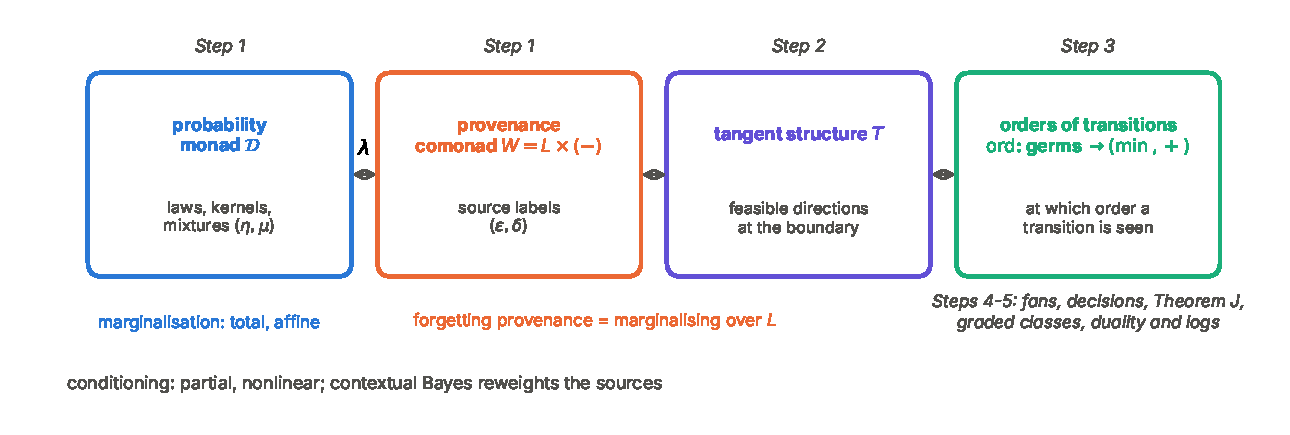
\includegraphics[width=\linewidth]{fig_architecture.pdf}
\caption{The layers and the step that builds each. Step 1 covers the probability monad, the provenance comonad and their
distributive law $\lambda$, with marginalisation and conditioning. Step 2 brings in the tangent structure on simplices with boundary
(\cref{sec:tangent}), Step 3 the orders of transitions (\cref{sec:orders}), Step 4a--4b several parameters and the order fan (\cref{sec:fan,sec:iterated}), Step 4c parameters as an object with decisions
on the fan (\cref{sec:para}), and Step 4d the probability-decorated fan and Theorem J on a statistical fan (\cref{sec:stat}). Step 4e collects the graded classes of maps
(\cref{sec:graded}), Step 4f resolves degenerate directions (\cref{sec:degen}), and Step 5 adds functions, duality and logs (\cref{sec:duality}).}\label{fig:architecture}
\end{figure}

\paragraph{What the layers are for.} The lab \cite{Lab} pools records from several sources, conditions on observed events, and asks how a
decision moves when the data move. Each operation is classical on its own. What the programme keeps needing is the \emph{compatibility} of
these operations. Does conditioning commute with pooling? What does forgetting a source label lose? How do these operations behave at the
boundary of the simplex, where the tangent companion \cite{TangentCompanion} lives? The layers of \cref{fig:architecture} answer these
questions one at a time. Each section has four parts: a definition, a compatibility statement, a proof, and checks with their limits. All
sets are finite.

\paragraph{A word on ``context''.} In the contextuality literature, and in our covers and lab papers, a \emph{context} is a measurement
context: a window of jointly observed variables \cite{AbramskyBrandenburger2011}. That is not the context of this paper. Here $L$ is a set of
\emph{provenances}, the sources records come from, and $W=L\times(-)$ is the \emph{provenance comonad} of the lab
\cite[Section ``sources'']{Lab}. The title keeps the broader word because later steps also carry measurement contexts.

\section{Related work and what is new}\label{sec:related}
\paragraph{Probability monads and Markov categories.} The finite distribution monad is the finite-support part of the Giry monad
\cite{Giry1982}. Its Kleisli category $\mathsf{FinStoch}$ is the basic Markov category \cite{Fritz2020}, in which joints, marginals and
independence are handled by the bimonoidal structure of probability monads \cite{FritzPerrone2018}. Effectuses give a related account of
normalisation and conditioning \cite{Jacobs2018}.

\paragraph{Conditioning, disintegration and inversion.} $\mathsf{FinStoch}$ has conditionals: every joint law factors through a kernel,
which is unique almost surely and arbitrary on null events \cite{Fritz2020}. Bayesian inversion reverses a kernel relative to a prior
\cite{ChoJacobs2019}. \Cref{sec:cond} uses a different, partial operation, event conditioning normalised by $p(A)$, because the geometry of the
later steps needs its behaviour as $p(A)\to0$. \Cref{prop:wall} shows exactly how the two differ at the wall.

\paragraph{Context, sheaves and descent.} Probability sheaves organise probability over a site of sample spaces \cite{Simpson2017}, and the
sheaf-theoretic account of contextuality organises it over measurement contexts \cite{AbramskyBrandenburger2011}. Our covers paper works
in that second setting. The provenance comonad is simpler: an explicit parameter carried alongside the law. Comonads of this product
form are the environment comonads of comonadic semantics \cite{UustaluVene2008}. Distributive laws between a monad and a comonad, and the
two-sided Kleisli category they produce, are classical \cite{BrookesVanStone1993,PowerWatanabe2002}.

\paragraph{Differential structure.} Tangent and differential categories axiomatise derivatives in general; the tangent companion builds a
weakened tangent structure on simplices with boundary, with graded classes of admissible maps \cite{TangentCompanion}. Step 2
(\cref{sec:tangent,sec:tw,sec:tm,sec:tc,sec:tp,sec:dbayes}) connects that work to the layers here.

\paragraph{What is new.} The distributive law of \cref{sec:comonad} is the strength of a commutative monad, and its two-sided Kleisli
category is the standard category of parameter-indexed kernels. We state and check them only to fix notation and types. The contribution of
Step 1 is a set of exact statements about failure of commutation that the later steps use:
\begin{itemize}
\item conditioning a pooled law reweights the sources (\cref{thm:bayes});
\item forgetting provenance loses source contrasts that every pooled table misses (\cref{prop:forget});
\item conditioning commutes with marginalisation only for cylinder events (\cref{prop:cond}(4));
\item event conditioning has no continuous extension to its wall (\cref{prop:wall}).
\end{itemize}
The research gap is their compatibility with a provenance comonad, with higher-order feasible differentiation on finite simplices, and
with decision functionals. In particular: how source reweighting, pooling and decisions interact with the boundary geometry and with the
graded classes.

\section{The finite distribution monad}\label{sec:monad}
\begin{definition}\label{def:monad}
For a finite set $X$, $\D X$ is the set of probability vectors on $X$. For $f:X\to Y$, $\D f$ is the push-forward. The unit is
$\eta_X(x)=\delta_x$. The multiplication $\mu_X:\D\D X\to\D X$ flattens a finitely supported distribution of distributions:
$\mu_X(\Phi)(x)=\sum_p\Phi(p)\,p(x)$.
\end{definition}
In the lab, pooling labelled batches is $\mu$. The Kleisli category is $\mathsf{FinStoch}$, the Markov category of
\cite[Section ``Markov categories'']{Lab}.

\section{The provenance comonad and the distributive law}\label{sec:comonad}
\begin{definition}[provenance]\label{def:context}
For a finite set $L$ of sources, $WX=L\times X$, with counit $\epsilon_X(l,x)=x$ (forget the source) and comultiplication
$\delta^W_X(l,x)=(l,(l,x))$ (copy it). The distributive law is
\[
\lambda_X:W\D X\longrightarrow\D WX,\qquad\lambda_X(l,p)=\delta_l\otimes p ,
\]
the law of $(l,x)$ with $l$ fixed and $x\sim p$.
\end{definition}

A comonad $W$ distributes over a monad $T$ through a transformation $WT\Rightarrow TW$ satisfying four axioms
\cite{PowerWatanabe2002}. The direction matters: $\lambda$ has the comonad outside on its source and the monad outside on its target.

\begin{proposition}[the four axioms]\label{prop:dist}
$\lambda$ is a distributive law of the comonad $W$ over the monad $\D$. Explicitly, the following commute for every finite $X$.
\begin{enumerate}
\item[(1)] \emph{Unit.} $\lambda_X\circ W\eta_X=\eta_{WX}:\ WX\to\D WX$.
\item[(2)] \emph{Multiplication.} $\lambda_X\circ W\mu_X=\mu_{WX}\circ\D\lambda_X\circ\lambda_{\D X}:\ W\D\D X\to\D WX$.
\item[(3)] \emph{Counit.} $\D\epsilon_X\circ\lambda_X=\epsilon_{\D X}:\ W\D X\to\D X$.
\item[(4)] \emph{Comultiplication.} $\D\delta^W_X\circ\lambda_X=\lambda_{WX}\circ W\lambda_X\circ\delta^W_{\D X}:\ W\D X\to\D WWX$.
\end{enumerate}
\[
\begin{tikzcd}[column sep=large]
W\D\D X \arrow[r,"\lambda_{\D X}"] \arrow[d,"W\mu_X"'] & \D W\D X \arrow[r,"\D\lambda_X"] & \D\D WX \arrow[d,"\mu_{WX}"] \\
W\D X \arrow[rr,"\lambda_X"'] & & \D WX
\end{tikzcd}
\qquad
\begin{tikzcd}[column sep=large]
W\D X \arrow[r,"\delta^W_{\D X}"] \arrow[d,"\lambda_X"'] & WW\D X \arrow[r,"W\lambda_X"] & W\D WX \arrow[d,"\lambda_{WX}"] \\
\D WX \arrow[rr,"\D\delta^W_X"'] & & \D WWX
\end{tikzcd}
\]
\end{proposition}

\begin{proof}
Evaluate both sides on an element.
\begin{itemize}
\item (1) $(l,x)\mapsto\lambda(l,\delta_x)=\delta_l\otimes\delta_x=\delta_{(l,x)}$.
\item (2) For $(l,\Phi)$ the left side is $\delta_l\otimes\mu\Phi$. On the right, $\lambda_{\D X}(l,\Phi)$ is the law of $(l,p)$ with
  $p\sim\Phi$; $\D\lambda$ sends it to the law of $\delta_l\otimes p$; $\mu$ flattens it to $\sum_p\Phi(p)\,\delta_l\otimes p=\delta_l\otimes\mu\Phi$.
\item (3) Pushing $\delta_l\otimes p$ forward along $(l,x)\mapsto x$ gives $p=\epsilon_{\D X}(l,p)$.
\item (4) The left side is the law of $(l,(l,x))$ with $x\sim p$. On the right, $(l,p)\mapsto(l,(l,p))\mapsto(l,\delta_l\otimes p)\mapsto
  \delta_l\otimes(\delta_l\otimes p)$, which is the same law.
\end{itemize}
Checks DL1--DL4 confirm each identity exactly, in rational arithmetic.
\end{proof}

\begin{proposition}[source-indexed Markov kernels]\label{prop:bikleisli}
The two-sided Kleisli category of $\lambda$ \cite{BrookesVanStone1993,PowerWatanabe2002} has the finite sets as objects. A morphism $X\to Y$
is a map $f:L\times X\to\D Y$, a Markov kernel indexed by the source. Composition is $g\circ f=\mu\circ\D g\circ\lambda\circ Wf\circ\delta^W$, which is
\[
(g\circ f)(l,x)(z)=\sum_yf(l,x)(y)\,g(l,y)(z) ,
\]
and the identity is $\eta\circ\epsilon$. One source is held throughout a composite.
\end{proposition}

\begin{proof}
$\delta^W$ copies $l$; $Wf$ uses one copy to produce $f(l,x)$; $\lambda$ pairs the other copy with it; $\D g$ applies $g(l,\cdot)$; $\mu$ sums.
Associativity and the identity laws follow from \cref{prop:dist}; DL5 checks them directly.
\end{proof}

\emph{Limits.} Sources here are known and discrete. A source drawn at random is a law on $L\times X$, an element of $\D WX$, and is
handled through $\lambda$ and $\mu$; a source that is uncertain inside a kernel is not.

\section{Marginalisation: total and affine}\label{sec:marg}
\begin{definition}\label{def:marg}
For $X=\prod_{i\in V}X_i$ and $S\subseteq V$, the marginalisation $M_S=\D\pi_S:\D X\to\D X_S$ is the push-forward along the projection.
\end{definition}

\begin{proposition}[marginalisation]\label{prop:marg}
\begin{enumerate}
\item[(1)] $M_S$ is total, and it preserves positivity and normalisation.
\item[(2)] $M_S\circ M_T=M_S$ for $S\subseteq T$, because $\pi_S\circ\pi_T=\pi_S$ and $\D$ is a functor.
\item[(3)] $M_S$ is affine (linear on measures), so $D^2M_S=0$.
\item[(4)] It commutes with forgetting provenance: $M_S\circ\D\epsilon=\D\epsilon\circ\D(W\pi_S)$ on $\D WX$.
\end{enumerate}
\end{proposition}

\begin{proof}
(1)--(3) are immediate from the push-forward. (4) $\pi_S\circ\epsilon=\epsilon\circ W\pi_S$ as maps $L\times X\to X_S$, and $\D$ is a functor
(DL6, DL11).
\end{proof}

\section{Conditioning: partial and nonlinear}\label{sec:cond}
\begin{definition}\label{def:cond}
For an event $A\subseteq X$, the conditioning operator is the partial map
\[
C_A:\D X\rightharpoonup\D X,\qquad C_A(p)=\frac{p\,\mathbf 1_A}{p(A)},\qquad\operatorname{Dom}C_A=\{p:p(A)>0\}.
\]
For $Y:X\to Z$ and $z\in Z$, write $C_z=C_{\{Y=z\}}$.
\end{definition}

\begin{proposition}[conditioning]\label{prop:cond}
\begin{enumerate}
\item[(1)] \emph{Partiality.} $C_A$ is defined exactly on $\{p(A)>0\}$, a relatively open subset of the simplex whose boundary is the
  face $\{p(A)=0\}$, the \emph{wall}.
\item[(2)] \emph{Total probability.} $p=\sum_{z:\,p(Y=z)>0}p(Y{=}z)\,C_z(p)$.
\item[(3)] \emph{Iteration.} $C_B(C_A(p))=C_{A\cap B}(p)$ whenever $p(A\cap B)>0$.
\item[(4)] \emph{With marginalisation.} If $A=\pi_S^{-1}(A')$ is a cylinder over the kept coordinates, then $M_S\circ C_A=C_{A'}\circ M_S$.
  For other events the square does not commute in general.
\item[(5)] \emph{Derivatives.} Write $N_A$ for multiplication by $\mathbf 1_A$ and $a(h)=h(A)$. Then
  \[
  DC_A(p)[h]=\frac{N_Ah}{a(p)}-\frac{N_Ap\,a(h)}{a(p)^2},\qquad
  D^2C_A(p)[h,k]=-\frac{N_Ah\,a(k)+N_Ak\,a(h)}{a(p)^2}+\frac{2N_Ap\,a(h)a(k)}{a(p)^3}.
  \]
  So conditioning is nonlinear, and $\|DC_A\|$ grows like $1/p(A)$ as $p$ approaches the wall.
\end{enumerate}
\end{proposition}

\begin{proof}
(1) The denominator. (2) $\sum_zp(Y{=}z)\,p\mathbf 1_{\{Y=z\}}/p(Y{=}z)=p$. (3) $(p\mathbf 1_A/p(A))\mathbf 1_B/(p(A\cap B)/p(A))=p\mathbf 1_{A\cap B}/p(A\cap B)$.
(4) With $A=\pi_S^{-1}(A')$, $M_S(p\mathbf 1_A)=(M_Sp)\mathbf 1_{A'}$ and $p(A)=M_Sp(A')$. (5) Differentiate the quotient (DL7, DL8, DL11).
\end{proof}

\begin{example}[the square fails for a non-cylinder event]\label{ex:square}
Take two binary variables, $R$ (recovered) and $H$ (high risk), and the law $p$ with $p(R{=}1,H{=}1)=\tfrac9{40}$,
$p(R{=}1,H{=}0)=\tfrac7{20}$, $p(R{=}0,H{=}1)=\tfrac14$ and $p(R{=}0,H{=}0)=\tfrac7{40}$ (the pooled law of \cref{ex:sources}).
Conditioning on $A=\{H=1\}$ and then keeping $R$ gives $P(R{=}1)=\tfrac9{19}$. The event projects to all of $R$, so conditioning the
marginal on its projection changes nothing: $P(R{=}1)=\tfrac{23}{40}$. The event reweights $R$ through the coordinate that was dropped
(DL13).
\end{example}

\begin{proposition}[conditioning at the wall]\label{prop:wall}
Let $A$ have at least two points, and let $p_0$ satisfy $p_0(A)=0$.
\begin{enumerate}
\item[(1)] $C_A$ has no continuous extension to $p_0$. Along the ray $p_t=(1-t)p_0+t\,q$, with $q$ supported in $A$, $C_A(p_t)=q$ for every
  $t>0$. So every law on $A$ is a limit at $p_0$.
\item[(2)] A conditional in the sense of $\mathsf{FinStoch}$ \cite{Fritz2020} exists at $p_0$: any kernel works on the null event $A$,
  and every choice gives the same joint law. The partial map $C_A$ and the categorical conditional therefore agree off the wall and part
  company exactly on it. There the conditional is defined by fiat, and no choice of it is continuous.
\end{enumerate}
\end{proposition}

\begin{proof}
(1) $p_t\mathbf 1_A=t\,q$ and $p_t(A)=t$. (2) Conditionals in $\mathsf{FinStoch}$ are unique only almost surely; on a null event they are
unconstrained. DL12 checks (1) exactly on three rays.
\end{proof}

\begin{figure}[!htbp]\centering
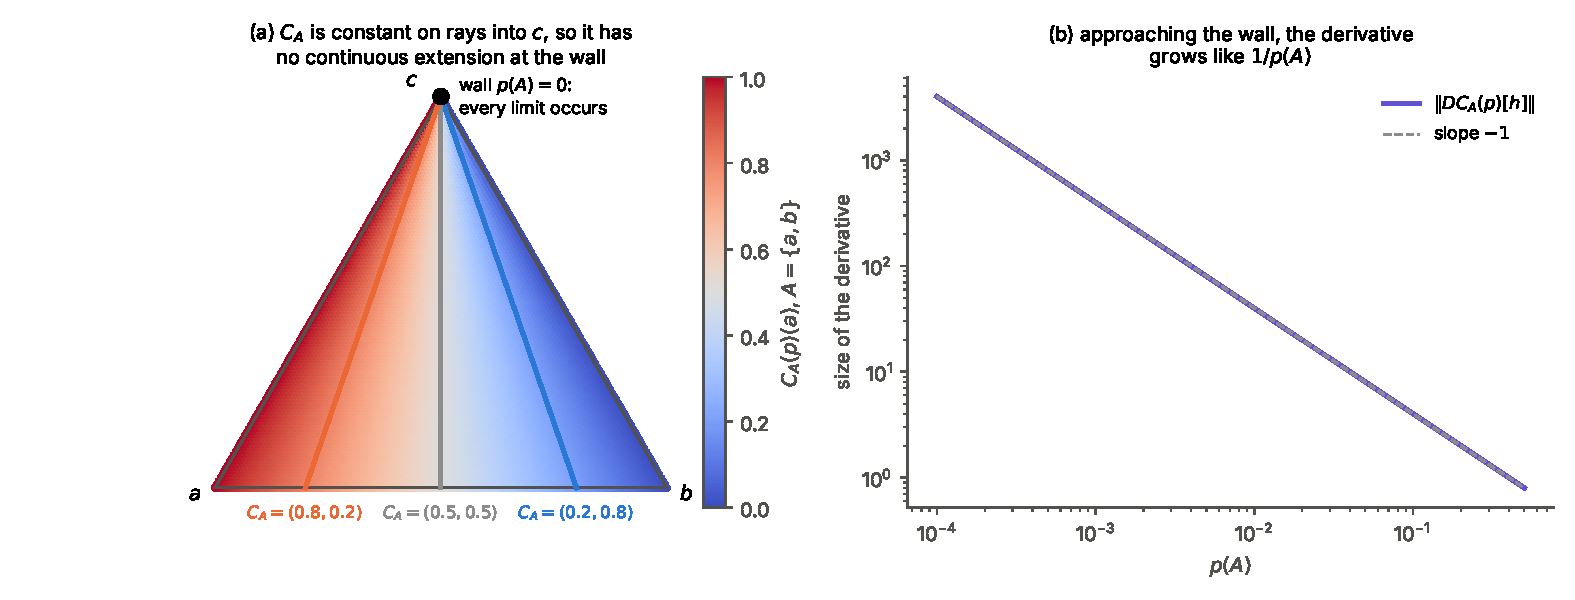
\includegraphics[width=\linewidth]{fig_wall.pdf}
\caption{Conditioning near the wall. (a) On the triangle of laws on $\{a,b,c\}$ with $A=\{a,b\}$, the colour is $C_A(p)(a)$. It is
constant along every ray into the vertex $c$, where $p(A)=0$, so every value is a limit there (\cref{prop:wall}). (b) The size of the
derivative of $C_A$ along a fixed direction, on log scales: slope $-1$, so it grows like $1/p(A)$ (\cref{prop:cond}(5)).}\label{fig:wall}
\end{figure}

This is why the later steps use the partial map. Its domain has a boundary, and the boundary carries the geometry. The categorical
conditional hides the wall by assigning arbitrary values there. The tangent companion already places $C_A$ in its second-order class of
maps \cite[Corollary ``the second-order subcategory'']{TangentCompanion}; Steps 2 and 3 take up corners and higher orders.

\section{Provenance with marginalisation and conditioning}\label{sec:context}
A pooled law is $\sum_l\pi_lp_l=\D\epsilon\bigl(\sum_l\pi_l\,\lambda(l,p_l)\bigr)$: label each source's law, mix, and forget the label.

\begin{theorem}[contextual Bayes decomposition]\label{thm:bayes}
Let $p_l\in\D X$ and weights $\pi_l$, and let $A$ be an event with $\sum_j\pi_jp_j(A)>0$. Then
\[
C_A\Bigl(\sum_l\pi_lp_l\Bigr)=\sum_{l:\,p_l(A)>0}\pi^A_l\,C_A(p_l),\qquad\pi^A_l=\frac{\pi_lp_l(A)}{\sum_j\pi_jp_j(A)} .
\]
Equivalently, conditioning the labelled law $\sum_l\pi_l\,\lambda(l,p_l)$ on $L\times A$ gives $\sum_l\pi^A_l\,\lambda(l,C_A(p_l))$. A known source
stays known ($C_{L\times A}(\delta_l\otimes p)=\delta_l\otimes C_A(p)$), and the source weights are updated by Bayes' rule. Conditioning within each
source and pooling with the \emph{old} weights gives the same law when $p_l(A)$ is the same for every source, and a different law in general.
\end{theorem}

\begin{proof}
$C_A(\sum_l\pi_lp_l)=\sum_l\pi_lp_l\mathbf 1_A/\sum_j\pi_jp_j(A)$, and $\pi_lp_l\mathbf 1_A=\pi_lp_l(A)\,C_A(p_l)$. The labelled form is the same
computation on $L\times X$. If all $p_l(A)$ are equal then $\pi^A=\pi$. If the $C_A(p_l)$ are affinely independent, the two pools agree only if
$\pi^A=\pi$ (DL9: exact; the old weights were wrong in all $40$ random cases).
\end{proof}

\begin{example}[two sources]\label{ex:sources}
Records come from small trials (source $1$, weight $\tfrac14$) and from a registry (source $2$, weight $\tfrac34$). Each records $R$
(recovered) and $H$ (high risk):
\begin{center}\small
\begin{tabular}{lcccc}\toprule
 & $R{=}1,H{=}1$ & $R{=}1,H{=}0$ & $R{=}0,H{=}1$ & $R{=}0,H{=}0$\\\midrule
source $1$ & $3/10$ & $1/2$ & $1/10$ & $1/10$\\
source $2$ & $1/5$ & $3/10$ & $3/10$ & $1/5$\\
pooled & $9/40$ & $7/20$ & $1/4$ & $7/40$\\\bottomrule
\end{tabular}
\end{center}
Condition on recovery, $A=\{R=1\}$. Recovery is likelier in source $1$ ($\tfrac45$ against $\tfrac12$), so the recovered records come
from it more often than its share: $\pi^A=(\tfrac{8}{23},\tfrac{15}{23})$. Among the recovered, the high-risk share is $\tfrac38$ in source $1$
and $\tfrac25$ in source $2$. Pooled with the Bayes weights, it is $\tfrac8{23}\cdot\tfrac38+\tfrac{15}{23}\cdot\tfrac25=\tfrac9{23}$, which is $C_A$ of
the pooled law. Pooled with the old weights it would be $\tfrac14\cdot\tfrac38+\tfrac34\cdot\tfrac25=\tfrac{63}{160}$, which is wrong
(\cref{fig:bayes}; DL13).
\end{example}

\begin{figure}[!htbp]\centering
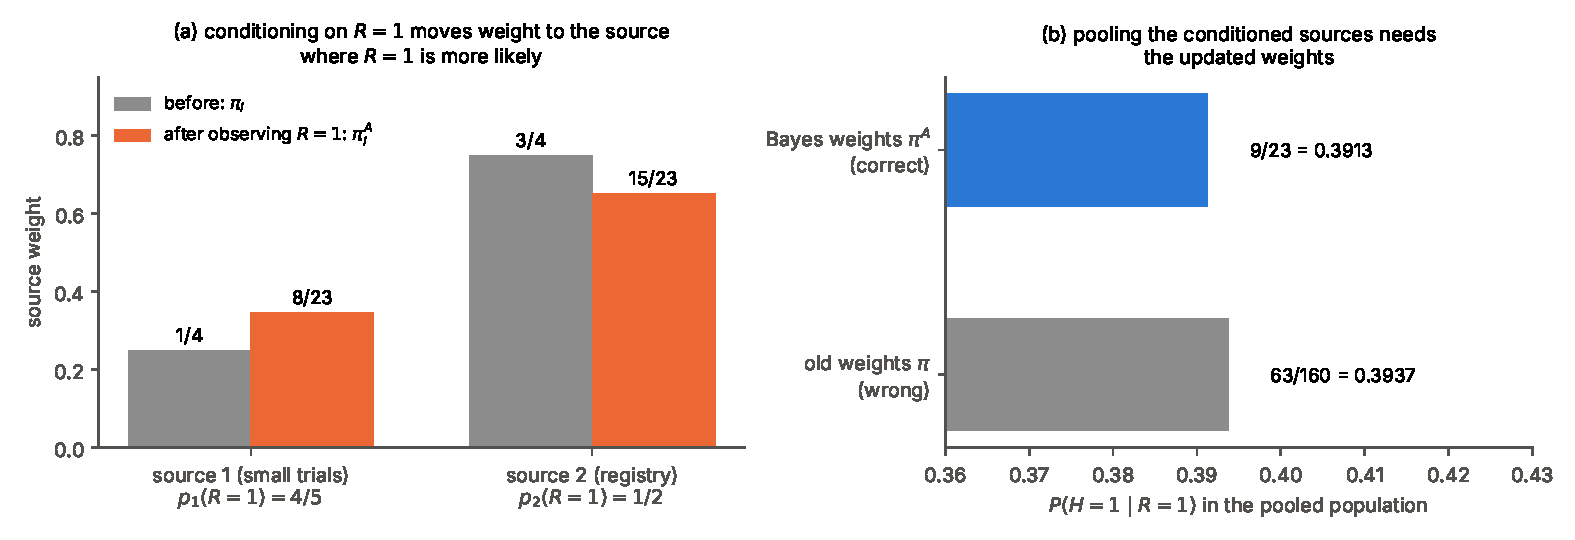
\includegraphics[width=\linewidth]{fig_bayes.pdf}
\caption{\Cref{ex:sources}. (a) Conditioning on $R=1$ moves weight towards the source in which recovery is likelier. (b) The high-risk
share among the recovered, pooled with the updated weights ($\tfrac9{23}$, correct) and with the old ones ($\tfrac{63}{160}$, wrong).}\label{fig:bayes}
\end{figure}

\begin{proposition}[forgetting provenance]\label{prop:forget}
Let $\Lambda=\sum_l\pi_l\,\lambda(l,p_l)\in\D WX$ be a labelled family, and $\D\epsilon(\Lambda)=\sum_l\pi_lp_l$ its pooled law.
\begin{enumerate}
\item[(1)] Forgetting is marginalisation over $L$. It commutes with every window marginalisation: the pooled window tables are the
  window tables of the pooled law.
\item[(2)] Forgetting is not injective. For any law $P$ and any direction $Q$ with $\sum Q=0$ and $P\pm Q\ge0$, the families
  $\tfrac12\lambda(l_1,P)+\tfrac12\lambda(l_2,P)$ and $\tfrac12\lambda(l_1,P+Q)+\tfrac12\lambda(l_2,P-Q)$ have the same pooled law and the
  same pooled window tables. Their labelled window tables differ on every window $S$ with $M_SQ\ne0$, by the source contrast $\pm M_SQ$.
\item[(3)] Forgetting does not commute with conditioning source by source: by \cref{thm:bayes}, conditioning reweights the sources.
\end{enumerate}
\end{proposition}

\begin{proof}
(1) is \cref{prop:marg}(4). (2) The pooled law is $P$ in both cases, and the labelled tables are $M_S(P\pm Q)$ for the two labels. (3) is
\cref{thm:bayes} (DL10).
\end{proof}

\begin{figure}[!htbp]\centering
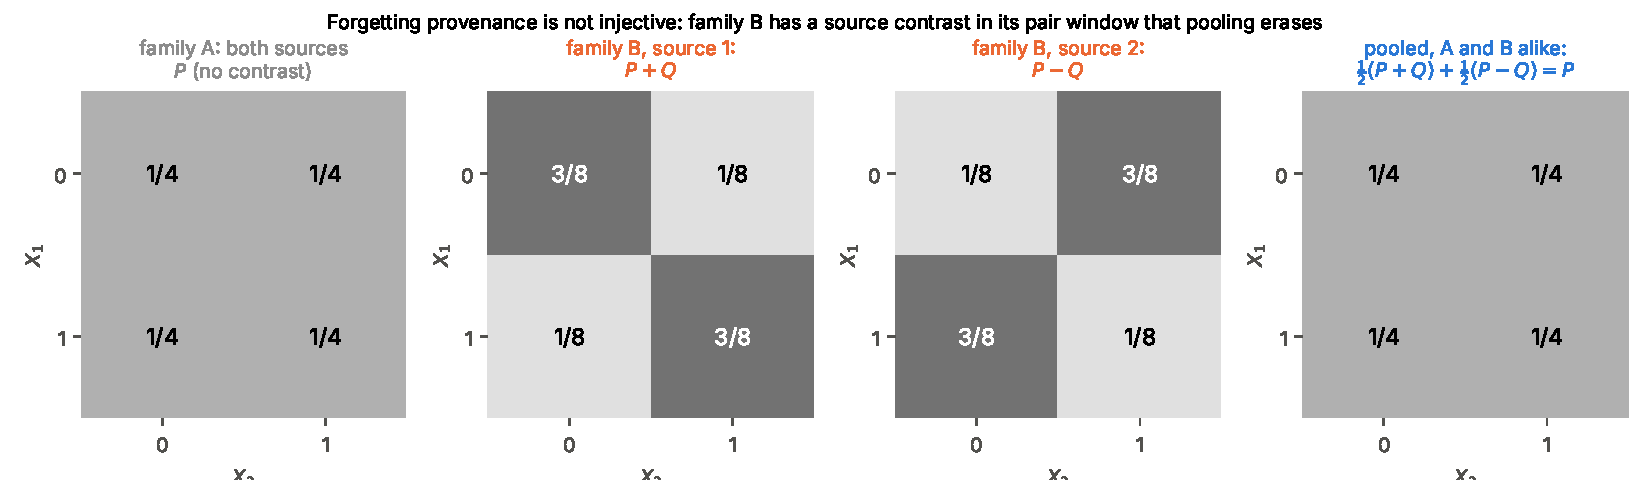
\includegraphics[width=\linewidth]{fig_forget.pdf}
\caption{\Cref{prop:forget}(2) on two binary variables: $P$ uniform and $Q=\tfrac18$ times the agreement contrast. Family A has no source
contrast; family B has opposite contrasts in its two sources. Both pool to $P$, so no pooled table can tell them apart; the labelled tables can.}\label{fig:forget}
\end{figure}

So a labelled cover sees source contrasts that pooling erases (\cref{fig:forget}). In the lab these contrasts are the degree-zero
discrepancy $\delta^0m_T$ of the labelled descent tower and the source statistic of Theorem J \cite[Theorem ``sources and bands'']{Lab}.
\Cref{prop:forget} says only that forgetting loses them. How large a contrast pooling can hide, in standard errors, is Theorem J's band, a
statistical statement derived in Step 4d (\cref{thm:Jfan}).

\section{Step 2: the tangent layer}\label{sec:tangent}
Step 2 brings the cone tangent structure of the tangent companion \cite{TangentCompanion} into the layers and asks how each Step 1
operation acts on feasible directions. Feasible directions matter because they are the ways data can move. In the lab, an adversary who
adds a share $\varepsilon$ of whole records from a law $Q$ moves the law $p$ to $(1-\varepsilon)p+\varepsilon Q$, that is, along $Q-p$
\cite[Part II]{Lab}. Every such direction is feasible, and every feasible direction is a positive multiple of one of them.

\paragraph{What we use from the tangent companion.} For a law $p$ on a finite set, the \emph{feasible cone} is
\[
C_p=\Bigl\{u:\ \textstyle\sum_xu(x)=0,\ u(x)\ge0\text{ wherever }p(x)=0\Bigr\},
\]
the directions $u$ for which $p+su$ is still a law for small $s\ge0$. It is a vector space exactly when $p$ has full support; at the
boundary it is only a cone, because mass can be added to an empty cell but not removed from it. $T\Delta=\{(p,u):u\in C_p\}$, and a map
$f$ acts by $Tf(p,u)=(f(p),Df(p)u)$. Higher orders are written in the Weil algebra $W_k=\R[e_1,\dots,e_k]/(e_1^2,\dots,e_k^2)$: a point of
$T^2\Delta$ is $p+u\,e_1+v\,e_2+w\,e_1e_2$, and $T^2f$ is $f$ evaluated on such points. Membership is decided cell by cell by the
lexicographic lemma \cite[Lemma ``the lexicographic lemma'']{TangentCompanion}. A map is a \emph{morphism at order $k$} if $T^kf$ maps
$T^k$ of its domain into $T^k$ of its codomain. Stochastic matrices are morphisms at every order. A smooth map is a morphism at order $2$
iff it passes the \emph{second-order corner criterion}: at each output cell $y$ with $f_y(p)=0$, the Hessian of $f_y$ is non-negative on
pairs from $K_y=C_p\cap\ker Df_y(p)$ \cite[Theorem ``second-order cone morphisms'']{TangentCompanion}. The criterion is not automatic:
$q\mapsto\bigl(1-(q_1-q_2)^2,(q_1-q_2)^2,0\bigr)$ keeps first-order feasibility and fails at second order.

Pooling has several simplices as inputs (the weights and each source), so we need the criterion on a product.

\begin{lemma}[the criterion on products of simplices]\label{lem:products}
Let $Y=\Delta_{n_1}\times\dots\times\Delta_{n_r}$ and let $f:Y\to\Delta_m$ be smooth. Then $T^kY=\prod_jT^k\Delta_{n_j}$, and $T^2f$ maps the fibre
of $T^2Y$ over $x$ into $T^2\Delta_m$ iff, for every output cell $y$ with $f_y(x)=0$, $D^2f_y(x)\ge0$ on $K_y\times K_y$, where $K_y=C_x\cap\ker
Df_y(x)$ and $C_x=\prod_jC_{x_j}$.
\end{lemma}

\begin{proof}
$T$ preserves finite products and the lexicographic lemma holds row by row for any polyhedron \cite[Lemma ``the lexicographic
lemma'']{TangentCompanion}. The proof of \cite[Theorem ``second-order cone morphisms'']{TangentCompanion} then runs block by block: $Df_y\ge0$
on $C_x$, so in each block the gradient is constant on the support and no smaller on the empty cells, and the remaining steps are
unchanged.
\end{proof}

Our implementation of \cref{lem:products} rejects the counterexample above (TL5, negative control), so the passes reported below are not
vacuous.

\section{Tangent and provenance}\label{sec:tw}
\begin{proposition}[$T$ commutes with $W$]\label{prop:tw}
Let $L$ be finite and discrete.
\begin{enumerate}
\item[(1)] $T^k(L\times\Delta_X)=L\times T^k\Delta_X$: a source label has no tangent directions.
\item[(2)] $T^k\lambda:(l,c)\mapsto\delta_l\otimes c$, applied coefficient by coefficient, maps $L\times T^k\Delta_X$ into $T^k\Delta_{L\times X}$, and
  the unit, counit and comultiplication axioms of \cref{prop:dist} hold after applying $T^k$, for every $k$.
\item[(3)] Forgetting provenance, $\D\epsilon$, is a stochastic matrix, so it is a morphism at every order. At first order it maps $C_q$
  onto $C_{\D\epsilon(q)}$, with the lift of \cref{prop:tm}(2) below.
\end{enumerate}
\end{proposition}

\begin{proof}
(1) $L$ is a finite disjoint union of points. (2) Each map in the three axioms is affine in the law, and $T^k$ of an affine map is that map
applied to every coefficient. The image is in $T^k\Delta_{L\times X}$ because the cells off row $l$ have all coefficients $0$, and the cells of
row $l$ carry the coefficients of $c$. (3) $\D\epsilon$ is marginalisation over $L$ (\cref{prop:forget}(1)); apply \cref{prop:tm}. TL1
and TL3 check this.
\end{proof}

The multiplication axiom (2) of \cref{prop:dist} involves $\D\D X$, which is not a polyhedron, so the cone structure does not apply to it
directly. Its restriction to $n$ fixed sources is the pooling map of \cref{sec:tp}.

\begin{proposition}[the source face]\label{prop:face}
Let $q=\lambda(l,p)=\delta_l\otimes p$. The map $\lambda(l,\cdot)$ embeds $\Delta_X$ as the face of $\Delta_{L\times X}$ of laws supported on
$\{l\}\times X$.
\begin{enumerate}
\item[(1)] $D\lambda_l:C_p\to C_q$ is injective. Its image is the set of $u\in C_q$ that vanish off row $l$: the directions along the face.
\item[(2)] Every $u\in C_q$ decomposes uniquely as
  \[
  u=D\lambda_l(v)+m\,(Q'-q),\qquad v\in C_p,\quad m\ge0,\quad Q'\in\Delta_{(L\setminus\{l\})\times X}\ (\text{if }m>0),
  \]
  where $m$ is the mass $u$ puts off row $l$. A feasible direction leaves the face exactly when it injects whole records under other labels.
\item[(3)] After forgetting provenance, injection and drift are the same. The injection of records from $Q$ under a new label $l'$, the
  direction $\delta_{l'}\otimes Q-q$, and the drift of source $l$ towards $Q$, the direction $\delta_l\otimes(Q-p)$, both map to $Q-p$
  under $D\epsilon$. The relabelling direction $\delta_{l'}\otimes p-q$ is feasible and maps to $0$.
\end{enumerate}
\end{proposition}

\begin{proof}
(1) $\lambda(l,\cdot)$ is affine and injective; its derivative puts $v$ on row $l$. (2) $q$ vanishes off row $l$, so $u\ge0$ there. Let $m$ be
the sum of those entries and $Q'$ their normalisation. Set $v=u_l+m\,p$, with $u_l$ the row-$l$ part of $u$. Then $\sum v=\sum u_l+m=0$, and $v\ge0$
wherever $p=0$, because $u_l\ge0$ there. The off-row part of $u$ fixes $m$ and $Q'$, and then $v$, so the decomposition is unique.
(3) $D\epsilon$ sums over labels: $\delta_{l'}\otimes Q-\delta_l\otimes p\mapsto Q-p$, $\delta_l\otimes(Q-p)\mapsto Q-p$, and
$\delta_{l'}\otimes p-\delta_l\otimes p\mapsto0$. TL2 checks (1)--(2) on $200$ directions and TL3 checks (3).
\end{proof}

\begin{figure}[!htbp]\centering
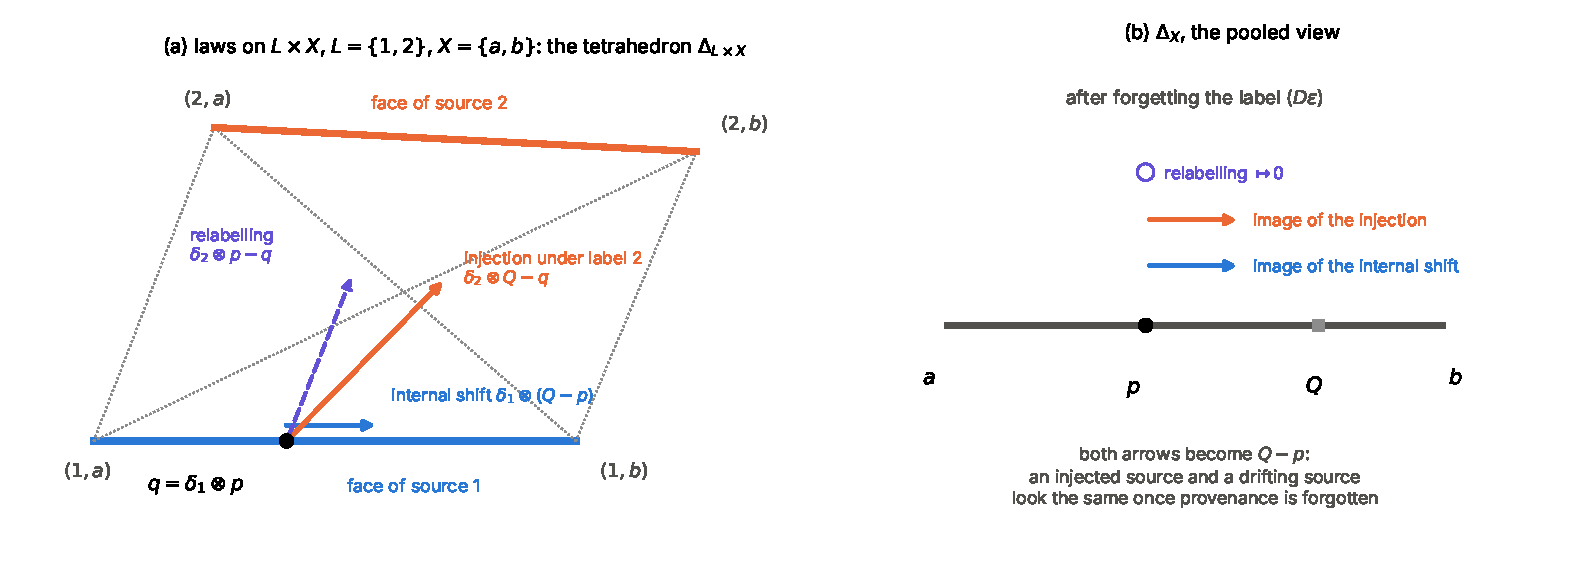
\includegraphics[width=\linewidth]{fig_face.pdf}
\caption{\Cref{prop:face} with two sources and two outcomes. (a) The labelled laws form a tetrahedron; each source's laws form an edge (a
face). At $q=\delta_1\otimes p$ the internal shift stays on the face of source $1$, while injection under label $2$ and relabelling leave it.
(b) After forgetting the label, the injection and the internal shift have the same image $Q-p$, and relabelling disappears.}\label{fig:face}
\end{figure}

So the provenance comonad separates two things that the pooled tangent space identifies: a source that drifts and a source that is
added (\cref{fig:face}). This is the infinitesimal form of \cref{prop:forget}(2). A screen on the pooled law alone can detect that data
moved along $Q-p$, but not whether an existing source changed or a new one was injected. Only labelled tables tell these apart.

\section{Tangent and marginalisation}\label{sec:tm}
\begin{proposition}[marginalisation on feasible directions]\label{prop:tm}
Let $S$ be a set of coordinates and $M_S$ the marginalisation.
\begin{enumerate}
\item[(1)] $M_S$ is a stochastic matrix, so $T^kM_S=M_S$ coefficient by coefficient maps $T^k\Delta_X$ into $T^k\Delta_{X_S}$ for every $k$,
  and $D^2M_S=0$.
\item[(2)] At first order it is \emph{onto}: every $v\in C_{M_Sp}$ is $M_Su$ for
  \[
  u(x)=v(x_S)\,p(x\mid x_S)\ \text{ if }M_Sp(x_S)>0,\qquad u(x)=v(x_S)/|\pi_S^{-1}(x_S)|\ \text{ otherwise},
  \]
  and this $u$ lies in $C_p$.
\item[(3)] Its kernel on directions, $\{u:\sum u=0,\ M_Su=0\}$, has dimension $|X|-|X_S|$. These are the directions the window $X_S$
  cannot see; for a cover they are the common kernel of all its windows, the hidden channels of \cite[Theorem F]{Lab}.
\end{enumerate}
\end{proposition}

\begin{proof}
(1) \cite[Proposition ``morphisms'']{TangentCompanion}. (2) $M_Su(x_S)=v(x_S)\sum_{x\mapsto x_S}p(x\mid x_S)=v(x_S)$ in the first case, and the
same in the second. Feasibility: if $p(x)=0$ and $M_Sp(x_S)>0$ then $u(x)=0$; if $M_Sp(x_S)=0$ then $v(x_S)\ge0$, so $u(x)\ge0$. (3) $M_S$ is onto
the zero-sum directions on $X_S$, so the kernel dimension is $(|X|-1)-(|X_S|-1)$. TL4 checks all three on $200$ laws with zeros.
\end{proof}

\begin{example}[a direction the window cannot see]\label{ex:invisible}
In \cref{ex:sources}, order the cells $(R,H)=(1,1),(1,0),(0,1),(0,0)$ and take $u=(1,-1,0,0)$: move records from ``recovered, low risk'' to
``recovered, high risk''. The $R$ window sees nothing: $M_{\{R\}}u=0$. But the answer of \cref{ex:sources} moves fast. By
\cref{prop:cond}(5), with $p(R{=}1)=\tfrac{23}{40}$, the derivative of $P(H{=}1\mid R{=}1)$ along $u$ is $u(1,1)/p(R{=}1)=\tfrac{40}{23}$. A
window that misses a coordinate misses exactly the directions to which a conditional on that coordinate responds.
\end{example}

\section{Tangent and conditioning}\label{sec:tc}
\begin{proposition}[conditioning on feasible directions]\label{prop:tc}
Let $p(A)>0$.
\begin{enumerate}
\item[(1)] $DC_A(p)$ maps $C_p$ \emph{onto} $C_{C_Ap}$. A lift of $v\in C_{C_Ap}$ is $u=p(A)\,v$ (zero off $A$).
\item[(2)] The kernel of $DC_A(p)$ on directions is $\{u:\sum u=0,\ N_Au=u(A)\,C_Ap\}$, of dimension $|X|-|A|$. These directions change
  how much mass $A$ carries, or move mass outside $A$, without changing its shape inside $A$.
\item[(3)] $C_A$ passes the second-order corner criterion at every point of its domain, corners included
  \cite[Corollary ``the second-order subcategory'']{TangentCompanion}.
\item[(4)] Near the wall the lift shrinks: the move of $p$ needed for a given move $v$ of $C_Ap$ has size $p(A)\,|v|$, so
  $\|DC_A(p)\|\sim1/p(A)$. At the wall itself $C_A$ is undefined and has no continuous extension (\cref{prop:wall}).
\end{enumerate}
\end{proposition}

\begin{proof}
(1) With $DC_A(p)u=(N_Au-u(A)C_Ap)/p(A)$ (\cref{prop:cond}(5)): if $p(x)=0$ with $x\in A$, then $C_Ap(x)=0$ and $u(x)\ge0$, so the image is $\ge0$
there. The image sums to $0$. For the lift, $u=p(A)v$ has $u(A)=0$, so $DC_A(p)u=v$; it is feasible because the zeros of $C_Ap$ in $A$ are zeros
of $p$. (2) Read off from the formula; the condition fixes $N_Au$ up to the scalar $u(A)$, leaving $1+(|X|-|A|)$ free coordinates minus the
sum constraint. (4) From (1) and \cref{prop:cond}(5). TL5 checks (1), (2) and (4), and re-checks (3) with \cref{lem:products} at three
corners and with $900$ sampled points of $T^2\Delta$.
\end{proof}

In the worked example, moving the high-risk share among the recovered by $0.01$ takes a move of only $0.01\cdot\tfrac{23}{40}\approx0.006$
in the joint law, made inside $R=1$. Were recovery rare, say $p(R{=}1)=0.01$, the same move would take $0.0001$. Conditioning on a rare
event amplifies small injections, and \cref{prop:tc}(4) is the exact rate.

\section{Tangent and pooling}\label{sec:tp}
Pooling $n$ sources is the restriction of the monad multiplication to $n$ fixed sources:
\[
\mu_n:\Delta_n\times(\Delta_X)^n\to\Delta_X,\qquad\mu_n(w,p_1,\dots,p_n)=\sum_iw_ip_i=\D\epsilon\Bigl(\sum_iw_i\,\lambda(i,p_i)\Bigr).
\]
It is bilinear, not affine, so the fact that stochastic matrices are morphisms does not cover it. The next theorem does, at every order.
Write $H=[0,\infty)$ for the half-line.

\begin{theorem}[$T^kH$ is generated by elementary tensors]\label{thm:tensor}
For every $k$, $T^kH\subset W_k$ is the convex cone generated by the products $u_1(e_1)\,u_2(e_2)\cdots u_k(e_k)$ with each
$u_i=x_i+y_ie_i\in TH$ (that is, $x_i>0$, or $x_i=0\le y_i$). Consequently $T^kH$ is closed under the product of $W_k$.
\end{theorem}

\begin{proof}
Write $G_k$ for the cone generated by the elementary tensors. Induction on $k$; $G_0=T^0H=H$.

$G_k\subseteq T^kH$: a point of $T^kH=T(T^{k-1}H)$ is $\alpha+\beta e_k$ with $\alpha+s\beta\in T^{k-1}H$ for all small $s\ge0$. For $g\in G_{k-1}$ and
$u_k=x+ye_k$: if $x>0$ then $g\,x+s\,g\,y=(x+sy)g\in T^{k-1}H$ for small $s$; if $x=0\le y$ then $0+s\,yg\in T^{k-1}H$. $T^kH$ is a convex cone.

$T^kH\subseteq G_k$: let $\alpha+\beta e_k\in T^kH$ and fix $s>0$ with $\alpha+s\beta\in T^{k-1}H$. Then
\[
\alpha+\beta e_k=\alpha\,\bigl(1-\tfrac1se_k\bigr)+\bigl(\beta+\tfrac1s\alpha\bigr)\,e_k .
\]
Here $\alpha\in T^{k-1}H$, and $\beta+\tfrac1s\alpha=\tfrac1s(\alpha+s\beta)\in T^{k-1}H$ because it is a cone; both lie in $G_{k-1}$ by induction.
$1-\tfrac1se_k$ and $e_k$ lie in $TH$. So the right side is in $G_k$.

Products: $W_k=W_1^{\otimes k}$ as algebras, so the product of two elementary tensors is $\prod_i(u_iv_i)(e_i)$, and
$TH$ is closed under products: $(x+ye)(x'+y'e)=xx'+(xy'+x'y)e$, which lies in $TH$ when both factors do. By bilinearity the cone $G_k$ is
closed under products.
\end{proof}

\begin{corollary}[pooling is a morphism at every order]\label{cor:pool}
\begin{enumerate}
\item[(1)] The product of laws $(x,y)\mapsto x\otimes y$ and the labelled joint $J(w,p_1,\dots,p_n)=\sum_iw_i\,\lambda(i,p_i)$ map $T^k$ of their
  domains into $T^k$ of their codomains, for every $k$.
\item[(2)] So does pooling, $\mu_n=\D\epsilon\circ J$. Its derivative maps the product of feasible cones into $C_{\mu_n}$, including at
  sources of weight $0$ and cells where every source vanishes. $D^3\mu_n=0$.
\end{enumerate}
\end{corollary}

\begin{proof}
(1) Each cell of $x\otimes y$ is a product $x_iy_j$, and each cell $(i,x)$ of $J$ is $w_ip_i(x)$. By \cref{thm:tensor} every cell of the image
is in $T^kH$. The equations hold because $\sum_xp_i(x)=1$ and $\sum_iw_i=1$ hold in $W_k$. (2) $\D\epsilon$ is stochastic; $\mu_n$ is bilinear,
so its third derivative vanishes.
\end{proof}

\Cref{cor:pool}(1) also proves the statement of \cite[Proposition ``morphisms'']{TangentCompanion} about products of laws, which was
checked there but not proved. TL9 checks \cref{thm:tensor} directly: an explicit decomposition into elementary tensors for $1510$
points of $T^kH$, $k\le4$, and closure under products for all pairs of a grid when $k=2$ and $100{,}000$ sampled pairs when $k=3$.
TL6 checks the second-order criterion for $\mu_n$ at corners (\cref{lem:products}), including a source of weight $0$. At the
level of individual cells the reason is simple. If $w_i>0$ at a cell where the pool vanishes, then $p_i$ vanishes there and the first-order
term $w_iu_i$ keeps it non-negative. If $w_i=0$, the term $a_ip_i$ does. If both vanish, every entry is non-negative.

\begin{remark}[where the pooling paradox lives]
The tangent companion shows that two data sets choosing the same act can pool to one choosing the other, through the curvature of the
decision boundary \cite[Proposition ``pooling paradox = curvature'']{TangentCompanion}. \Cref{cor:pool} locates the paradox: pooling
itself is as tame as a Markov kernel at every order. Of the maps met so far, only conditioning (partial, with a pole) and the decision
functional bend.
\end{remark}

\section{Differentiating the contextual Bayes decomposition}\label{sec:dbayes}
\Cref{thm:bayes} expresses $C_A\circ\mu_n$ through the Bayes weights. Differentiating it splits every sensitivity of a pooled conditional
into two terms.

\begin{proposition}[reweighting and within-source terms]\label{prop:dbayes}
Let $\sum_j\pi_jp_j(A)>0$, and move the weights along $a$ and the sources along $u_1,\dots,u_n$. Then
\begin{gather*}
D(C_A\circ\mu_n)[a,u]=\underbrace{\sum_l\dot\pi^A_l\,C_A(p_l)}_{\text{reweighting}}+\underbrace{\sum_l\pi^A_l\,DC_A(p_l)[u_l]}_{\text{within sources}},\\
\dot\pi^A_l=\frac{a_lp_l(A)+\pi_lu_l(A)}{Z}-\pi^A_l\,\frac{\sum_j\bigl(a_jp_j(A)+\pi_ju_j(A)\bigr)}{Z},
\end{gather*}
with $Z=\sum_j\pi_jp_j(A)$ (sources with $p_l(A)=0$ drop out of the second sum). If only the weights move, only the reweighting term remains;
if only the sources move and $p_l(A)$ is the same for all $l$ and stays so, only the within-source term remains.
\end{proposition}

\begin{proof}
Differentiate $C_A(\sum\pi_lp_l)=\sum_l\pi^A_lC_A(p_l)$ (\cref{thm:bayes}) by the product rule; $\dot\pi^A$ is the derivative of
$\pi_lp_l(A)/Z$. TL7 checks the identity on $100$ random configurations.
\end{proof}

\begin{example}[how fast the answer moves with the small-trial share]\label{ex:sens}
In \cref{ex:sources}, let the small-trial share $\pi_1$ vary, with $\pi_2=1-\pi_1$. The answer is
\begin{gather*}
f(\pi_1)=P(H{=}1\mid R{=}1)=\frac{\tfrac15+\tfrac1{10}\pi_1}{\tfrac12+\tfrac3{10}\pi_1},\\
f(\tfrac14)=\tfrac9{23},\qquad f'(\tfrac14)=-\tfrac{16}{529}\approx-0.030,\qquad f''(\tfrac14)=\tfrac{384}{12167}\approx0.032 .
\end{gather*}
Only the weights move, so \cref{prop:dbayes} gives $f'=\dot\pi^A_1\,(\tfrac38-\tfrac25)$ with $\dot\pi^A_1=\tfrac{640}{529}\approx1.21$: the
Bayes weight moves $1.21$ times as fast as the prior weight, and the answer moves by that times the gap between the sources' answers.
Raising the small-trial share from $25\%$ to $26\%$ lowers the answer by about $0.0003$, and the second-order term adds about
$0.0000016$. Since $f$ is a ratio of affine functions, the answer stays between the two sources' answers, $\tfrac38$ and $\tfrac25$, for
every share (\cref{fig:sens}; TL8, exact).
\end{example}

\begin{figure}[!htbp]\centering
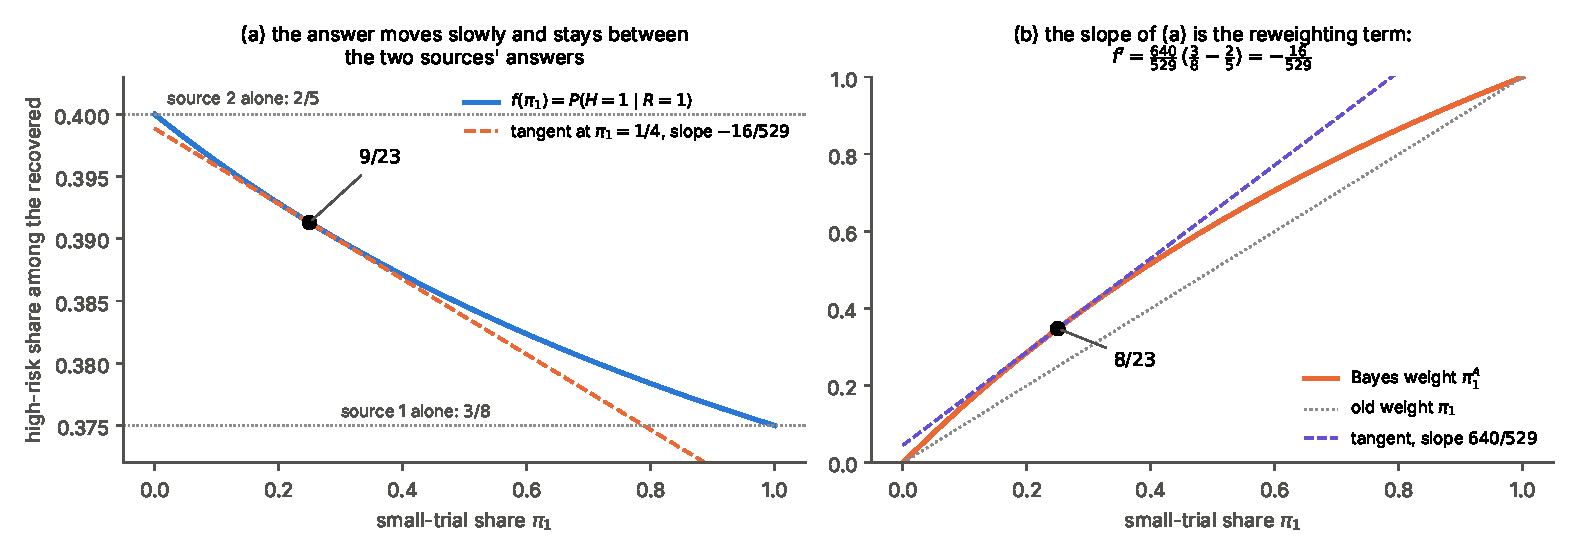
\includegraphics[width=\linewidth]{fig_sens.pdf}
\caption{\Cref{ex:sens}. (a) The answer $P(H{=}1\mid R{=}1)$ as the small-trial share varies, with its tangent at $\tfrac14$. (b) The
Bayes weight of the small trials, against the old weight. The slope of (a) is the slope of (b) times the gap $\tfrac38-\tfrac25$ between
the sources' answers.}\label{fig:sens}
\end{figure}

\section{Strata and jumps}\label{sec:jumps}
Derivatives describe gradual change. Conditioned probabilities can also change suddenly, and a source can drop out of the explanation of
an event. This section says exactly when this happens, for finite sets. It has three results.
\begin{itemize}
\item The sources that survive conditioning are explicit, and they cut the space of labelled laws into strata (\cref{thm:support}).
\item Inside the domain of conditioning nothing jumps. The rate of change is at most $2/P(A)$, so a sudden change needs the event to
  become rare (\cref{thm:regimes}(1)--(2)).
\item At the wall $P(A)=0$ the limit depends on the leading jet of the path, not on the point reached. A smooth (analytic) passage
  through the wall is removable; a jump needs a kink at the wall, a non-analytic path, or a jump of the law itself (\cref{thm:regimes}(3)--(5)).
\end{itemize}
The last point is where points give way to functions. At the wall, the conditioned state is a function of how the path arrives, its germ,
and not of where it arrives.

\paragraph{The state and the operator.} A source-labelled state $\Theta=(\pi_l,p_l)_{l\in L}$ is the labelled law
$\Lambda=\sum_l\pi_l\,\lambda(l,p_l)\in\Delta_{L\times X}$, with pooled law $P=\D\epsilon(\Lambda)$. Conditioning the state is
\[
\mathfrak C_A=C_{L\times A}:\Delta_{L\times X}\rightharpoonup\Delta_{L\times X}.
\]
By \cref{thm:bayes}, the $L$-marginal of $\mathfrak C_A(\Lambda)$ is the vector of Bayes weights $\pi^A$, and its row $l$, normalised, is $C_A(p_l)$.

\begin{theorem}[provenance support]\label{thm:support}
Let $P(A)=\sum_l\pi_lp_l(A)>0$.
\begin{enumerate}
\item[(1)] The surviving sources are $\operatorname{supp}\pi^A=L_A(\Lambda)=\{l:\pi_lp_l(A)>0\}$. A source drops out if it has weight $0$, or
  if it gives $A$ probability $0$.
\item[(2)] $\pi^A_l=\pi_lp_l(A)/P(A)$, and for surviving $l,j$ the posterior odds are the prior odds times the likelihood ratio:
  $\pi^A_l/\pi^A_j=(\pi_l/\pi_j)\,(p_l(A)/p_j(A))$.
\item[(3)] Forgetting commutes with conditioning: $\D\epsilon\circ\mathfrak C_A=C_A\circ\D\epsilon$, so $\sum_l\pi^A_lC_A(p_l)=C_A(P)$.
\item[(4)] A source with $\pi_l>0$ and $p_l(A)=0$ has no row in $\mathfrak C_A(\Lambda)$. Its own conditional $C_A(p_l)$ is undefined, and nothing
  requires it.
\end{enumerate}
So the domain of $\mathfrak C_A$ is the union of the strata $\mathcal S_J(A)=\{\Lambda:L_A(\Lambda)=J\}$ for non-empty $J\subseteq L$. On each stratum
$\mathfrak C_A$ is a rational map with a positive denominator, and the wall is $\mathcal S_\varnothing(A)$.
\end{theorem}

\begin{proof}
$\mathfrak C_A(\Lambda)(l,x)=\pi_lp_l(x)\mathbf 1_A(x)/P(A)$. Summing over $x$ gives (1) and (2), and the odds follow. Summing over $l$ gives (3).
Row $l$ vanishes iff $\pi_lp_l(A)=0$, which is (4). SJ1 checks all four exactly on $291$ random families with zero weights and
zero likelihoods.
\end{proof}

\begin{proposition}[four questions]\label{prop:four}
Let $P(A)>0$ and $n=|L|$.
\begin{enumerate}
\item[(1)] \emph{When are the weights preserved?} $\pi^A=\pi$ iff $p_l(A)=P(A)$ for every $l$ with $\pi_l>0$.
\item[(2)] \emph{When do conditioning and pooling commute?} Suppose every source of positive weight has $p_l(A)>0$. Pooling the
  conditioned sources with the old weights gives $C_A(P)$ iff $\sum_l(\pi^A_l-\pi_l)\,C_A(p_l)=0$. This follows from (1). It is equivalent to (1)
  when the $C_A(p_l)$ are affinely independent. It holds whatever the weights do when the $C_A(p_l)$ coincide.
\item[(3)] \emph{What happens to the fibres of forgetting?} $\mathfrak C_A$ maps the fibre $\D\epsilon^{-1}(P)$ onto the fibre $\D\epsilon^{-1}(C_AP)$: a
  labelled law $\Lambda'$ over $C_AP$ comes from $\Lambda=P(A)\Lambda'+\delta_{l_0}\otimes P|_{X\setminus A}$. The dimensions split as
  \[
  \underbrace{(n-1)\,|\operatorname{supp}P|}_{\text{fibre over }P}=\underbrace{(n-1)\,|\operatorname{supp}P\cap A|}_{\text{fibre over }C_AP}+
  \underbrace{(n-1)\,|\operatorname{supp}P\setminus A|}_{\text{lost by conditioning}} .
  \]
  Conditioning keeps the provenance ambiguity on $A$ and discards the provenance off $A$. It never resolves ambiguity.
\item[(4)] \emph{Can provenance be recovered after conditioning?} Not from the pooled law: every $w\in\Delta_L$ is the posterior
  provenance of some state in the fibre over $P$ (lift $\sum_lw_l\,\lambda(l,C_AP)$ by (3)). With known source laws and unknown weights,
  $\pi^A$ is determined by $C_A(P)$ iff the $C_A(p_l)$ with $p_l(A)>0$ are linearly independent. If they are, so are those $p_l$:
  conditioning can destroy identifiability but cannot create it.
\end{enumerate}
\end{proposition}

\begin{proof}
(1) By \cref{thm:support}(2), $\pi^A_l=\pi_l$ iff $p_l(A)=P(A)$ or $\pi_l=0$. (2) The old pool minus $C_A(P)$ is $\sum_l(\pi_l-\pi^A_l)C_A(p_l)$ by
\cref{thm:support}(3). The weight differences sum to $0$, so this is an affine relation among the $C_A(p_l)$. (3) $\D\epsilon(\Lambda)=P(A)\,C_AP+P|_{X\setminus A}=P$,
and on $L\times A$ the law $\Lambda$ is $P(A)\Lambda'$, so $\mathfrak C_A(\Lambda)=\Lambda'$. A fibre of forgetting over $Q$ is a product, over $x\in\operatorname{supp}Q$,
of simplices of dimension $n-1$ (how $Q(x)$ is split among the sources). The preimages of a fixed $\Lambda'$ are free exactly in the cells off
$A$. (4) The first claim is (3). Mixture weights are determined by the mixture iff the components are linearly independent, which for
laws is the same as affinely independent, because a linear relation among laws has coefficients summing to $0$. If $\sum_lc_lp_l=0$, then
restricting to $A$ gives $\sum_lc_l\,p_l(A)\,C_A(p_l)=0$, so independence of the $C_A(p_l)$ forces every $c_lp_l(A)=0$, hence $c_l=0$. SJ2 and SJ3
check all four, (3) with explicit lifts and with ranks of sampled fibres.
\end{proof}

For example, take $p_1=(\tfrac14,\tfrac14,\tfrac12,0)$ and $p_2=(\tfrac38,\tfrac38,0,\tfrac14)$ on $\{a,b,c,d\}$ with $A=\{a,b\}$, and equal
weights. Conditioning moves the weights to $(\tfrac25,\tfrac35)$, yet pooling with the old weights is still correct, because both sources
condition to the same law. The two sources are distinguishable before conditioning and indistinguishable after it.

\begin{theorem}[regimes of conditioned probability]\label{thm:regimes}
Let $t\mapsto\Lambda_t$ be a path in $\Delta_{L\times X}$ and write $P_t(A)=\Lambda_t(L\times A)$.
\begin{enumerate}
\item[(1)] \emph{Regular regime.} $\|D\mathfrak C_A(\Lambda)h\|_1\le2\|h\|_1/\Lambda(L\times A)$. So if $\Lambda_t$ is continuous (or $C^k$) and $P_t(A)\ge\varepsilon>0$,
  then $\mathfrak C_A(\Lambda_t)$, $\pi^A(t)$ and $C_A(P_t)$ are continuous (or $C^k$), and
  \[
  \|\pi^A(t_1)-\pi^A(t_0)\|_1\le2\int_{t_0}^{t_1}\frac{\|\dot\Lambda_t\|_1}{P_t(A)}\,dt .
  \]
  A complete change of the source that explains $A$ ($\|\Delta\pi^A\|_1=2$) needs $\int\|\dot\Lambda_t\|_1/P_t(A)\,dt\ge1$. At speed at most $v$, with
  $P_t(A)\ge\varepsilon$, that takes time at least $\varepsilon/v$.
\item[(2)] \emph{Changes of stratum.} If $P_t(A)$ stays positive while a source leaves or joins $L_A$, then $\pi^A_l(t)$ tends to $0$ or
  leaves it continuously. The leaving source's own conditional $C_A(p_l(t))$ may have no limit, because that source is at its own wall,
  but it carries vanishing weight. The conditioned state can be continuous while a source's own conditional jumps.
\item[(3)] \emph{The wall, one side.} Let $\Lambda_{t^*+s}=\sum_jc_js^j$ for small $s\ge0$ (a polynomial or convergent series), with $P_{t^*}(A)=0$ and
  $P_t(A)\not\equiv0$. Let $m$ be the least $j$ with $c_j|_{L\times A}\ne0$. Then $c_m|_{L\times A}\ge0$, and
  \[
  \lim_{s\downarrow0}\mathfrak C_A(\Lambda_{t^*+s})=C_{L\times A}(c_m),
  \]
  with error $O(s)$. The limiting provenance is the Bayes weighting of the leading jet. The sources that survive are those whose
  mass on $A$ vanishes at the least order $m$; the others become extinct at the wall. Different jets give different limits, and every
  law on $L\times A$ occurs (\cref{prop:wall}).
\item[(4)] \emph{Analytic passages are removable.} If $\Lambda_t$ is analytic on both sides of $t^*$ and $P_t(A)\not\equiv0$, then $\mathfrak C_A(\Lambda_t)$ extends analytically
  through $t^*$, and its two one-sided limits agree.
\item[(5)] \emph{Where jumps come from.} So if $\mathfrak C_A(\Lambda_t)$ jumps at $t^*$, then one of the following holds:
  \begin{itemize}
  \item the law $\Lambda_t$ itself jumps;
  \item the path reaches the wall with a kink, and the conditionals of its two one-sided leading jets differ;
  \item the path is not analytic at the wall, and then the limit need not exist.
  \end{itemize}
\end{enumerate}
\end{theorem}

\begin{proof}
(1) On $L\times X$, $D\mathfrak C_A(\Lambda)h=(N_Ah-h(L\times A)\,\mathfrak C_A\Lambda)/\Lambda(L\times A)$ (\cref{prop:cond}(5)), and
$\|N_Ah\|_1+|h(L\times A)|\le2\|h\|_1$. Taking the $L$-marginal, a stochastic map, does not increase $\|\cdot\|_1$. Then integrate.
(2) $\pi^A_l=\Lambda_t(l,A)/P_t(A)$ is continuous, and so is the rest, by (1).
(3) Each cell of $L\times A$ is non-negative, so its first non-zero coefficient is positive. Below order $m$ every such coefficient is $0$, so
$\mathfrak C_A(\Lambda_{t^*+s})=(s^mc_m|_{L\times A}+O(s^{m+1}))/(s^mc_m(L\times A)+O(s^{m+1}))$.
(4) A non-negative analytic function vanishing at $t^*$ is $(t-t^*)^{m_c}h_c(t)$ with $m_c$ even and $h_c(t^*)>0$. Divide numerator and
denominator by $(t-t^*)^m$, $m=\min m_c$. The denominator becomes $\sum_{m_c=m}h_c(t^*)>0$ at $t^*$.
(5) combines (1)--(4).

SJ4 checks (1) on $100$ random paths (the largest ratio to the bound is $0.42$) and (2) on an oscillating extinction. SJ5 checks (3)
exactly on $200$ polynomial paths, (4) on a two-sided passage, and the kink of (5).
\end{proof}

\begin{example}[gradual, then sudden]\label{ex:jumps}
Two sources of weight $\tfrac12$ each. Source $1$ produces $a$ or $c$, source $2$ produces $b$ or $c$, and $A=\{a,b\}$ (``a flagged
record''). Over time, source $1$ stops producing flagged records and source $2$ starts:
\[
\Lambda_t(1,a)=\eta+\max(-t,0),\qquad\Lambda_t(2,b)=\eta+\max(t,0),\qquad t\in[-\tfrac14,\tfrac14],
\]
with the rest of each source's mass on $c$. The source weights never change, and $P_t(A)=2\eta+|t|$ changes gradually
(\cref{fig:jumps}(a)). But the source that explains a flagged record switches:
\[
\pi^A_1(t)=\frac{\eta+\max(-t,0)}{2\eta+|t|}
\]
falls from $\tfrac34$ to $\tfrac14$ over an interval of length exactly $4\eta$, with slope $-1/(4\eta)$ at $t=0$ (\cref{fig:jumps}(b)). The smaller the
gap $\eta$ between the path and the wall, the more sudden the switch, as \cref{thm:regimes}(1) requires. At $\eta=0$ the path touches the
wall with a kink: the one-sided jets are $\delta_{(1,a)}$ and $\delta_{(2,b)}$, and $\pi^A_1$ jumps from $1$ to $0$, a complete replacement of the
explaining source. A smooth path into the wall behaves differently. Along $p_t=(t,\ t(1-t),\ 1-t-t(1-t))$ on $\{a,b,c\}$, the event
$\{a,b\}$ becomes impossible at $t=0$. Yet $C_A(p_t)$ tends to $(\tfrac12,\tfrac12,0)$, the conditional of the leading jet $(1,1,0)$. Here
$C_A(p_t)=(\tfrac1{2-t},\tfrac{1-t}{2-t},0)$ moves at a bounded rate all the way in (SJ5, SJ6).
\end{example}

\begin{figure}[!htbp]\centering
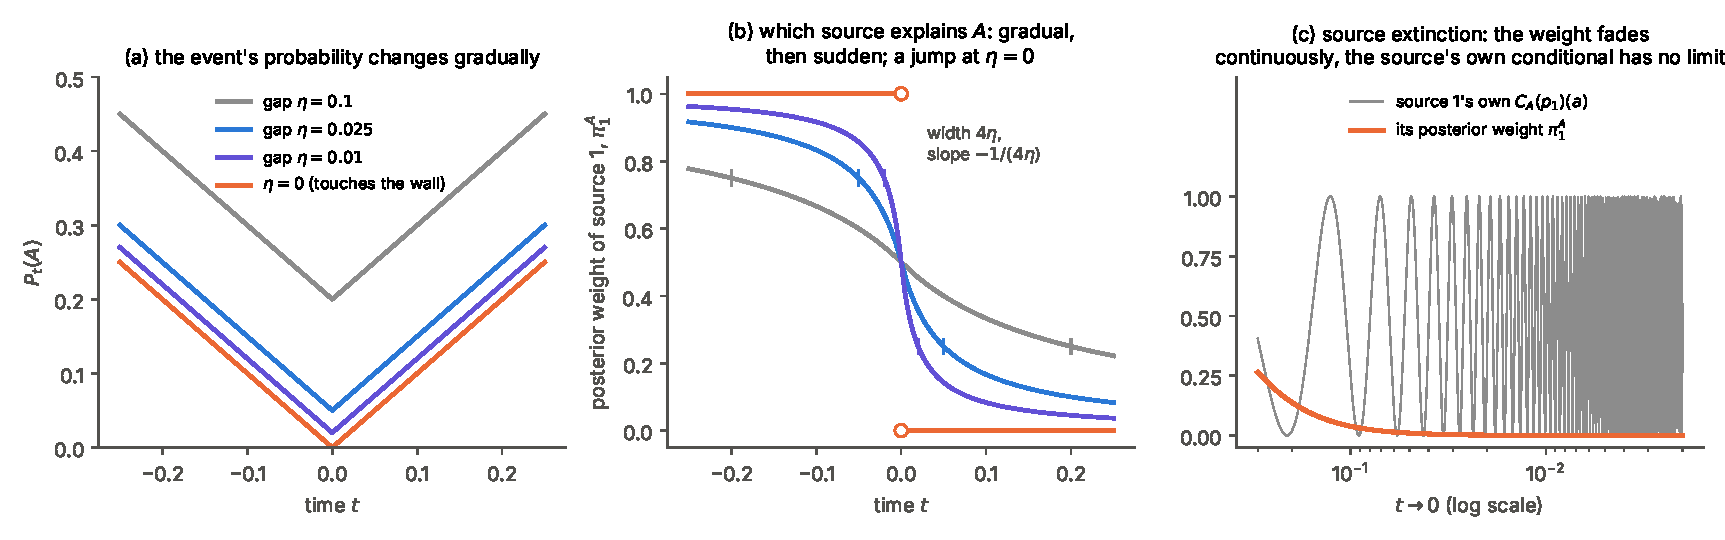
\includegraphics[width=\linewidth]{fig_jumps.pdf}
\caption{\Cref{ex:jumps} and \cref{thm:regimes}. (a) $P_t(A)$ changes gradually for every gap $\eta$. (b) The posterior weight of source $1$
switches over a window of width $4\eta$ (ticks at $\pm2\eta$), and jumps at $\eta=0$, where the path meets the wall with a kink. (c) Source
extinction inside the domain. Source $1$'s posterior weight fades continuously to $0$, while its own conditional oscillates without a limit (SJ4).}\label{fig:jumps}
\end{figure}

\begin{center}\small
\resizebox{\linewidth}{!}{\begin{tabular}{lllll}\toprule
regime & the law & $P(A)$ & the conditioned state & checks\\\midrule
regular & continuous & $\ge\varepsilon$ & continuous, rate $\le2/\varepsilon$ & SJ4\\
change of stratum & continuous & $\ge\varepsilon$ & continuous; a leaving source's own conditional may jump & SJ4\\
near the wall & continuous & small, $>0$ & continuous but steep: gradual, then sudden & SJ6\\
wall, analytic & analytic & $\to0$ & removable; limit = conditional of the leading jet & SJ5\\
wall, kink & one-sided analytic & $\to0$ & jumps iff the one-sided jets condition differently & SJ5, SJ6\\
outside jump & jumps & any & may jump & ---\\\bottomrule
\end{tabular}}
\end{center}

\begin{remark}[transition operators and what is not covered]
An outside jump replaces $\Lambda$ by $J(\Lambda)$ for a map $J$ of $\Delta_{L\times X}$. If $J$ is a stochastic matrix it preserves total probability
and positivity. It is \emph{provenance-consistent}, preserving every source weight $\pi_l$, when it acts row by row through a source-indexed
kernel: a morphism of the two-sided Kleisli category (\cref{prop:bikleisli}). Even then $\pi^A$ can jump, because the $p_l(A)$ can. The hybrid
dynamics of regular flows interrupted by such operators is not developed here. Neither is the analogue of \cref{thm:regimes} beyond
finite sets, where the answer depends on the notion of conditional probability and on the topology, and needs separate care.
\end{remark}

\section{Step 2 in one table}\label{sec:step2table}
\begin{center}\small
\resizebox{\linewidth}{!}{\begin{tabular}{lllll}\toprule
operation & domain & first order on cones & order $2$ & every order\\\midrule
$\D\epsilon$, $M_S$, $\lambda(l,\cdot)$ & total & onto (explicit lift) & yes & yes (stochastic)\\
$\mu_n$ (pooling) & total & into & yes & yes (\cref{cor:pool})\\
$C_A$ (conditioning) & $p(A)>0$ & onto, pole $1/p(A)$ & yes & yes (\cref{thm:graded}, Step 4e)\\
$\mathfrak C_A$ (labelled) & $P(A)>0$, strata $\mathcal S_J$ & continuous, rate $\le2/P(A)$ & yes & yes on the domain; at the wall: the leading jet (\cref{thm:regimes})\\\bottomrule
\end{tabular}}
\end{center}
Conditioning beyond order two was left open when Step 2 was written. The tangent companion gives only a necessary condition at order $k$
\cite[Proposition ``order $k$: necessity, and order three'']{TangentCompanion}. Step 4e settles it: conditioning is subtraction-free, so it keeps
feasibility at every order (\cref{thm:graded}).

\section{Step 3: the order of a transition}\label{sec:orders}
\Cref{thm:regimes}(3) shows that at the wall the conditioned state is decided by the leading term of the path, not by the point it reaches.
So a transition carries more structure than ``continuous or not''. Each source approaches the event at its own \emph{order}, and the orders
decide which sources survive, how fast the others disappear, whether the two sides of a transition agree, and how sudden a near-miss is.
This step makes that precise. The main tool is one observation: on non-negative quantities, ``order'' turns sums into minima and products
into sums. Positivity is what makes this exact.

\paragraph{Germs and orders.} We look at quantities near a time $t^*$ from one side and write $s=t-t^*\downarrow0$. A \emph{germ} is a
function of $s$ for small $s>0$, up to equality near $0$. To compare germs we need them to be comparable, and the natural setting is a
\emph{Hardy field} $\mathcal H$: a field of germs of differentiable functions closed under differentiation \cite{Hardy1910,Rosenlicht1983}. Every
element of a Hardy field has a limit in $[-\infty,\infty]$, so the ratio of two non-zero elements always has a limit. Examples are the
generalised power sums $\sum_ic_is^{a_i}$, Hardy's exp-log functions (such as $s^{3/2}$, $e^{-1/s}$, $1/\log\tfrac1s$), and the germs definable in an
o-minimal structure. Write $\mathcal H_+$ for the positive germs together with $0$. For $f,g\in\mathcal H_+\setminus\{0\}$ write $f\asymp g$ if $f/g$
tends to a finite non-zero limit. The \emph{order} $v(f)$ is the class of $f$, ordered by $v(f)<v(g)$ iff $g/f\to0$ (so $g$ vanishes faster);
set $v(0)=\infty$. For $f\sim c\,s^a$ with $c>0$, $v(f)$ is the exponent $a$ and $c$ is the \emph{leading coefficient}. Flat germs such as
$e^{-1/s}$ have orders beyond every power: $v(s^n)<v(e^{-1/s})$ for all $n$.

\begin{theorem}[orders tropicalise]\label{thm:tropical}
On $\mathcal H_+$,
\[
v(f+g)=\min\{v(f),v(g)\},\qquad v(fg)=v(f)+v(g).
\]
If $f\sim c\,s^a$ and $g\sim d\,s^b$, then $fg\sim cd\,s^{a+b}$, and $f+g\sim c\,s^a$ if $a<b$, $d\,s^b$ if $b<a$, and $(c+d)\,s^a$ if $a=b$. So
$v$ is a homomorphism from the semiring $(\mathcal H_+,+,\times)$ onto the tropical semiring $(\Gamma\cup\{\infty\},\min,+)$ of orders. Positivity is
necessary: $s+s^2$ and $-s$ have order $1$, and their sum has order $2$.
\end{theorem}

\begin{proof}
For positive $f,g$, $\max(f,g)\le f+g\le2\max(f,g)$, so $f+g\asymp\max(f,g)$, the germ of least order. On a tie the leading coefficients are both
positive and add without cancelling. Products are immediate. OR1 checks this exactly on $500$ pairs of non-negative power sums, and checks
the counterexample.
\end{proof}

\begin{corollary}[the order calculus of the layers]\label{cor:calculus}
Let a labelled path $\Lambda_s(l,x)=\pi_l(s)\,p_{l,s}(x)$ have all its cells in $\mathcal H_+$. Write
\[
m_l=v\bigl(\Lambda_s(l,A)\bigr)=v(\pi_l)+v\bigl(p_{l,s}(A)\bigr),\qquad m=v\bigl(P_s(A)\bigr)=\min_lm_l .
\]
\begin{center}\small
\begin{tabular}{lll}\toprule
operation & order & leading coefficient\\\midrule
labelling $\pi_lp_l(x)$ & $v(\pi_l)+v(p_l(x))$ & product\\
pooling $P(x)=\sum_l\Lambda(l,x)$ & $\min_lv(\Lambda(l,x))$ & sum over the sources of least order\\
marginalisation $M_SP(x_S)$ & minimum over the fibre & sum over the cells of least order\\
conditioning $\mathfrak C_A\Lambda(l,x)$ & $v(\Lambda(l,x))-m$ & divided by the leading coefficient of $P(A)$\\
Bayes weight $\pi^A_l$ & $m_l-m$ & $c_l/c$\\\bottomrule
\end{tabular}
\end{center}
Here $c_l$ and $c$ are the leading coefficients of $\Lambda_s(l,A)$ and $P_s(A)$.
\end{corollary}

\begin{proof}
Every operation is built from sums and products of non-negative germs, with one division by $P_s(A)$. Apply \cref{thm:tropical}. OR2 checks
every row exactly on $200$ random labelled paths.
\end{proof}

\begin{theorem}[the hierarchy of transitions]\label{thm:hierarchy}
Let the cells of $\Lambda_s$ on $L\times A$ lie in one Hardy field, not all zero. Then $\mathfrak C_A(\Lambda_s)$ has a limit as $s\downarrow0$. Its support
is the set of cells of least order $m$, and the surviving sources are $\{l:m_l=m\}$. When the cells are asymptotic to powers, the limit is
the normalised vector of leading coefficients of order $m$. In particular:
\begin{enumerate}
\item[(1)] \emph{Common order.} Several sources reach the event at the least order. All survive, with limiting weights $c_l/\sum_{j:m_j=m}c_j$.
\item[(2)] \emph{Unequal order.} A source with $m_l>m$ disappears from the explanation, at rate $\pi^A_l(s)\sim(c_l/c)\,s^{m_l-m}$. Its
  \emph{extinction order} is $m_l-m$. For generalised power sums, the conditioned state converges at rate $O(s^\delta)$, where $\delta$ is the gap
  from $m$ to the next exponent appearing on $L\times A$.
\item[(3)] \emph{One-sided mismatch.} The two sides of $t^*$ carry independent data $(m^\pm_l,c^\pm_l)$. The one-sided limits differ iff the two
  leading conditionals differ. If the path is analytic across $t^*$, every order on $L\times A$ is even and the two sides agree
  (\cref{thm:regimes}(4)). Infinite differentiability is not enough: with $\Lambda_t(1,a)=e^{-1/t^2}$ for $t<0$ and $\Lambda_t(2,b)=e^{-1/t^2}$ for $t>0$
  (zero otherwise), every derivative exists, and the explaining source jumps from $1$ to $2$.
\item[(4)] \emph{Flat approach.} Germs with every derivative zero at $s=0$ still have orders, beyond all powers, and inside a Hardy field the
  limit exists. For example, $e^{-1/s}/\log\tfrac1s$ against $e^{-1/s}$ has limiting share $0$, reached only logarithmically slowly. Outside a
  Hardy field the limit can fail to exist: $e^{-1/s}(1+\sin\tfrac1s)$ against $e^{-1/s}$ has a share that oscillates in $[0,\tfrac23]$.
\end{enumerate}
So whether a conditioned probability has a limit is a question of comparability, and what the limit is a question of order.
\end{theorem}

\begin{proof}
In a Hardy field each ratio $f_c/f_{c'}$ of positive cells has a limit in $[0,\infty]$. Choose a cell $c^*$ of least order. Then $f_c/f_{c^*}\to r_c<\infty$ for
every $c$, with $r_c>0$ iff $v(f_c)=m$. So $\mathfrak C_A(\Lambda_s)(c)=(f_c/f_{c^*})/\sum_{c'}(f_{c'}/f_{c^*})\to r_c/\sum r_{c'}$, and the denominator is at least $1$.
For powers, $r_c$ is the ratio of leading coefficients. (1) and (2) are \cref{cor:calculus}. The rate in (2) comes from expanding numerator
and denominator one exponent further. (3) The two sides are separate germs; the analytic case is \cref{thm:regimes}(4); the flat example
is $C^\infty$ because $e^{-1/t^2}$ is. (4) $e^{-1/s}$ and $\log\tfrac1s$ lie in Hardy's exp-log field. $1+\sin\tfrac1s$ is not eventually comparable
with $1$. Checks: OR3 for (1)--(2), exactly on $200$ paths plus a fractional example; OR4 for (3); OR5 for (4), computed in log space.
\end{proof}

\begin{proposition}[the order is the level of the tangent tower that sees the transition]\label{prop:tower}
Let $\Lambda_s=\sum_jc_js^j$ be analytic with $P_0(A)=0$, and let $j^k\Lambda=\sum_{j\le k}c_js^j$ be its $k$-jet.
\begin{enumerate}
\item[(1)] For $k<m$ the $k$-jet has no mass on $L\times A$, so it cannot be conditioned. For $k\ge m$ it has the same limit as the path.
\item[(2)] In the Weil-algebra picture of Step 2, the $k$-jet is the point $\Lambda(e_1+\dots+e_k)$ of $T^k\Delta_{L\times X}$. Its coefficient on $e^S$
  is $|S|!\,c_{|S|}$. On $L\times A$ the first non-zero coefficients sit at $|S|=m$, which are the coefficients the lexicographic lemma reads first.
\end{enumerate}
So a transition of order $m$ is invisible to $T^k$ for $k<m$ and determined at level $m$ of the tower.
\end{proposition}

\begin{proof}
(1) The coefficients of order $<m$ vanish on $L\times A$, and the limit depends only on $c_m$ (\cref{thm:hierarchy}). (2)
$(e_1+\dots+e_k)^j=j!\sum_{|S|=j}e^S$ because $e_i^2=0$. OR6 checks (1) on $200$ paths for $k\le5$, and (2) with the Weil-algebra arithmetic.
\end{proof}

\begin{example}[order and suddenness]\label{ex:order}
Repeat \cref{ex:jumps} at order $m$: $\Lambda_t(1,a)=\eta+\max(-t,0)^m$ and $\Lambda_t(2,b)=\eta+\max(t,0)^m$. Then
$\pi^A_1(t)=(\eta+\max(-t,0)^m)/(2\eta+|t|^m)$ runs from $\tfrac34$ to $\tfrac14$ over $[-(2\eta)^{1/m},(2\eta)^{1/m}]$ exactly. For the same gap
$\eta=\tfrac1{1000}$, the switch has width $0.004$ at order $1$, $0.089$ at order $2$, and $0.25$ at order $3$. A higher-order approach is more
gradual. For $m\ge2$ the curve is flat at the crossing, where both sources explain the event equally, and the change happens on either side
of it (\cref{fig:orders}(b); OR7, exact). At $\eta=0$ every order gives the same jump from $1$ to $0$: the order shapes the approach, not the
jump.
\end{example}

\begin{figure}[!htbp]\centering
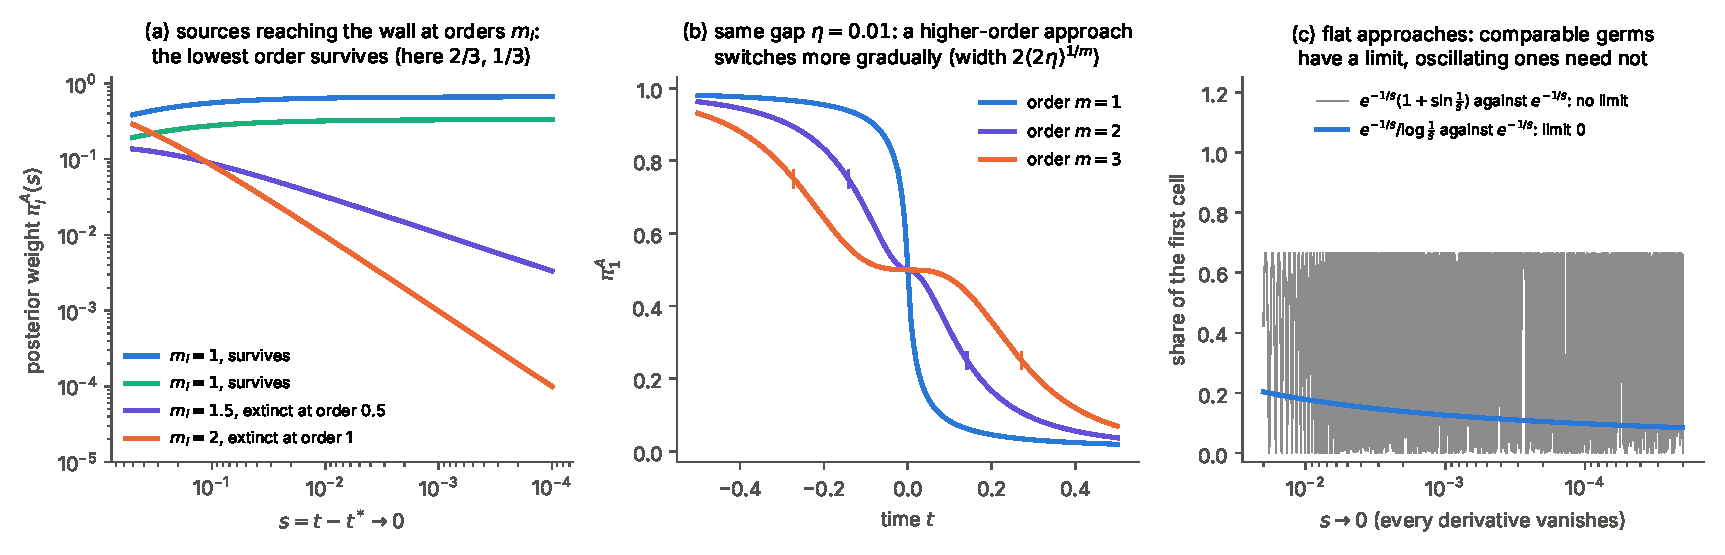
\includegraphics[width=\linewidth]{fig_orders.pdf}
\caption{Orders of transitions. (a) Four sources reach the wall at orders $1,1,\tfrac32,2$. The two of order $1$ survive with weights
$\tfrac23,\tfrac13$, and the others vanish at their extinction orders $\tfrac12$ and $1$, the slopes on log scales (\cref{thm:hierarchy}(1)--(2)).
(b) \Cref{ex:order}: the same gap, approached at orders $1,2,3$ (ticks at $\pm(2\eta)^{1/m}$). (c) Flat approaches: a comparable pair has a limit,
an oscillating pair has none (\cref{thm:hierarchy}(4)).}\label{fig:orders}
\end{figure}

\begin{center}\small
\resizebox{\linewidth}{!}{\begin{tabular}{lllll}\toprule
approach & orders on $L\times A$ & surviving sources & conditioned limit & checks\\\midrule
common order & several $m_l=m$ & all of least order & weights $c_l/\sum c_j$ & OR3\\
unequal order & some $m_l>m$ & least order only & others vanish like $s^{m_l-m}$ & OR3\\
one-sided mismatch & $(m^-,c^-)\ne(m^+,c^+)$ & may differ by side & jump iff the leading conditionals differ & OR4\\
analytic passage & even, equal on both sides & same on both sides & removable & SJ5, OR4\\
flat, Hardy & beyond all powers & least order & exists & OR5\\
flat, not Hardy & not comparable & undefined & may not exist & OR5\\\bottomrule
\end{tabular}}
\end{center}

\emph{Limits of Step 3.} Orders are taken along one-parameter paths; several parameters are Step 4a--4b (\cref{sec:fan}). Decisions taken on conditioned laws at the wall, whose acts depend on the leading
coefficients and, on ties, on the next order, are Step 4c (\cref{thm:decisionfan}). The graded classes of maps planned for Step 3 in the earlier draft move to Step 4, with the
contextual second-order theorem.

\section{Step 4a: several parameters at once}\label{sec:fan}
In the lab, several things move together: the share of a source, the rate at which it produces an event, the size of a batch. A
one-parameter path is a choice of how they move together, and the data do not make that choice. This section lets $d$ parameters
$\varepsilon=(\varepsilon_1,\dots,\varepsilon_d)$ tend to $0$ independently, in the open orthant. Its message, shown by five small examples, is that
the order of \cref{sec:orders} becomes a \emph{fan}: a finite division of the possible rates into cones, each with its own winning sources.

\paragraph{Setting.} Each cell of $\Lambda_\varepsilon$ on $L\times A$ is a polynomial $f_c(\varepsilon)=\sum_\alpha a_{c,\alpha}\varepsilon^\alpha$, non-negative on the orthant
near $0$, and $\Phi(\varepsilon)=\mathfrak C_A(\Lambda_\varepsilon)$ is the conditioned state. A \emph{monomial arc} is $\varepsilon_i=c_is^{w_i}$ with weights $w\in\mathbb Q^d_{>0}$
(how fast each parameter vanishes) and coefficients $c\in\R^d_{>0}$, and $s\downarrow0$. A \emph{Puiseux arc} has $\varepsilon_i=c_is^{w_i}(1+o(1))$.
The \emph{tropical order} of a cell along $w$ is $\operatorname{trop}_w(f)=\min\{\langle w,\alpha\rangle:a_\alpha\ne0\}$, and its \emph{initial form}
$\operatorname{in}_wf$ collects the monomials that attain it. The \emph{Newton polyhedron} is $N=\operatorname{conv}\bigl(\bigcup_c\operatorname{supp}f_c\bigr)+\R^d_{\ge0}$.

\begin{proposition}[limits along arcs]\label{prop:arc}
Along a Puiseux arc with data $(w,c)$, $f_c(\varepsilon(s))=\operatorname{in}_wf_c(c)\,s^{\operatorname{trop}_wf_c}+o(s^{\operatorname{trop}_wf_c})$, and $\operatorname{in}_wf_c(c)\ge0$. If the initial forms
of the cells of least tropical order do not all vanish at $c$ (the arc is \emph{non-degenerate}), the conditioned state tends to the
normalised vector of those initial forms evaluated at $c$. Cells whose initial form vanishes at $c$ simply drop out of the limit.
\end{proposition}

\begin{proof}
Each monomial contributes $a_\alpha c^\alpha s^{\langle w,\alpha\rangle}(1+o(1))$. The leading part is non-negative because $f_c\ge0$. Then apply
\cref{thm:hierarchy} to the one-parameter germs. MP1 checks this exactly on $300$ random families with $d=2,3$, and against evaluation at
$s=10^{-6}$.
\end{proof}

\begin{theorem}[the order fan and the limit set]\label{thm:fan}
\begin{enumerate}
\item[(1)] \emph{The fan.} For $w>0$, the cells of least order are those with a monomial on the face $F_w$ of $N$ that minimises $\langle w,\cdot\rangle$,
  and $\operatorname{in}_wf_c$ is the part of $f_c$ on that face. The face is constant on the relatively open cones of the normal fan of $N$, and
  there is one cone for each bounded face. This finite fan is the \emph{order fan}.
\item[(2)] \emph{The limit set.} Over non-degenerate arcs, the set of limits is the union over the bounded faces $F$ of
  $\{\text{normalise}(f^F_c(c))_c:c>0\}$, where $f^F_c$ is the part of $f_c$ on $F$. A vertex contributes one point. An edge or a higher face
  contributes a connected set swept out as $c$ varies.
\item[(3)] \emph{A sufficient condition.} If $N$ has a single vertex $\alpha^*$, that is, if the exponents have a componentwise minimum, then
  $\Phi(\varepsilon)$ converges as $\varepsilon\to0$ in the orthant, along any route, to the normalised vector $(a_{c,\alpha^*})_c$.
\item[(4)] \emph{Monomial cells.} If every cell is a single monomial, the limit exists iff the exponents have a componentwise minimum.
\item[(5)] \emph{Degenerate directions.} If the initial forms of \emph{all} least-order cells vanish at some $c>0$ (equivalently, the initial form
  of $P(A)=\sum_cf_c$ does), the order along those arcs is higher than $\operatorname{trop}_w$ and depends on the next terms of the arc. There the fan
  must be refined, recursively (\cref{thm:degen}).
\end{enumerate}
For semialgebraic families, the curve selection lemma \cite{Milnor1968} says that the limit exists iff it exists, and is the same, along every
semialgebraic arc. Such arcs have Puiseux expansions, so (1)--(5) cover every route once degenerate directions are refined. Lines through
$0$ are not enough (\cref{ex:curved}).
\end{theorem}

\begin{proof}
(1) $\langle w,\cdot\rangle$ attains its minimum on $N$ on a face, which is bounded because $w>0$. Faces of a polyhedron and their normal cones
are finitely many. (2) This is \cref{prop:arc} cone by cone. (3) For $\alpha\in\operatorname{supp}$, $\alpha\ne\alpha^*$, the difference $\alpha-\alpha^*$ is $\ge0$ and
non-zero, so $\varepsilon^\alpha/\varepsilon^{\alpha^*}\le\max_i\varepsilon_i^{\min(\alpha-\alpha^*)_{>0}}\to0$ uniformly. So every cell is $a_{c,\alpha^*}\varepsilon^{\alpha^*}(1+o(1))$. The coefficients are
$\ge0$ because the cells are, and not all zero. (4) If there is no componentwise minimum, $N$ has two vertices $\alpha\ne\beta$. Their cones give
limits supported on the cells with exponent $\alpha$ and on those with exponent $\beta$, which are disjoint sets. (5) is \cref{ex:degenerate}.
MP2 checks (1) by scanning weights ($V$ vertices and $V-1$ bounded edges in the plane), and MP3 checks (3)--(4) on $300$ monomial
families. Step 4f proves (5) as a recursive theorem.
\end{proof}

\begin{example}[the race]\label{ex:race}
Source $1$ has a small share $t$ and produces the event at rate $s$; source $2$ produces it at rate $s^2$. So $\Lambda(1,A)=ts$ and
$\Lambda(2,A)=(1-t)s^2$. The exponents $(1,1)$ and $(2,0)$ have no componentwise minimum. The fan has two cones and a ray
(\cref{fig:fan}(a)--(b)). Along $t=cs^w$:
\[
\pi^A_1\to\begin{cases}1&w<1\ \text{(the share vanishes more slowly than the event rate)},\\ \tfrac c{1+c}&w=1,\\ 0&w>1 .\end{cases}
\]
The limit set is all of $[0,1]$ (\cref{fig:fan}(c)). Which source explains a rare event depends on a race between how rare the source
is and how rare the event is within it. A one-parameter analysis hides this, because choosing the path decides the race.
\end{example}

\begin{example}[dominance]\label{ex:dominance}
$\Lambda(1,A)=st$ and $\Lambda(2,A)=st+s^2t$. The exponent $(1,1)$ is a componentwise minimum, shared by both sources, so
$\pi^A\to(\tfrac12,\tfrac12)$ by every route (\cref{thm:fan}(3)). Both sources reach the event at the same order in every parameter, so no race
takes place.
\end{example}

\begin{example}[lines are not enough]\label{ex:curved}
Cells $x^2$ (source $1$) and $y$ (source $2$). Along every line $y=vx$ the cell $y$ wins, and the share of source $1$ tends to $0$. Along
the parabola $y=cx^2$ it tends to $1/(1+c)$, so there is no limit (\cref{fig:fan}(d)). The weight $w=(1,2)$ is the edge normal of $N$, and no
line has it.
\end{example}

\begin{example}[a degenerate direction]\label{ex:degenerate}
Source $1$ sees the event only through the gap between two rates, $\Lambda(1,A)=(x-y)^2$; source $2$ through $\Lambda(2,A)=x^3$. Along
$y=cx$ with $c\ne1$, source $1$ wins (order $2$ against $3$). On the line $c=1$ its initial form vanishes. Along the refined arc
$y=x+bx^{3/2}$, the share of source $1$ tends to $b^2/(1+b^2)$. A whole interval of limits is hidden inside one direction of the fan.
\end{example}

\begin{figure}[!htbp]\centering
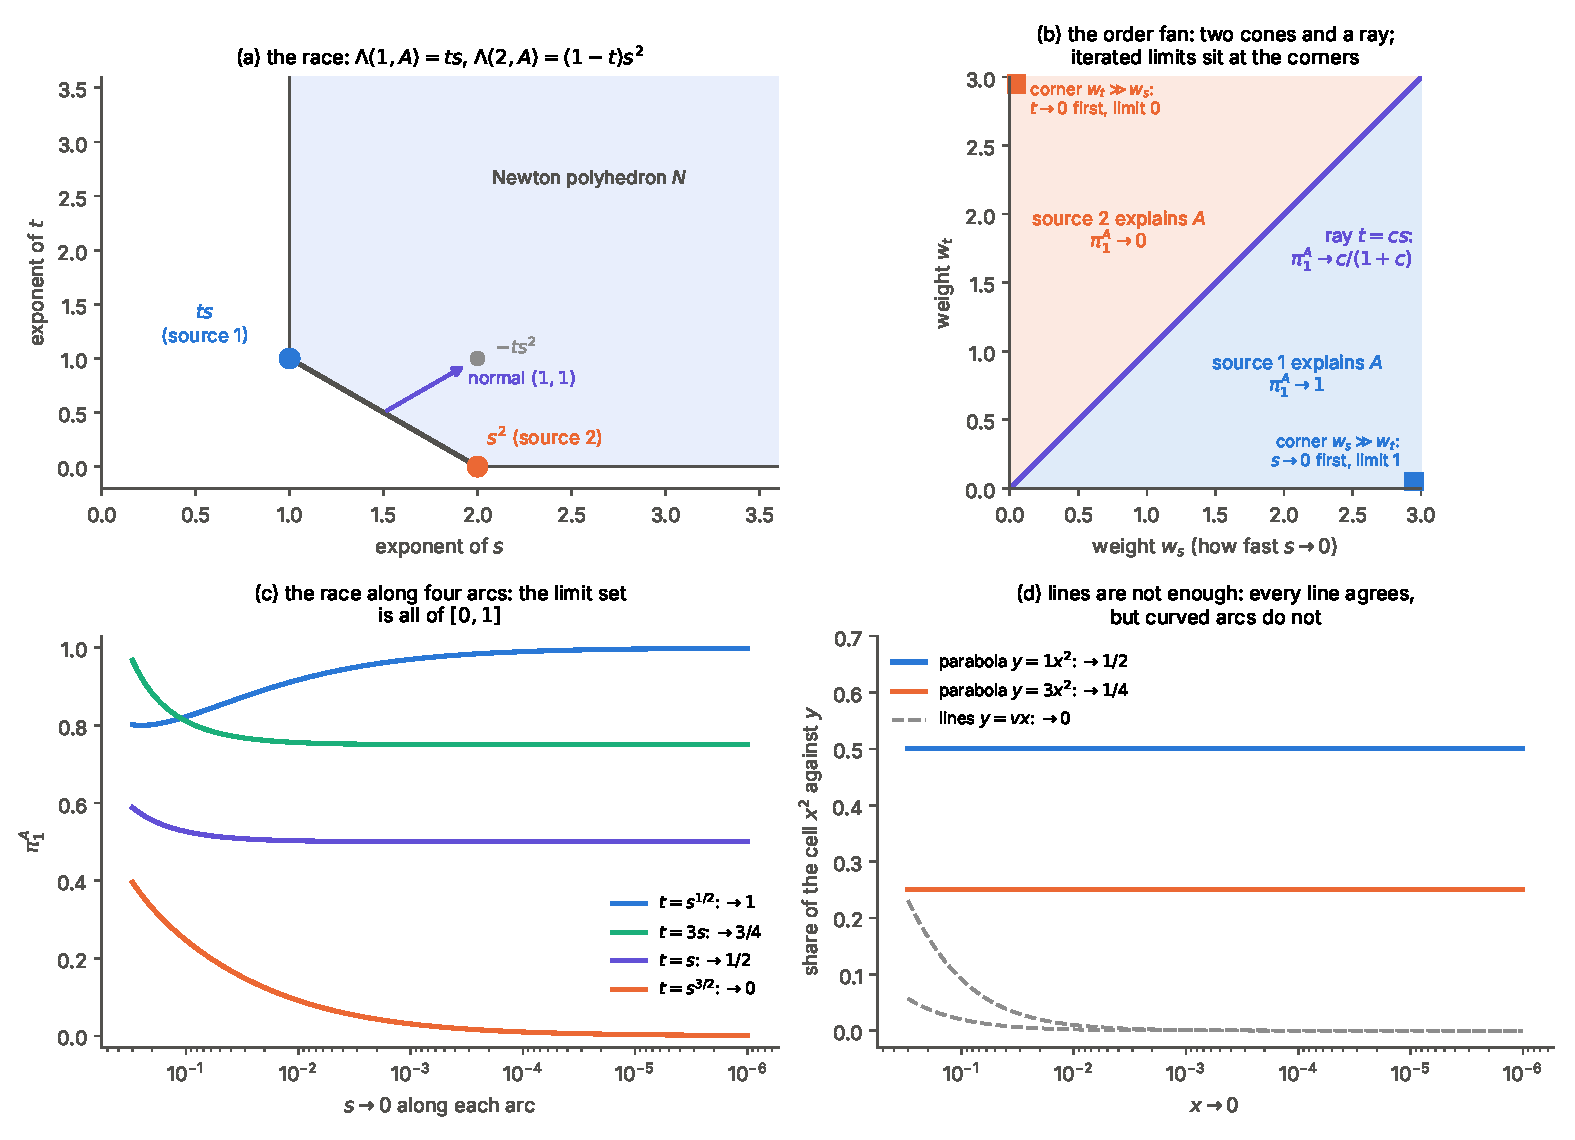
\includegraphics[width=\linewidth]{fig_fan.pdf}
\caption{Several parameters. (a) The Newton polyhedron of the race (\cref{ex:race}). (b) Its order fan: in each cone one source explains
$A$; on the ray both do, in proportion $c:1$; the iterated limits sit at the two corners (\cref{thm:iterated}). (c) The race along four
arcs, with four different limits. (d) \Cref{ex:curved}: every line gives $0$, every parabola something else.}\label{fig:fan}
\end{figure}

\section{Step 4b: iterated limits and the tangent tower}\label{sec:iterated}
Sending the parameters to $0$ one after another is an extreme way of moving through the fan: each parameter is infinitely smaller than
the next. This is exactly how the Weil algebra of Step 2 orders its generators, $e_1\ll e_2\ll\dots$. So the tangent tower computes
iterated limits, the corners of the fan, and the fan fills in everything between them.

\begin{theorem}[iterated limits are corners of the fan]\label{thm:iterated}
Fix an order $(i_1,\dots,i_d)$ and send $\varepsilon_{i_1}\to0$ with the others fixed, then $\varepsilon_{i_2}$, and so on. Each stage has a limit (for the parameters still held fixed, away from the zero set of a non-zero polynomial), and the
result is the normalised vector of coefficients at the lexicographic minimum $\alpha^\sigma$ of the exponents: minimise $\alpha_{i_1}$, then $\alpha_{i_2}$,
and so on. This $\alpha^\sigma$ is a vertex of $N$. The result equals the limit along any weight in the corner cone
$w_{i_1}\gg w_{i_2}\gg\dots\gg w_{i_d}$. Different orders can give different limits. If they all agree, the full limit can still fail to exist.
\end{theorem}

\begin{proof}
At the first stage every cell is a polynomial in $\varepsilon_{i_1}$ with coefficients in the other parameters. Its lowest power wins, with a
non-negative coefficient polynomial. Repeat. A lexicographic minimum minimises $\langle w,\cdot\rangle$ for sufficiently separated weights, so it is
a vertex. For the last claim, take $x^3+y^3$ (source $1$) against $xy$ (source $2$). Both iterated limits give source $1$, yet along $x=y$
source $2$ wins: the middle vertex $(1,1)$ of $N$ is seen by no corner. MP5 checks this exactly on $300$ families, all orders,
against the arc limit for super-increasing weights and against nested numerical evaluation.
\end{proof}

\begin{proposition}[the tower computes the corners]\label{prop:towerlex}
Let every cell be multilinear: exponents in $\{0,1\}^d$, as for a product $\pi_l(t)\,p_{l,s}(x)$ of a share and a likelihood, each moving in
its own parameter.
\begin{enumerate}
\item[(1)] The Weil point $\Lambda(e_1,\dots,e_d)$ lies in $T^d\Delta_{L\times X}$.
\item[(2)] The first monomial $e^S$, in the order of the lexicographic lemma, that carries mass on $L\times A$ gives, normalised, the iterated
  limit that sends $\varepsilon_1$ to $0$ first, then $\varepsilon_2$, and so on.
\item[(3)] The canonical flip $c$ of the tangent structure, which exchanges $e_1$ and $e_2$, gives the iterated limit in the other order.
\end{enumerate}
So the tangent tower sees exactly the corners of the order fan, and its flip moves between them. The cones in between, such as the ray
$t=cs$ of the race, are invisible to it. They need the fan.
\end{proposition}

\begin{proof}
(1) For each set $U$ of generators, setting the other parameters to $0$ keeps a cell non-negative. Along a super-increasing arc, its leading
coefficient is the first non-zero one in the lemma's order, so that coefficient is positive. (2) In the lemma's order $e^S$ precedes $e^{S'}$
iff the smallest generator of $S\triangle S'$ lies in $S'$. So monomials without $e_1$ come first, then, among those, monomials without $e_2$, and
so on: the lexicographic minimum of \cref{thm:iterated} with $\varepsilon_1$ first. (3) The flip is the substitution exchanging $e_1$ and $e_2$, that
is, exchanging the roles of $\varepsilon_1$ and $\varepsilon_2$. MP6 checks (1)--(3) on $200$ random multilinear families, $95$ of them with the flip.
\end{proof}

\begin{example}[two sources in the tower]\label{ex:tower2}
Source $1$'s share is $\varepsilon_1$ and source $2$'s likelihood of $A$ is $\varepsilon_2$. On $L\times A$ the Weil point has source $1$ on $e_1$ and
source $2$ on $e_2$. The lemma's order is $(1,e_2,e_1,e_1e_2)$. The first term with mass on $A$ is $e_2$, so source $2$ explains $A$: sending
the share $\varepsilon_1$ to $0$ first removes source $1$. The flip puts $e_1$ first, and source $1$ explains $A$. On the ray $\varepsilon_1=c\,\varepsilon_2$, between
the corners, the weights tend to $(\tfrac c{1+c},\tfrac1{1+c})$, which no point of $T^2$ records.
\end{example}

\begin{center}\small
\resizebox{\linewidth}{!}{\begin{tabular}{llllll}\toprule
example & cells on $L\times A$ & componentwise min & corners (iterated limits) & full limit & what it shows\\\midrule
\ref{ex:race} race & $ts$, $(1-t)s^2$ & none & $0$ and $1$ & none; limit set $[0,1]$ & a race between rarities\\
\ref{ex:dominance} dominance & $st$, $st+s^2t$ & $(1,1)$ & $\tfrac12$, $\tfrac12$ & $(\tfrac12,\tfrac12)$ & no race\\
\ref{ex:curved} curved path & $x^2$, $y$ & none & $0$ and $1$ & none, though every line gives $0$ & arcs, not lines\\
\ref{ex:degenerate} degenerate & $(x-y)^2$, $x^3$ & none & $1$ and $0$ & none; an interval inside one direction & refine the fan\\
\cref{thm:iterated} & $x^3+y^3$, $xy$ & none & $1$ and $1$ & none & corners are not enough\\
\ref{ex:tower2} tower & $\varepsilon_1$, $\varepsilon_2$ & none & $0$ and $1$ (the flip) & none & the tower sees corners only\\\bottomrule
\end{tabular}}
\end{center}

\emph{What this sets up.} The cross term $\sum_ld\pi_l\,dp_l$ of a pooled law, the target of Step 4d, is the coefficient of $e_1e_2$ when shares
move along $e_1$ and sources along $e_2$. It is a mixed order, read at the last place of the lemma's order. Step 4c will attach decisions
to the cones of the fan.

\section{Step 4c: parameters as an object, and decisions on the fan}\label{sec:para}
So far the parameters of Steps 3--4b were coordinates: a family was a map from a parameter space into the labelled simplex, and arcs were
chosen by hand. This section gives parameters their own place in the categorical picture, separate from both kinds of context already
in use. A \emph{measurement context} is a window of jointly observed variables, and a \emph{source} is the discrete label carried by $W$.
A \emph{parameter} is a quantity that moves and that drives a transition: a share, a rate, a design choice. It lives in a parameter space,
and changing how the parameters are described is a 2-cell. Decisions are then attached to the order fan, and they transport along those
2-cells.

\begin{definition}[parameterised source-indexed kernels]\label{def:para}
The 2-category $\mathrm{Para}_L$ has the finite sets as objects.
\begin{itemize}
\item A morphism $X\to Y$ is a pair $(P,f)$: a parameter space $P$ (here a semialgebraic subset of some $\R^d$) and a map
  $f:P\times L\times X\to\D Y$. For each parameter value it is a source-indexed kernel (\cref{prop:bikleisli}).
\item Composition is $(Q,g)\circ(P,f)=(P\times Q,\ (p,q,l,x)\mapsto\sum_yf(p,l,x)(y)\,g(q,l,y))$: parameters accumulate, and one source is
  held throughout.
\item A 2-cell $(P',f')\Rightarrow(P,f)$ is a \emph{reparametrisation}, a map $r:P'\to P$ with $f'=f\circ(r\times\mathrm{id})$.
\end{itemize}
This is the $\mathrm{Para}$ construction \cite{FongSpivakTuyeras2019,CruttwellEtAl2022} applied to the two-sided Kleisli category of $\lambda$.
A parameterised labelled law is a morphism $(P,\Lambda)$ from the one-point set into $L\times X$.
\end{definition}

\begin{proposition}[the layers act by post-composition]\label{prop:para}
\begin{enumerate}
\item[(1)] $\mathrm{Para}_L$ is a 2-category, strict once $(P\times Q)\times R$ is identified with $P\times(Q\times R)$. Reparametrisations whisker:
  $(g\circ f)\circ(r\times r')=(g\circ r')\circ(f\circ r)$.
\item[(2)] Labelling, pooling, marginalisation and forgetting provenance are parameter-free morphisms. Applying them after a
  reparametrisation equals reparametrising after applying them.
\item[(3)] Conditioning is partial. Its domain for $(P,\Lambda)$ is $\{p:\Lambda_p(L\times A)>0\}$, and that domain pulls back along every
  reparametrisation.
\end{enumerate}
So reparametrisation commutes with every layer operation at every parameter value. What it does not preserve is behaviour \emph{at the
boundary} of the parameter space. That behaviour is what the order fan describes, and reparametrisation can change which part of the fan
is reachable (\cref{ex:designs}).
\end{proposition}

\begin{proof}
(1) Composition of kernels with a fixed source is associative (\cref{prop:bikleisli}), and the parameters ride along as a product. Whiskering
is substitution. (2) Post-composition with a parameter-free morphism commutes with precomposition by $r$. (3) The domain condition is
evaluated pointwise. PR1 and PR2 check (1)--(3) exactly on random parameterised kernels and laws.
\end{proof}

\paragraph{Arcs are 2-cells; the germ field.} An arc into the corner of $P$ is a reparametrisation from the one-parameter germ line,
$s\mapsto\varepsilon(s)$. So Steps 3--4b classify such 2-cells by what happens at $s=0$. The same information sits in one algebraic object. Let
$\mathbb K=\R\{\!\{s\}\!\}$ be the field of real Puiseux series. It is a real closed ordered field, with valuation $v$ (the least exponent) and a
standard part $\operatorname{st}$ (the constant term of a bounded series). A Puiseux arc is a point $\varepsilon\in\mathbb K^d_{>0}$ with $v(\varepsilon_i)=w_i$ and
leading coefficients $c_i$. Evaluating the cells there gives a labelled law over $\mathbb K$. Its valuations are the tropical orders
$\operatorname{trop}_wf_c$ (off degenerate directions), and the standard part of its conditioned state is the arc limit of \cref{prop:arc} (PR3).
Sending parameters to $0$ one after another corresponds to nesting the fields, $\R\{\!\{s_1\}\!\}\{\!\{s_2\}\!\}\cdots$. These are the corners of the fan
(\cref{thm:iterated}). For multilinear cells no squares occur, so the Weil algebra of Step 2 already suffices (\cref{prop:towerlex}).

\paragraph{Decisions.} A decision problem is a finite set of acts with utilities $u_a$ on $L\times X$. The act chosen at a parameter value
maximises $\langle u_a,\Phi(\varepsilon)\rangle$, the expected utility under the conditioned state. Along an arc, the comparison of $a$ and $b$ is
the germ $D_{ab}(s)=\langle u_a-u_b,\Phi(\varepsilon(s))\rangle$, an element of $\mathbb K$.

\begin{theorem}[the decision fan]\label{thm:decisionfan}
\begin{enumerate}
\item[(1)] Along every Puiseux arc the optimal act is eventually constant. It is decided in the ordered field $\mathbb K$ by the sign of the
  leading coefficient of each $D_{ab}$. A comparison is undecided only if $D_{ab}\equiv0$, a genuine tie along the whole arc.
\item[(2)] If the limiting state $\operatorname{st}\Phi$ has a unique optimal act, the eventual act is that act. If the limiting state has a tie, the
  next order of $D_{ab}$ breaks it.
\item[(3)] On a cone of the order fan that belongs to a vertex of $N$, the limiting state is fixed, so the limiting act is constant there. A
  cone that belongs to an edge or a higher face is cut further by the walls $\langle u_a-u_b,\operatorname{in}_F f(c)\rangle=0$, which are polynomial in
  the arc coefficients $c$.
\item[(4)] \emph{Transport.} Let $r(\delta)=\delta^R$ be a monomial reparametrisation, $\varepsilon_i=\prod_j\delta_j^{R_{ij}}$. Then the arc $(w',c')$ in the new parameters
  maps to the arc $(Rw',c'^R)$ in the old ones. Arc limits and eventual acts are pulled back: the order fan and the decision fan of
  $\Lambda\circ r$ are the preimages of those of $\Lambda$ under $w'\mapsto Rw'$.
\end{enumerate}
\end{theorem}

\begin{proof}
(1) Each $D_{ab}$ is a ratio of Puiseux series in $s$ with a positive denominator, so it is $0$ or eventually of the sign of its leading
coefficient. Finitely many comparisons decide the act. (2) $\operatorname{st}D_{ab}$ is the limiting comparison; if it is $0$, the leading coefficient lies
at a higher order. (3) This is \cref{thm:fan}(2) composed with a linear functional. (4) $\delta_j=c'_js^{w'_j}$ gives
$\varepsilon_i=\prod_jc'^{R_{ij}}_js^{\sum_jR_{ij}w'_j}$; then apply \cref{prop:para}(2). PR4 checks (1)--(2) on $300$ random families and utilities,
including $49$ ties at the limit broken at higher order, against evaluation at $s=10^{-8}$. PR6 checks (4) on $200$ random reparametrisations.
\end{proof}

\begin{example}[which source to audit]\label{ex:audit}
In the race of \cref{ex:race}, a flagged record arrives and one source is to be audited. Auditing the source that produced the record pays $1$;
auditing the other pays $0$. The optimal act audits the source with the larger posterior weight. The decision fan
(\cref{fig:para}(a)) is:
\begin{itemize}
\item when the share vanishes more slowly than the event rate ($w_t<w_s$), audit the small trials (source $1$);
\item when it vanishes faster ($w_t>w_s$), audit the registry (source $2$);
\item on the ray $t=cs$, audit source $1$ iff $c>1$, and source $2$ iff $c<1$;
\item at $c=1$ the limiting state is $(\tfrac12,\tfrac12)$, a tie. The comparison germ is $D_{12}(s)=s^3/(\text{positive})$, from the factor $1-t$ in the
  registry's cell, so the next order decides: audit source $1$ (PR5).
\end{itemize}
The tie at the limit is broken by a term that no first-order analysis sees. This is a third-order effect deciding a first-order question.
\end{example}

\begin{example}[two study designs are two reparametrisations]\label{ex:designs}
The same two sources can be studied under different designs. Each design is a reparametrisation of $(s,t)$, a 2-cell into the race.
\begin{itemize}
\item \emph{Design 1}, $t=s\,u$: the small-trial share is set in proportion to the event rate. The weights become $w=(w_s,\ w_s+w_u)$, which is exactly the
  cone $w_t>w_s$. The exponents of $\Lambda\circ r$ have the componentwise minimum $(2,0)$, so the limit exists. By every route to the corner,
  the registry explains a flagged record: audit source $2$.
\item \emph{Design 2}, $s=u\,v$ and $t=u$: the event rate is tied to the share. The weights become $w=(w_u+w_v,\ w_u)$, the cone $w_s>w_t$. The
  componentwise minimum is $(2,1)$, the limit exists, and the small trials explain the record: audit source $1$.
\end{itemize}
In the raw parameters the race has no limit at all (\cref{ex:race}). Each design fixes the race in advance by occupying one cone of the
fan, and \cref{thm:decisionfan}(4) transports the decision along the 2-cell (\cref{fig:para}; PR6). A design that sits on the ray, such as $t=s\,(1+u)$,
ends in the tie $(\tfrac12,\tfrac12)$. There the comparison $ts-(1-t)s^2=s^2u+s^3(1+u)$ is positive, so it audits source $1$ by every route.
\end{example}

\begin{figure}[!htbp]\centering
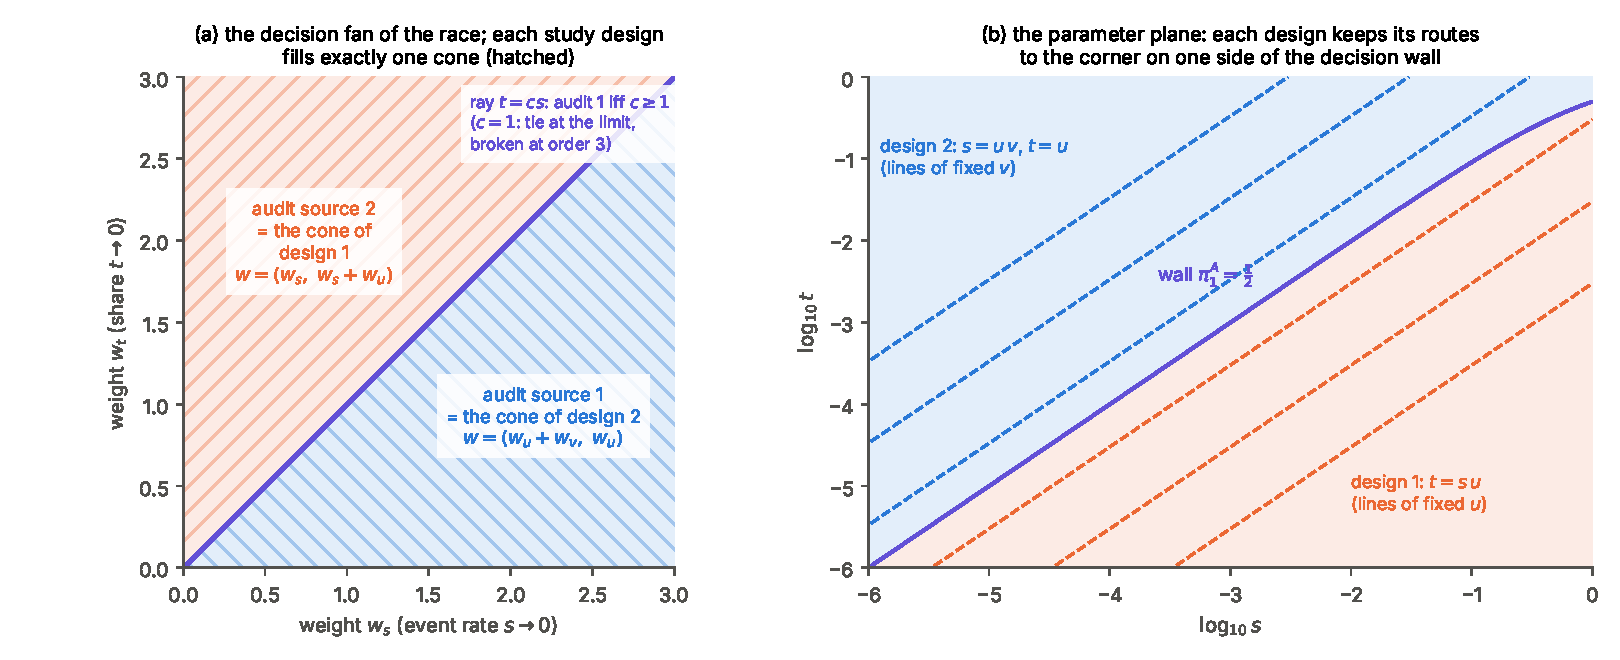
\includegraphics[width=\linewidth]{fig_para.pdf}
\caption{Step 4c on the race. (a) The decision fan of \cref{ex:audit}. Each design of \cref{ex:designs} fills one cone exactly. (b) The
parameter plane on log scales, with the decision wall $\pi^A_1=\tfrac12$. The routes of design $1$ (lines of fixed $u$) and design $2$ (lines
of fixed $v$) stay on opposite sides.}\label{fig:para}
\end{figure}

\emph{What this sets up for Step 4d.} The cross term $\sum_ld\pi_l\,dp_l$ is the coefficient of $e_1e_2$ when the shares move along one parameter and
the sources along another. Here that means the mixed order of the comparison germ on the diagonal cone of the share--likelihood fan. The
graded classes of maps and the contextual second-order theorem will be stated in this setting.

\section{Step 4d: the decorated fan, the cross term, and Theorem J}\label{sec:stat}
This step does three things.
\begin{itemize}
\item It separates the two levels of information in the order fan, in the probability-decorated order fan: the geometry, which says which exponents can dominate, and the
  probability carried on each cone, which says which sources survive and with what weights.
\item It isolates the cross term $\sum_la_l\,u_l$ of pooling exactly.
\item It derives the band of the lab's Theorem J \cite[Theorem J]{Lab} as an inequality between orders on a \emph{statistical} fan, in which the
  sample size is one more parameter, and it marks the cones where J's Gaussian bands are valid and where they are not.
\end{itemize}

\subsection{The probability-decorated order fan}
\begin{definition}[probability-decorated order fan]\label{def:decorated}
A \emph{probability-decorated order fan} consists of a geometric Newton fan together with compatible facewise initial-form data, which
determine the limiting conditioned laws. For cells $(f_c)$ on $L\times A$ it is the pair $(\Sigma_N,\mathcal O)$:
\begin{itemize}
\item $\Sigma_N$ is the geometric fan of \cref{thm:fan}, with one cone $\sigma_F$ for each bounded face $F$ of $N$;
\item $\mathcal O$ is the \emph{facewise presheaf of initial forms}. It is the functor on the poset of bounded faces of $N$, ordered by inclusion,
  that sends $F$ to the tuple of face parts $(f^F_c)_c$, the monomials of each cell with exponents in $F$. A face $G\subseteq F$ gets the
  restriction $\rho_{F,G}:f^F\mapsto(f^F)^G$.
\end{itemize}
The decoration on $F$ determines the \emph{limit map} $\ell_F(c)=\text{normalise}\bigl(f^F_c(c)\bigr)_c$ on the cone of $F$. A \emph{decision
decoration} adds the comparison functionals $\langle u_a-u_b,\ell_F(c)\rangle$ of \cref{thm:decisionfan}.
\end{definition}

\begin{proposition}[the facewise presheaf of initial forms]\label{prop:decorated}
\begin{enumerate}
\item[(1)] The restrictions compose, $(f^F)^G=f^G$ for $G\subseteq F$, so $\mathcal O$ is a presheaf on the face poset. In terms of weights,
  $\operatorname{in}_{w'}(\operatorname{in}_wf)=\operatorname{in}_{w+\epsilon w'}f$ for all small $\epsilon>0$.
\item[(2)] Along an edge $F=[\alpha,\beta]$, if no initial form vanishes, the limit map tends to the vertex limit $\ell_\alpha$ as
  $c^{\beta-\alpha}\to0$ and to $\ell_\beta$ as $c^{\beta-\alpha}\to\infty$. So the limit set over an edge is a path joining the limits of its two vertices.
\item[(3)] The geometric fan does not determine the limits. Two decorations of the same Newton polyhedron can have different limit sets.
\end{enumerate}
\end{proposition}

\begin{proof}
(1) The monomials of $f$ that minimise $\langle w,\cdot\rangle$ and then, among those, $\langle w',\cdot\rangle$ are those that minimise
$\langle w+\epsilon w',\cdot\rangle$ for small $\epsilon$. (2) On $F$ every exponent is $\alpha+t(\beta-\alpha)$ with $t\in[0,1]$, so $f^F(c)=c^\alpha\sum_ta_t(c^{\beta-\alpha})^t$, and
the lowest or highest $t$ dominates. (3) Take cells $x$ (source $1$) and $y$ (source $2$), against $x+y$ (source $1$) and $x$ (source $2$).
Both have the Newton polyhedron with vertices $(1,0)$ and $(0,1)$. Along $y=cx$, the first gives $\pi^A_1=\tfrac1{1+c}$, filling $[0,1]$. The
second gives $\pi^A_1=\tfrac{1+c}{2+c}$, filling only $[\tfrac12,1]$ (\cref{fig:stat}(d)). ST1 checks (1)--(2) exactly on random families and $53$
edges; ST2 checks (3).
\end{proof}

So the fan says which exponents can dominate, and the decoration says which sources survive and with what weights. Only the pair
determines the limiting conditioned law.

\begin{remark}[why ``presheaf'' and not ``sheaf'']
Proposition~\ref{prop:decorated}(1) gives a coherent restriction system, a presheaf, and nothing in this paper uses a gluing property. A
sheaf needs a topology and gluing. One can supply both: give the face poset its Alexandrov topology, whose open sets are the sets of faces
closed under passing to subfaces. On a finite poset, presheaves for this topology extend uniquely to sheaves, the \emph{cellular sheaves} of
\cite{Curry2014}, and gluing and uniqueness then hold automatically. Moreover $\mathcal O$ has a canonical global section, the cells themselves,
from which every local section is obtained by restriction. We keep the safer name, \emph{facewise presheaf}, because the content of the
proposition is (3), not gluing.
\end{remark}

\subsection{The cross term of pooling}
\begin{proposition}[the cross term]\label{prop:cross}
\begin{enumerate}
\item[(1)] Pooling is exactly bilinear:
  $\mu_n(\pi+a,p+u)-\mu_n(\pi,p)=\sum_la_lp_l+\sum_l\pi_lu_l+\sum_la_lu_l$.
\item[(2)] With the shares moving along $e_1$ and the sources along $e_2$, the coefficient of $e_1e_2$ is the cross term $\sum_la_lu_l$. The
  second-order coefficients of a move along shares alone, or along sources alone, vanish. The cross term is the whole curvature of pooling.
\item[(3)] After conditioning, the mixed second derivative of $C_A\circ\mu_n$ goes through the Bayes weights:
  \[
  \partial_a\partial_u(C_A\circ\mu_n)=\sum_l\partial_a\partial_u\pi^A_l\,C_A(p_l)+\sum_l\partial_a\pi^A_l\,DC_A(p_l)[u_l].
  \]
\item[(4)] On a fan where the shares move at order $w_a$ and the sources at order $w_u$, the cross term has order $w_a+w_u$ (\cref{thm:tropical}).
\end{enumerate}
\end{proposition}

\begin{proof}
(1) Expand. (2) is (1) in $W_2$. (3) Differentiate \cref{thm:bayes}; $C_A(p_l)$ does not depend on $a$. (4) A product of germs. ST3 checks
(1)--(3), (1) exactly and (2)--(3) in the Weil algebra against the explicit formula.
\end{proof}

\subsection{Theorem J on a statistical fan}
\paragraph{Statistical assumptions.} The statements of this subsection and the next hold under the following assumptions, which are
those of J \cite[Theorem J]{Lab} made explicit.
\begin{itemize}
\item[(S1)] Records are independent. The share $\pi$ of source $C$ and the genuine law are fixed by design, not estimated.
\item[(S2)] \emph{Gaussian model} (\cref{thm:Jfan}). Each source statistic is normal with known variance $\sigma^2$, exactly or as the large-count
  limit. This requires the relevant counts to grow, that is, to lie in the Gaussian cone of \cref{prop:poisson}.
\item[(S3)] \emph{Poisson model} (\cref{thm:poissonband}). Flags, the records falling in a rare event $A$, arrive as independent Poisson counts.
  This is exact for a Poisson process of records, and it is the rare-event limit of binomial counts.
\item[(S4)] The adversary is deterministic: it chooses its share and its shift (or its flag rate) in advance, and only raises them.
\item[(S5)] The exposure test and its level are fixed before the data. Arcs are taken along $N\to\infty$, with every parameter a germ in a Hardy field
  (in practice, a power of $s=N^{-1/2}$).
\end{itemize}

Recall the setting of J \cite[Theorem J]{Lab}, which uses a Gaussian model:
\begin{itemize}
\item source $C$ holds a share $\pi$ of $N$ records, and its records' statistic is shifted by $D$;
\item its source statistic has mean $a=D\sqrt{\pi(1-\pi)N}/\sigma$;
\item the pooled estimate moves by $\pi D$, which is $I=\pi D\sqrt N/\sigma$ pooled standard errors.
\end{itemize}
Pooling with a new source is a move from the corner $\pi=0$ of the share simplex, so the impact $\pi D$ is precisely the cross term of
\cref{prop:cross}: share times shift. Now treat the sample size as a parameter of $\mathrm{Para}_L$: $s=N^{-1/2}$, the share $\pi\sim p\,s^{w_\pi}$, and
the shift $D\sim d\,s^{w_D}$.

\begin{theorem}[Theorem J as an inequality of orders]\label{thm:Jfan}
Along any such arc:
\begin{enumerate}
\item[(1)] $I=a\sqrt{\pi/(1-\pi)}$ exactly. The orders are $v(a)=w_D+w_\pi/2-1$ and $v(I)=w_\pi+w_D-1$. The impact counts the share at full
  weight, and the exposure only at half weight.
\item[(2)] \emph{The regimes are cones.} Below the exposure line $w_D+w_\pi/2=1$, $a\to\infty$ and $C$ is exposed with probability tending to $1$.
  Above it, $a\to0$ and the exposure rate falls to the false-alarm rate. On the line, the exposure probability tends to
  $1-\Phi(c_s-a_0)$, with $a_0$ the leading coefficient of $a$.
\item[(3)] \emph{The band.} Bounded exposure, $P(\text{exposed})\le\beta$, means $a\le a_{\max}=c_s-\Phi^{-1}(1-\beta)$. That forces $w_D+w_\pi/2\ge1$, hence
  $v(I)\ge w_\pi/2\ge0$, and
  \[
  I\le a_{\max}\sqrt{\pi/(1-\pi)}=B .
  \]
  The impact stays of order one only at the single point $(w_\pi,w_D)=(0,1)$: a fixed share, with a shift shrinking like $N^{-1/2}$. That is
  J(2). If the share also vanishes ($w_\pi>0$), the impact vanishes like $s^{w_\pi/2}$.
\item[(4)] \emph{No tilt.} Under bounded exposure the raw pooled shift $\pi D$ has order $w_\pi+w_D\ge1+w_\pi/2>0$, so it tends to $0$ and cannot cross a
  fixed settling radius. The adversary that does tilt the pooled decision, with fixed share and fixed shift ($w_\pi=w_D=0$), lies in the
  exposed cone. This is the limiting content of J(3).
\end{enumerate}
\end{theorem}

\begin{proof}
(1) J's identity \cite[proof of Theorem J(2)]{Lab}, with $v$ applied through \cref{thm:tropical}. (2) The source statistic is normal with mean $a$
and variance $1$. (3) Monotonicity of $\Phi$, then (1). (4) A product of germs. ST4 checks the orders as slopes on log scales and the bound at
three sample sizes and three shares. ST5 checks (2) by Monte Carlo along three arcs at $N=10^3,10^4,10^5$: the exposure rate rises to $1$,
stays at $1-\Phi(c_s-a_0)\approx0.095$ on the line, and falls to the false-alarm rate $0.023$.
\end{proof}

So J's band is the leading coefficient of the cross term on the one ray of the statistical fan where exposure is of order one. The band
exists because exposure sees the share at half weight ($\sqrt\pi$), while the impact sees it at full weight (\cref{fig:stat}(a)). This
answers the question left open in the scope of Steps 1--3, for J's Gaussian model.

\subsection{Where Gaussian bands are valid}
J's bands are Gaussian, and Gaussian approximations need counts that grow. The order fan says when they do. Let an event have
probability $P(A)\sim c\,s^{w_A}$, again with $s=N^{-1/2}$. Its expected count is $c\,s^{w_A-2}$.

\begin{proposition}[the Gaussian cone, the Poisson ray, and the empirical wall]\label{prop:poisson}
\begin{enumerate}
\item[(1)] If $w_A<2$, the count grows, conditional estimates such as $\hat\pi^A_l$ are asymptotically normal, and Wald bands are
  asymptotically valid.
\item[(2)] If $w_A=2$, the count tends to $\mathrm{Poisson}(c)$. There is no event with probability $e^{-c}$, and conditional estimates have a discrete
  limiting law, so Gaussian bands are not valid. In ST6, with $c=3$ and $\pi^A_1=0.3$, the nominal $95\%$ interval covers about $50\%$ at every $N$.
\item[(3)] If $w_A>2$, there is no event with probability tending to $1$. The empirical conditional is undefined: an \emph{empirical wall}, the
  sample-level analogue of \cref{prop:wall}.
\end{enumerate}
The same split applies to source $C$'s own record count $\pi N$. J's Gaussian derivation needs $w_\pi<2$. On the ray $w_\pi=2$, C contributes a
bounded number of records, and its source statistic is no longer normal.
\end{proposition}

\begin{proof}
The law of rare events for $w_A=2$, the central limit theorem when the count grows, and $P(\text{no event})=(1-P(A))^N$. ST6 simulates all three
cases at $N=10^2,10^4,10^6$. ST7 is the negative control: the same procedure at a fixed $P(A)=0.2$ covers within Monte Carlo error once $N\ge10^4$.
At $N=100$ the Wald interval already under-covers (about $0.92$), a known small-sample effect.
\end{proof}

\subsection{A band on the Poisson ray}
On the Poisson ray the source statistic is a count, and J's normal approximation fails. An exact discrete band replaces it. Under (S3), let
$C$ produce $X_C\sim\mathrm{Poisson}(\mu_C)$ flags and the genuine sources $X_O\sim\mathrm{Poisson}(\mu_O)$. Under the null, $C$ flags at the genuine rate, so
$\mu_C=\mu_0=\pi\mu_O/(1-\pi)$. Use the \emph{exact conditional test}: given $T=X_C+X_O$, under the null $X_C\sim\mathrm{Binomial}(T,\pi)$, and the test rejects
when $X_C\ge k_\alpha(T)$. Here $k_\alpha(T)$ is the least $k$ with $P(\mathrm{Bin}(T,\pi)\ge k)\le\alpha$, or $T+1$ if there is none. The adversary's excess is
$\Delta=\mu_C-\mu_0$ expected flags. In pooled standard errors this is $\Delta/\sqrt{Np}$, where $Np=\mu_O/(1-\pi)$ is the genuine pooled flag mean.

\begin{theorem}[the band on the Poisson ray]\label{thm:poissonband}
\begin{enumerate}
\item[(1)] \emph{Exact band.} $k_\alpha(T+1)\le k_\alpha(T)+1$, so the rejection region grows with $X_C$. The exposure probability is therefore increasing in
  $\mu_C$, and it is at most $\alpha$ under the null. An adversary with exposure at most $\beta$ adds at most
  \[
  \Delta_{\max}(\mu_O)=\mu_C^{\max}-\mu_0\ \text{expected flags},\qquad B_{\mathrm{pois}}=\Delta_{\max}/\sqrt{Np}\ \text{pooled standard errors},
  \]
  where $\mu_C^{\max}$ is the exposure-$\beta$ point. This holds at every count, with no normal approximation.
\item[(2)] \emph{Gaussian limit.} As $\mu_O\to\infty$ (the Gaussian cone), $B_{\mathrm{pois}}\to B=\bigl(\Phi^{-1}(1-\alpha)-\Phi^{-1}(1-\beta)\bigr)\sqrt{\pi/(1-\pi)}$. This is J's band.
\item[(3)] \emph{The Poisson ray.} At bounded $\mu_O$, $B_{\mathrm{pois}}$ is a fixed number above $B$. The test also has a \emph{blind spot}: with
  $t_b=\lceil\log\alpha/\log\pi\rceil-1$, it cannot reject at all when $T\le t_b$, whatever the adversary does.
\item[(4)] \emph{The wall side.} As $\mu_O\to0$, $\Delta_{\max}\to\lambda^*$, where $P(\mathrm{Poisson}(\lambda^*)\ge t_b+1)=\beta$. The band in standard errors diverges,
  so standard errors are the wrong unit there, and counts are the right one. The adversary's expected share of the flags tends to $1$: an
  exposure-bounded adversary \emph{owns} the rare event, and by \cref{thm:hierarchy} it explains it in the conditioned law.
\end{enumerate}
\end{theorem}

\begin{proof}
(1) $\mathrm{Bin}(T,\pi)+\mathrm{Bern}(\pi)\ge k+1$ implies $\mathrm{Bin}(T,\pi)\ge k$, so $k_\alpha(T+1)\le k_\alpha(T)+1$. Hence, for fixed $X_O$, the rejection set is
upward closed in $X_C$, and $X_C$ is stochastically increasing in $\mu_C$. Under the null the conditional test has level $\alpha$ given every $T$.
Exposure is computed exactly by Poisson splitting: $T\sim\mathrm{Poisson}(\mu_C+\mu_O)$, and given $T$, $X_C\sim\mathrm{Bin}(T,\mu_C/(\mu_C+\mu_O))$.
(2) The conditional statistic $(X_C-T\pi)/\sqrt{T\pi(1-\pi)}$ has mean $\approx\Delta\sqrt{1-\pi}/\sqrt{Np\,\pi}$, so the impact is that mean times
$\sqrt{\pi/(1-\pi)}$, as in \cref{thm:Jfan}(1). Then use the central limit theorem.
(3) $k_\alpha(T)=T+1$ iff even $X_C=T$ is not rare enough, that is, iff $\pi^T>\alpha$, that is, iff $T\le t_b$.
(4) $X_O=0$ with probability tending to $1$. Then $T=X_C$, and the test rejects iff $X_C\ge t_b+1$.
Checks: PB1 checks (1) for $T<3000$ and three values of $\mu_O$. PB2 checks exposure $=\beta$ at the band, against $200{,}000$ Monte Carlo draws.
PB3 checks (2): $B_{\mathrm{pois}}=0.389,0.283,0.250,0.238$ at $\mu_O=10,10^2,10^3,10^4$, against $B=0.2325$. PB4 checks (3): $t_b=3$, and at $\mu_O=3$ the band is
$0.636$ standard errors, $2.74\,B$. PB5 checks (4): $\lambda^*=1.366$ flags, with share $0.9993$ at $\mu_O=10^{-3}$.
\end{proof}

So on the Poisson ray an adversary can move the pooled estimate almost three times further, in standard errors, than J's Gaussian band
allows. Beyond the ray, a bounded number of injected flags becomes the whole explanation of the event (\cref{fig:graded}(a)). This
closes the Poisson case under (S1), (S3)--(S5).

\begin{figure}[!htbp]\centering
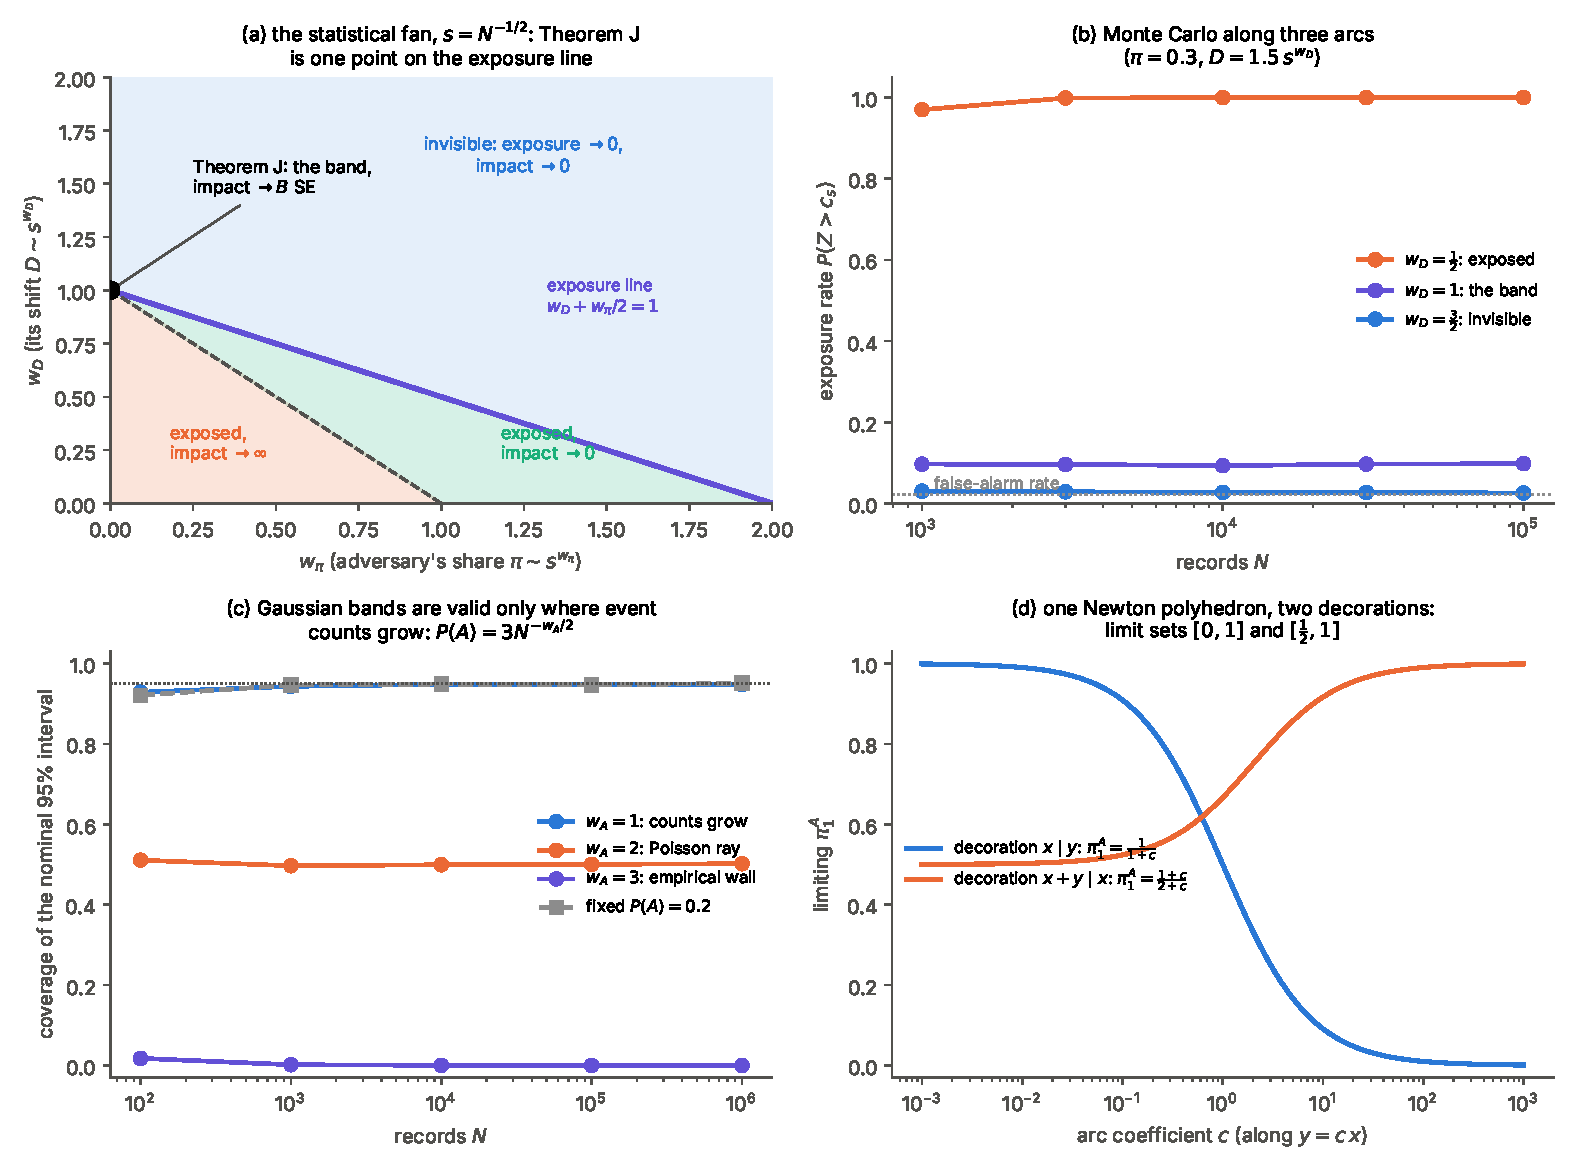
\includegraphics[width=\linewidth]{fig_stat.pdf}
\caption{Step 4d. (a) The statistical fan in the share and shift orders, with $s=N^{-1/2}$. Theorem J is the point $(0,1)$ on the exposure line
(\cref{thm:Jfan}). (b) Monte Carlo exposure rates along three arcs. (c) Coverage of nominal $95\%$ Wald intervals: valid where counts grow,
failing on the Poisson ray, and undefined beyond it (\cref{prop:poisson}). (d) One Newton polyhedron with two decorations
(\cref{prop:decorated}(3)).}\label{fig:stat}
\end{figure}

\emph{What is proved, and what is not.} Under (S1), (S2), (S4) and (S5), the band, the vanishing-share extension and the no-tilt limit follow
from the order calculus and the cross term. Under (S1), (S3)--(S5), the exact discrete band of \cref{thm:poissonband} covers the Poisson ray
and the wall side. A band for decisions that depend on the decoration near the walls is open.


\section{Step 4e: graded classes of maps}\label{sec:graded}
Steps 2--4 kept asking one question of each map: does it keep feasibility at order $k$? This section names the answer and shows that every
layer operation passes at every order. It also locates exactly what fails: subtraction.

\begin{definition}[graded classes]\label{def:graded}
For $1\le k\le\infty$, $\mathcal M_k$ is the class of smooth maps $f$ between products of simplices, partial maps on relatively open domains
included, such that $T^kf$ maps $T^k$ of the domain into $T^k$ of the codomain at every point of the domain. ($\mathcal M_\infty=\bigcap_k\mathcal M_k$.) A map is
\emph{subtraction-free} if each output cell is built from the input coordinates and positive constants by sums, products, and division by
expressions that are positive on the domain.
\end{definition}

\begin{theorem}[the graded classes]\label{thm:graded}
\begin{enumerate}
\item[(1)] Each $\mathcal M_k$ is a subcategory, and $\mathcal M_1\supseteq\mathcal M_2\supseteq\mathcal M_3\supseteq\cdots\supseteq\mathcal M_\infty$.
\item[(2)] The first two inclusions are strict:
  \begin{itemize}
  \item $q\mapsto(1-(q_1-q_2)^2,(q_1-q_2)^2,0)$ lies in $\mathcal M_1$ but not in $\mathcal M_2$;
  \item $q\mapsto(1-g,g,0)$ with $g=x_1(x_1-x_2)^2$ lies in $\mathcal M_2$ but not in $\mathcal M_3$.
  \end{itemize}
\item[(3)] Every subtraction-free map lies in $\mathcal M_\infty$.
\item[(4)] Consequently every layer operation lies in $\mathcal M_\infty$ on its domain:
  \begin{itemize}
  \item stochastic matrices, $\lambda$, $\D\epsilon$ and the marginalisations $M_S$;
  \item pooling $\mu_n$, the labelled joint $J$ and products of laws;
  \item conditioning $C_A$ and the labelled conditioning $\mathfrak C_A$;
  \item the Bayes-weight map $(\pi,p)\mapsto\pi^A$ and the Bayesian inverse $K^\dagger$.
  \end{itemize}
  In particular, conditioning keeps feasibility at every order. This settles the question left open in Step 2, which went only as far as order two.
\end{enumerate}
\end{theorem}

\begin{proof}
(1) $T^k$ is a functor. The zero section $T^k\to T^{k+1}$ (zero coefficients on monomials containing $e_{k+1}$) preserves and reflects
membership, because in the lexicographic lemma it interleaves each sequence with zeros. So if $T^{k+1}f$ preserves $T^{k+1}$, then $T^kf$
preserves $T^k$.
(2) The first map is the counterexample of \cite[Proposition ``morphisms'']{TangentCompanion}. The second is the order-three example of
\cite[Proposition ``order $k$: necessity, and order three'']{TangentCompanion}, which passes the second-order criterion.
(3) $T^kf$ evaluates the same expression in the Weil algebra $W_k$. The input cells lie in $T^kH$. $T^kH$ is a convex cone, so it is closed under
sums and positive multiples, and it is closed under products by \cref{thm:tensor}. A Weil number with positive constant term lies in $T^kH$
(every lexicographic sequence starts with a positive entry), and so does its inverse, whose constant term is the inverse of a positive
number. So every output cell lies in $T^kH$. The output equations ($\sum_y f_y=1$ and zero sums for the higher coefficients) hold because a
rational identity on the domain holds in $W_k$ wherever its denominators are invertible.
(4) Each listed map is subtraction-free on its domain. For example, $C_A(p)(x)=p(x)\cdot\bigl(\sum_{x'\in A}p(x')\bigr)^{-1}$ with $p(A)>0$, and
$\pi^A_l=\pi_lp_l(A)/\sum_j\pi_jp_j(A)$.
Checks: GC1 checks the zero section; GC2 and GC3 check the separations by direct $T^2$ and $T^3$ sampling. GC4 checks units and inverses
for $k\le4$. GC5 checks (3)--(4) on $2300$ sampled points of $T^3$ and $T^4$ at corners, for conditioning, the labelled conditioning, the
Bayes weights, the Bayesian inverse, products, and random normalised positive polynomial maps.
\end{proof}

\begin{remark}[where feasibility breaks]
\Cref{thm:graded}(3) says that, within the layers, only subtraction can take a map out of $\mathcal M_k$. Both separating examples square a
contrast $q_1-q_2$. GC6 finds that every one of $40$ random maps carrying the square of a contrast leaves $\mathcal M_2$ at the vertex. In the lab,
contrasts are exactly the estimators: covariances, tetrads, the decision gap $U_T-U_P$. This is why the curvature that produces the
pooling paradox \cite[Proposition ``pooling paradox = curvature'']{TangentCompanion} lives in the decision functional and never in a layer
operation (\cref{fig:graded}(b)). The converse fails: at relative-interior points every smooth map lies in every $\mathcal M_k$, so $\mathcal M_\infty$ is
much larger than the subtraction-free maps. The graded classes are about boundaries.
\end{remark}

\begin{figure}[!htbp]\centering
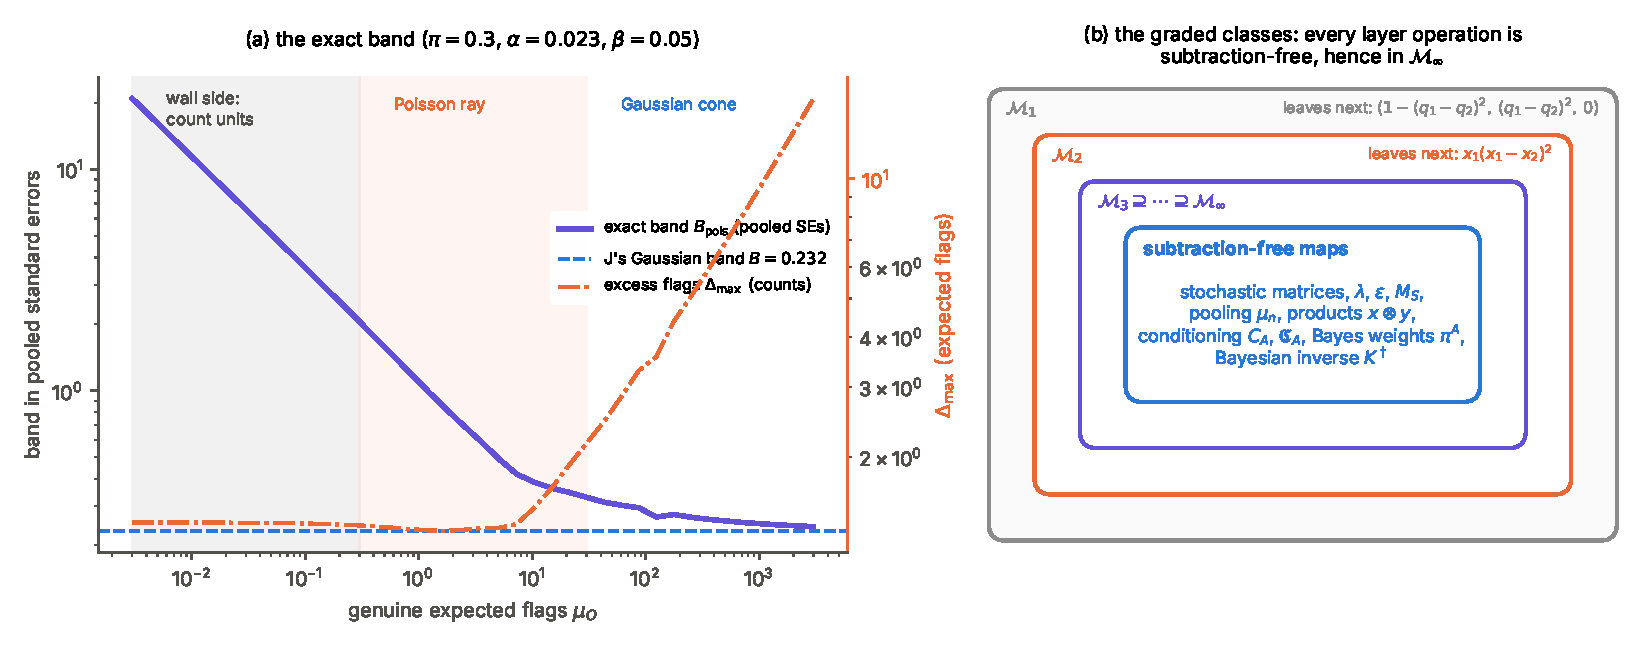
\includegraphics[width=\linewidth]{fig_graded.pdf}
\caption{(a) The exact band of \cref{thm:poissonband} in pooled standard errors (left axis) and in expected flags (right axis). It falls to J's
Gaussian band $B$ in the Gaussian cone, stays well above it on the Poisson ray, and diverges in standard-error units on the wall side, where
the count $\Delta_{\max}\to\lambda^*\approx1.37$ is the right measure. (b) The graded classes (\cref{thm:graded}).}\label{fig:graded}
\end{figure}

\emph{Next.} The degenerate directions of \cref{thm:fan}(5) are resolved in Step 4f (\cref{thm:degen}).

\section{Step 4f: degenerate directions, recursively}\label{sec:degen}
\Cref{thm:fan}(5) left one gap. Along a direction where the initial forms vanish, the leading terms say nothing, and the next terms of the
arc decide. \Cref{ex:degenerate} showed a whole interval of limits hidden inside a single direction. This section shows how to resolve such
directions, recursively and in finitely many steps, for two parameters.

The key simplification is this. A direction needs refining only when the initial forms of \emph{all} the least-order cells vanish. If
only some vanish, those cells drop out and the others give the limit at once (\cref{prop:arc}). Every cell is non-negative, so their
initial forms are non-negative at the arc coefficient and cannot cancel. So all of them vanish exactly when the initial form of their
sum $P(A)=\sum_cf_c$, the event's total mass, vanishes. Degeneracy is therefore a property of one polynomial, $P(A)$, and resolving it is the
classical Newton--Puiseux algorithm for that polynomial \cite{Walker1950,CasasAlvero2000}. The cells only decorate the result.

\paragraph{Setting.} There are two parameters $(x,y)\to0$ in the open quadrant. The cells $f_c\in\R[x,y]$ on $L\times A$ are non-negative there, and
$P(A)\not\equiv0$. Every semialgebraic arc into the corner can be written $y=\psi(x)=\sum_ic_ix^{e_i}$, a real Puiseux series with
$0<e_1<e_2<\cdots$ and $c_1>0$. This is possible because $x$ is strictly monotone along such an arc near $0$. Iterated limits, which are not
arcs, were treated in \cref{thm:iterated}.

\begin{theorem}[recursive resolution of degenerate directions]\label{thm:degen}
\begin{enumerate}
\item[(1)] \emph{The criterion.} Along $\psi$ with leading term $c\,x^w$, the limit is read off at this level, as in \cref{prop:arc}, unless $w$
  is the slope of a bounded edge of the Newton polygon of $P(A)$ and $c$ is a root of that edge's polynomial $G_w(c)=\operatorname{in}_wP(A)(1,c)$. Hence
  the degenerate directions at a level are finitely many pairs $(w,c^*)$.
\item[(2)] \emph{The refinement step.} Let $(w,c^*)$ be degenerate, with $w=p/q$ in lowest terms. The substitution $x=t^q$, $y=t^p(c^*+y_1)$
  turns each cell into a polynomial $f'_c(t,y_1)$, non-negative for small $t>0$ and small $|y_1|$ of either sign. The arcs with leading term
  $c^*x^w$ correspond exactly to the tails $y_1=\psi_1(t)=\psi(t^q)/t^p-c^*$, which tend to $0$ or vanish identically. The conditioned state along
  $\psi$ equals that of the refined cells along $\psi_1$. At refined levels, (1) applies with non-zero real roots of either sign. The exact
  branch $\psi_1\equiv0$ is a corner: its limit sends $t\to0$ with $y_1=0$.
\item[(3)] \emph{Termination.} Along any chain of refinements, the multiplicity of $c^*$ as a root of the edge polynomial of $P(A)$ is
  non-increasing. A chain is infinite iff it follows an exact real Puiseux root $y=\varphi(x)$ of $P(A)$, and such a root is a common root of
  all the cells. Along it $P(A)\equiv0$, so the arc lies in the wall. Every arc not lying in the wall is therefore resolved after finitely
  many refinements. Collapsing each infinite chain to its root, the refinement tree is finite: its nodes are the truncations of the finitely
  many real Puiseux roots of $P(A)$ with positive leading coefficient.
\item[(4)] \emph{The limit set.} The limits along all semialgebraic arcs not in the wall form the finite union, over the nodes of the tree, of
  the non-degenerate limit maps $c\mapsto\text{normalise}(\operatorname{in}f'(c))$ on each node's fan, together with the corner limits of the exact branches.
  Decisions are attached node by node, as in \cref{thm:decisionfan}.
\end{enumerate}
\end{theorem}

\begin{proof}
(1) By \cref{prop:arc}, the leading coefficient of cell $c$ along $\psi$ is $g_c(c)=\operatorname{in}_wf_c(1,c)\ge0$ if $c$ attains the least order, and the cell is
of higher order otherwise. Since $\sum_{\text{leading}}g_c=G_w$, with non-negative terms, $G_w(c)=0$ iff every leading $g_c(c)=0$. If $w$ is not an
edge slope, the least weight is attained at a single vertex, $G_w$ is a monomial, and it has no non-zero root.
(2) The substitution is exact. Non-negativity holds because $f'_c(t,y_1)=f_c(t^q,t^p(c^*+y_1))$ with $t^p(c^*+y_1)>0$ for small $y_1$. An arc with leading
term $c^*x^w$ is $y=t^p(c^*+\psi_1(t))$.
(3) This is Newton--Puiseux for the single polynomial $P(A)$. If $c^*$ is an $m$-fold root of $G_w$, the refined $P(A)$ has a Newton polygon of height
at most $m$ in $y_1$, so the multiplicities of the next roots sum to at most $m$. A chain of constant multiplicity has bounded denominators and
converges to a Puiseux root of $P(A)$ \cite{Walker1950,CasasAlvero2000}. Along a real arc each $f_c\ge0$, so $P(A)(x,\varphi)\equiv0$ forces every cell to vanish.
A polynomial has finitely many Puiseux roots.
(4) Combine (1)--(3).
Checks: DG1 compares the recursion with direct expansion along $424$ random arcs, generic and degenerate. DG2 checks the criterion,
including $172$ cases where only some leading cells vanish. DG3 and DG6 are the two examples below, exactly. DG4 checks, on $200$ families with
$302$ tree nodes, that every node is a truncation of a root and that the recursion agrees with direct expansion along $996$ arcs. DG5 checks
that multiplicities are non-increasing and that every chain is finite.
\end{proof}

\begin{example}[two refinements]\label{ex:twolevel}
Source $1$ has $f_1=(y-x-x^2)^2$ and source $2$ has $f_2=x^5$. At level $0$, $P(A)$ has an edge of slope $1$ with edge polynomial $(c-1)^2$, which is
degenerate at $c^*=1$ with multiplicity $2$. Substituting $y=x(1+y_1)$ gives $f_1=t^2(y_1-t)^2$: again slope $1$, root $1$, multiplicity $2$.
Substituting $y_1=t(1+y_2)$ gives $f_1=t^4y_2^2$ against $f_2=t^5$, which is non-degenerate. Back in the original parameters (\cref{fig:degen}):
\begin{itemize}
\item an arc that leaves $y=x+x^2$ before order $\tfrac52$ is explained by source $1$;
\item along $y=x+x^2+bx^{5/2}$ the share of source $1$ is $\tfrac{b^2}{1+b^2}$;
\item an arc that leaves later, or follows $y=x+x^2$ exactly, is explained by source $2$.
\end{itemize}
The limit sits two refinements deep, invisible to the first-level fan (DG3).
\end{example}

\begin{example}[an infinite root, cut by a competitor]\label{ex:infroot}
Source $1$ has $f_1=(y^2-x^2-x^3)^2$, whose positive root is the infinite series $y=x\sqrt{1+x}=x+\tfrac12x^2-\tfrac18x^3+\tfrac1{16}x^4-\cdots$. Alone, it
gives an infinite chain of constant multiplicity $2$: the arc runs inside the wall. With a competitor $f_2=x^K$, the chain stops after exactly
$\tfrac{K-2}2-1$ refinements ($2$, $4$ and $6$ for $K=8,12,16$), each following the series. At the cut exponent $e=\tfrac{K-2}2$, the share of source $1$ is
$4(c-a_e)^2/(4(c-a_e)^2+1)$, where $c$ is the arc's coefficient and $a_e$ the root's. The root's next coefficient appears as the zero of the
limit map (\cref{fig:degen}(c); DG6).
\end{example}

\begin{figure}[!htbp]\centering
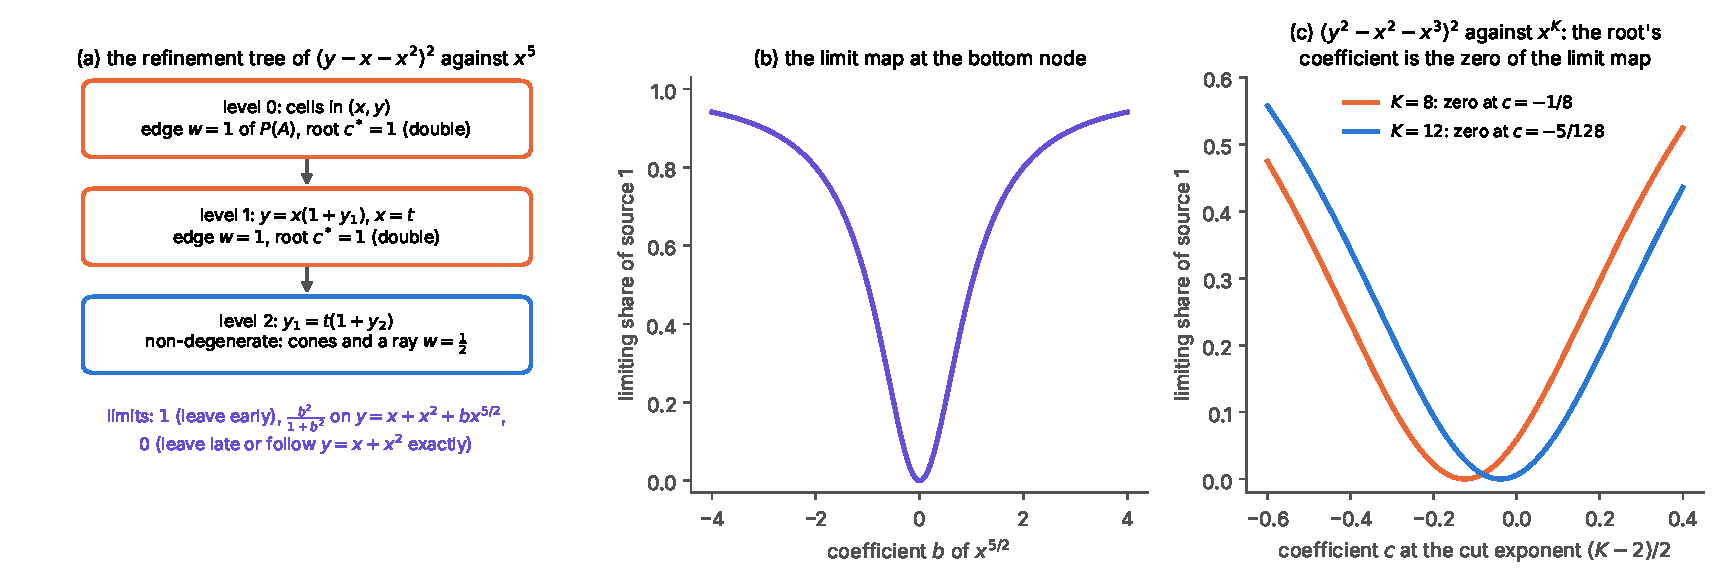
\includegraphics[width=\linewidth]{fig_degen.pdf}
\caption{Step 4f. (a) The refinement tree of \cref{ex:twolevel}. (b) The limit map at its bottom node. (c) \Cref{ex:infroot}: at the cut, the
limit map vanishes exactly at the root's coefficient ($-\tfrac18$ for $K=8$, $-\tfrac5{128}$ for $K=12$).}\label{fig:degen}
\end{figure}

\emph{Scope.} Two parameters. For $d>2$ the same criterion holds: degeneracy is a property of $P(A)$ alone, since cells cannot cancel. The
recursion then needs a resolution of $P(A)$ rather than Newton--Puiseux, for example by toric modifications along the degenerate faces. A
termination bound there is open. Step 5 reads this recursion through the log map: degenerate
directions are exactly where the log fails (\cref{thm:logtrop}(5)).

\section{Step 5: functions, duality and logs}\label{sec:duality}
Steps 1--4 built the covariant side: laws, kernels, the monad $\D$, the comonad $W$, the tangent structure $T$. Functions were present
throughout, as events $\mathbf 1_A$, utilities $u_a$ and decision gaps, but they were never named as a side of their own. Neither were
logarithms, though the order $v$ of Step 3 is one. This step names both, adds the cotangent cone at the boundary, and collects what the
layers say about what does not matter.

\subsection{States and effects}
A law $p$ is a \emph{state}; a function $u:X\to\R$ is an \emph{effect}; $\langle u,p\rangle=\sum_xu(x)p(x)$ is their pairing. A kernel $K:X\to\D Y$ pushes
states forward, $p\mapsto pK$, and pulls effects back, $u\mapsto Ku$ with $(Ku)(x)=\sum_yK(x,y)u(y)$. This is the state-and-effect picture of
categorical probability \cite{Jacobs2015}.

\begin{center}\small
\resizebox{\linewidth}{!}{\begin{tabular}{lll}\toprule
structure & variance & where\\\midrule
$\D$, $\mu$ (laws, pooling); $W$, $\lambda$ (provenance) & covariant & Step 1\\
$T^k$ (feasible directions, Weil points) & covariant & Step 2\\
a kernel acting on states / on effects & covariant / contravariant & \cref{prop:effects}(1)\\
marginalisation $M_S=\D\pi_S$ & covariant in $\pi_S$, contravariant in the window $S\subseteq T$ & \cref{prop:marg}\\
window tables over a cover; the $L^2$ presheaf of conditional expectations & contravariant (presheaves) & covers paper; main paper, \cref{prop:effects}(6)\\
the facewise presheaf $\mathcal O$ & contravariant on the face poset & \cref{def:decorated}\\
parameterised families $P\mapsto\mathrm{Hom}(P,\Delta_{L\times X})$ & contravariant in the parameters & \cref{def:para}\\
events, utilities, decision gaps & effects (contravariant) & \cref{prop:effects}\\
the order fan (weights $w$ are functionals on exponents) & dual to the Newton polyhedron & \cref{thm:logtrop}(3)\\
the cotangent cone $C_x^*$ & contravariant & \cref{prop:cotangent}\\\bottomrule
\end{tabular}}
\end{center}

\begin{proposition}[conditioning is an update by an effect]\label{prop:effects}
\begin{enumerate}
\item[(1)] $\langle u,pK\rangle=\langle Ku,p\rangle$, and pulling back is contravariant: $(KL)u=K(Lu)$. Marginalisation pulls effects back along the
  projection, and forgetting provenance pulls $u$ back to $u\circ\epsilon$.
\item[(2)] For an effect $q\ge0$ with $\langle q,p\rangle>0$, the \emph{update} is $C_q(p)=q\,p/\langle q,p\rangle$. Then $C_A=C_{\mathbf 1_A}$, updates compose by products,
  $C_r\circ C_q=C_{qr}$, and expectations update as $\langle u,C_qp\rangle=\langle qu,p\rangle/\langle q,p\rangle$.
\item[(3)] The contextual Bayes decomposition holds for every effect. Updating the labelled law by $\epsilon^*q$ gives rows $C_q(p_l)$ and Bayes weights
  $\pi^q_l=\pi_l\langle q,p_l\rangle/\langle q,P\rangle$. \Cref{thm:bayes} is the case $q=\mathbf 1_A$.
\item[(4)] The Bayesian inverse is an update: $K^\dagger(\cdot\mid y)=C_{K\mathbf 1_y}(p)$, the update by the point effect $\mathbf 1_y$ pulled back along $K$.
\item[(5)] Pairing is natural for $\mathrm{Para}_L$: for a reparametrisation $r$, $\langle u,\Lambda\circ r\rangle=\langle u,\Lambda\rangle\circ r$.
\item[(6)] \emph{The $L^2$ presheaf.} For a law $p$, the conditional expectation $E_p[\,\cdot\mid X_S]$ is the $p$-adjoint of pulling back along $\pi_S$. It is
  idempotent and satisfies the tower property $E[E[u\mid X_T]\mid X_S]=E[u\mid X_S]$ for $S\subseteq T$. So marginalisation of states and conditional
  expectation of functions are the two faces of one restriction: the main paper's $L^2$ presheaf, read in the layers.
\end{enumerate}
\end{proposition}

\begin{proof}
(1) Exchange the sums. (2) $C_r(C_qp)=rqp/\langle r,qp\rangle$ and $\langle r,qp\rangle=\langle qr,p\rangle$; the expectation formula is the same computation. (3) Row $l$ of the
updated labelled law is $\pi_lq\,p_l/\langle q,P\rangle=\pi^q_lC_q(p_l)$. (4) $p(x)K(x,y)/\sum_{x'}p(x')K(x',y)$. (5) Pairing is pointwise in the parameter.
(6) $\langle E[u\mid X_S],v\circ\pi_S\rangle_p=\langle u,v\circ\pi_S\rangle_p$ is the defining property; idempotence and the tower property follow. FD1--FD3 check
all six exactly, in rational arithmetic.
\end{proof}

Updates compose by \emph{products} of effects. Under the log map these become sums, which is why Bayes is linear in logarithms and pooling
is not.

\subsection{The log map and the tropical limit}
For a scale $s\in(0,1)$, write $\operatorname{Log}_s(a)=\log a/\log s$. The order of Step 3 is its limit: $v(f)=\lim_{s\to0}\operatorname{Log}_sf(s)$ for germs asymptotic
to powers.

\begin{theorem}[logs and the tropical limit]\label{thm:logtrop}
\begin{enumerate}
\item[(1)] \emph{The m-side tropicalises.} For positive $a_1,\dots,a_n$,
  \[
  \min_i\operatorname{Log}_sa_i-\frac{\log n}{|\log s|}\le\operatorname{Log}_s\Bigl(\sum_ia_i\Bigr)\le\min_i\operatorname{Log}_sa_i .
  \]
  So pooling, marginalisation and every other mixture become $\min$ in the limit (\cref{thm:tropical}). This is Maslov's dequantisation.
\item[(2)] \emph{The e-side is exact.} $\log C_qp=\log q+\log p-\log\langle q,p\rangle$ at every scale; posterior log-odds add the prior log-odds and the
  log-likelihood ratio. On valuations, conditioning is tropical division by the tropical pairing:
  \[
  v(C_qp)(x)=v(q(x))+v(p(x))-\min_y\bigl(v(q(y))+v(p(y))\bigr).
  \]
\item[(3)] \emph{The order fan in log coordinates.} Along $\varepsilon=c\,s^w$, $\operatorname{Log}_s\varepsilon\to w$ and $\operatorname{Log}_sf(\varepsilon(s))\to\operatorname{trop}_wf=\min_\alpha\langle w,\alpha\rangle$. The
  function $\operatorname{trop}_wP(A)$ is concave and piecewise linear. Its domains of linearity are the vertex cones of the order fan, and its breaks are the
  walls: the positive part of the tropical hypersurface of $P(A)$ \cite{MaclaganSturmfels2015}. A monomial reparametrisation acts linearly on log
  coordinates.
\item[(4)] \emph{The m/e split.} Arithmetic mixtures (pooling: the m-flat families of information geometry) have valuation $\min(v(p),v(q))$.
  Geometric mixtures $p^{1-t}q^t/Z$ (e-flat families) have valuation $(1-t)v(p)+t\,v(q)$ minus its minimum, which is linear in $t$. Products of laws
  add valuations exactly, at every scale. So, in the limit, the dually flat pair of the main paper \cite{AmariNagaoka2000} becomes a pair of
  geometries: tropical-linear on the m-side and classically linear on the e-side.
\item[(5)] \emph{Where the log fails.} The only operation without a log image is subtraction. $v(a-b)$ is not determined by $v(a)$ and $v(b)$
  when they are equal. The degenerate directions of Step 4f and the contrasts that leave $\mathcal M_k$ in Step 4e are exactly the places where
  cancellation occurs.
\end{enumerate}
\end{theorem}

\begin{proof}
(1) $\max_ia_i\le\sum a_i\le n\max_ia_i$; divide the logarithms by $\log s<0$. (2) Take logarithms; the valuation identity is \cref{thm:tropical} applied
to $\langle q,p\rangle$. (3) $\log\varepsilon_i=w_i\log s+\log c_i$. For the germs, apply (1). A minimum of linear forms is concave and piecewise linear, with one
domain per vertex. (4) Exponents of monomial germs combine linearly under geometric mixing; products add exponents. (5)
$s-(s-s^2)=s^2$. Checks: FD4 tests (1) on $500$ random sums (largest ratio to the bound $0.90$) and (2) exactly on germs. FD5 tests (3) by
evaluation at scales $10^{-20},10^{-40},10^{-80}$ in log space, and the domain count. FD6 tests (4) exactly.
\end{proof}

\subsection{The cotangent cone at the boundary}
\begin{proposition}[the cotangent cone]\label{prop:cotangent}
Let $C_x^*=\{g:\langle g,u\rangle\ge0\text{ for all }u\in C_x\}$, with covectors taken modulo constants, and let $N_x=-C_x^*$ be the normal cone.
\begin{enumerate}
\item[(1)] $g\in C_x^*$ iff $g$ is constant, say equal to $\gamma$, on the support of $x$, and $g\ge\gamma$ on its empty cells. At a relative-interior point
  $C_x^*=0$. At the boundary it is a cone with one ray for each empty cell.
\item[(2)] \emph{Contravariance.} Every smooth map $f$ of simplices sends $C_x$ into $C_{f(x)}$, so $\mathcal M_1$ contains them all. Hence
  $Df(x)^{\mathsf T}$ maps $C^*_{f(x)}$ into $C^*_x$, and $T^*$ is a contravariant functor on dual cones.
\item[(3)] \emph{Robust ties.} Let a linear decision tie at $x$, $\langle u_a-u_b,x\rangle=0$. Then act $a$ stays weakly preferred after every first-order injection
  iff $u_a-u_b\in C_x^*$.
\item[(4)] \emph{The decision fan as a sign pattern.} Along an arc, the comparison of $a$ and $b$ is the sign of the germ $\langle u_a-u_b,\Phi(\varepsilon)\rangle$.
  Its numerator $N_{ab}=\sum_c(u_a-u_b)(c)f_c$ is a \emph{signed} polynomial. On a cone of the fan, the decision walls are the positive roots of
  $N_{ab}$'s edge polynomial, and they are resolved by \cref{thm:degen} applied to $N_{ab}$. Unlike $P(A)$, $N_{ab}$ can cancel, so decision walls
  appear in directions where the conditioned state itself is not degenerate.
\end{enumerate}
\end{proposition}

\begin{proof}
(1) Pairing with the lineality directions $e_i-e_s$ forces $g$ to be constant on the support. Pairing with the rays $e_z-e_s$ gives $g_z\ge\gamma$. (2)
If $f(\Delta)\subseteq\Delta'$, then $x+tu\in\Delta$ gives $f(x+tu)\in\Delta'$, so $Df(x)u\in C_{f(x)}$. Then
$\langle Df^{\mathsf T}g',u\rangle=\langle g',Df\,u\rangle\ge0$. (3) The first-order change of the gap along $u$ is $\langle u_a-u_b,u\rangle$. (4) The denominator $P(A)$ is
positive; then apply \cref{thm:decisionfan}. Checks: FD7 pulls $6000$ dual covectors back through stochastic maps and conditioning at
boundary points, and tests (3) against $200$ sampled injections per case. FD8 locates $9$ walls at the predicted roots and checks that the
act flips across each.
\end{proof}

\subsection{What does not matter}
The lab asked which parts of the data, the parameters and the model can be ignored for a decision \cite[Section ``What does not
matter'']{Lab}. In the language of this step, an exclusion is an annihilator, and the layers give five such statements.

\begin{proposition}[exclusion principles]\label{prop:exclusion}
Let $K$ be the window map of a cover and $\rho=(u_a-u_b)_{a,b}$ the utility gaps.
\begin{enumerate}
\item[(1)] \emph{Duality.} The data directions that do not matter are $\ker K\cap\ker\rho$. Dually, the utility gaps that are functions of the window
  tables, $\operatorname{span}\rho\cap\operatorname{im}K^{\mathsf T}$, are pinned by the data and do not matter for settling. The decision-relevant dimension of
  \cite[Proposition ``the decision-relevant quotient'']{Lab} is
  \[
  \operatorname{rank}(\rho|_{\ker K})=\dim\operatorname{span}\rho-\dim(\operatorname{span}\rho\cap\operatorname{im}K^{\mathsf T}).
  \]
\item[(2)] \emph{Conditioning.} For a decision taken after observing $A$, the following do not matter (\cref{prop:tc,prop:four}):
  \begin{itemize}
  \item the data off $A$;
  \item the total mass of $A$;
  \item the provenance off $A$;
  \item the utilities off $A$.
  \end{itemize}
\item[(3)] \emph{At the wall.} Along a cone of the order fan, every coefficient off the leading face of $N$ is irrelevant to the limit. On a
  vertex cone only the vertex's coefficients matter. Along a degenerate direction, only the coefficients at the node of \cref{thm:degen}
  that resolves it matter.
\item[(4)] \emph{Feasibility.} Subtraction-free operations never matter for feasibility at any order (\cref{thm:graded}); only contrasts do.
\item[(5)] \emph{Statistics.} In the invisible cone of \cref{thm:Jfan} an adversary does not matter: its impact vanishes. On the wall side of
  \cref{thm:poissonband}, standard errors stop mattering and counts are the right measure.
\end{enumerate}
\end{proposition}

\begin{proof}
(1) $\ker K=(\operatorname{im}K^{\mathsf T})^\perp$, so restricting $\rho$ to $\ker K$ kills exactly its part in $\operatorname{im}K^{\mathsf T}$. (2) $\langle u,C_Ap\rangle$ depends on $u$ only through $u|_A$,
and on $p$ only through $p|_A$ up to scale. (3) The limit is the normalised initial forms (\cref{prop:arc}, \cref{thm:degen}). (4) and (5) restate the
cited results. FD9 checks (1) on $40$ covers, $14$ of them with gaps pinned by a window, and checks (2) and (3) exactly.
\end{proof}

\begin{figure}[!htbp]\centering
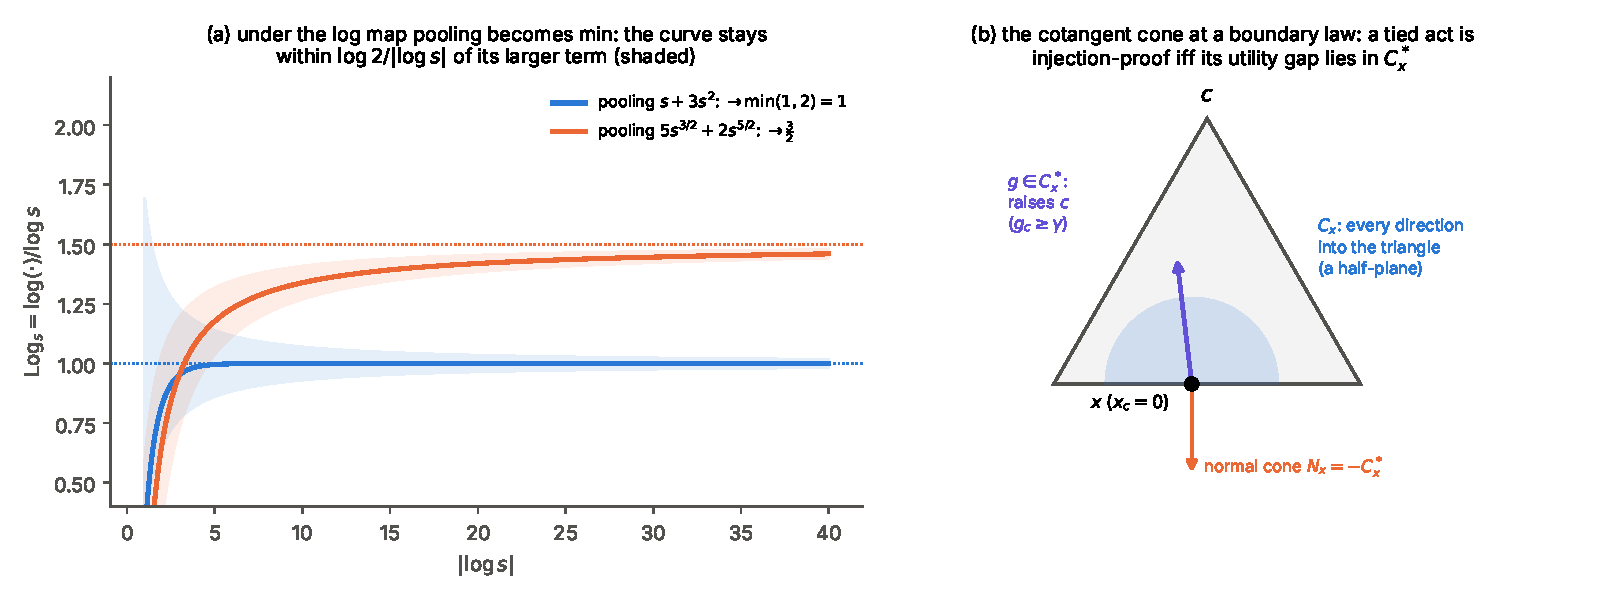
\includegraphics[width=\linewidth]{fig_duality.pdf}
\caption{Step 5. (a) Under the log map, a pooled sum stays within $\log n/|\log s|$ of its leading term and tends to the minimum of the orders
(\cref{thm:logtrop}(1)). (b) At a boundary law the feasible directions form a half-plane. Covectors in the dual cone $C_x^*$ cannot be lowered
by any injection, and a tied act is injection-proof iff its utility gap lies there (\cref{prop:cotangent}(3)).}\label{fig:duality}
\end{figure}

\section{Checks and scope}\label{sec:checks}
Step 1's checks are in \texttt{engine/check\_context.py} (module \texttt{engine/pce/context.py}; $13/13$, about a second). DL1--DL10, DL12 and
DL13 use exact rational arithmetic; DL11 uses floating point. Step 2's checks are in \texttt{engine/check\_tangent\_layers.py} (module
\texttt{engine/pce/tangent\_layers.py}; $9/9$, about $25$ seconds) and \texttt{engine/check\_jumps.py} (module \texttt{engine/pce/jumps.py}; $6/6$,
about $2$ seconds; SJ1--SJ3, SJ5 and SJ6 exact). Step 3's are in \texttt{engine/check\_orders.py} (module \texttt{engine/pce/orders.py}; $7/7$,
about $2$ seconds; OR1--OR3, OR6 and OR7 exact). Step 4a--4b's are in \texttt{engine/check\_fans.py} (module \texttt{engine/pce/fans.py};
$7/7$, about two minutes; all exact except the nested numerics of MP5 and the Weil arithmetic of MP6). Step 4c's are in
\texttt{engine/check\_para.py} (module \texttt{engine/pce/para.py}; $6/6$, under a minute; exact except the numerical comparison in PR3). Step 4d's are in \texttt{engine/check\_statfan.py} (module
\texttt{engine/pce/statfan.py}; $7/7$, about a minute; ST1--ST3 exact or Weil, ST4 floating point, ST5--ST7 Monte Carlo with fixed seeds). The Poisson band and Step 4e are in \texttt{engine/check\_graded.py} (modules
\texttt{engine/pce/poissonband.py} and \texttt{engine/pce/graded.py}; $11/11$, about two minutes). Step 4f's are in \texttt{engine/check\_degen.py}
(module \texttt{engine/pce/degen.py}; $6/6$, exact). Step 5's are in \texttt{engine/check\_effects.py} (module \texttt{engine/pce/effects.py};
$9/9$, under a minute). TL8 is exact; the others use floating point with the Weil-algebra
arithmetic of the tangent companion. The figures come from \texttt{context/fig\_layers.py}.
\begin{center}\small
\begin{tabular}{lp{0.8\textwidth}}\toprule
DL1--DL4 & the four axioms of the distributive law (\cref{prop:dist}), exactly, on $50$ random elements each\\
DL5 & the two-sided Kleisli category: explicit composite, associativity, identity\\
DL6 & marginalisation: iterated, affine, commutes with forgetting provenance\\
DL7 & conditioning: partial domain, total probability, iteration\\
DL8 & the conditioning--marginalisation square: commutes for cylinders, fails for a non-cylinder event\\
DL9 & a known source stays known; the contextual Bayes decomposition; the old weights are wrong\\
DL10 & forgetting provenance: commutes with windows, not injective, labelled windows differ\\
DL11 & $D^2M=0$; $DC_A$, $D^2C_A$ against finite differences; $\|DC_A\|\,p(A)$ constant as $p(A)\to0$\\
DL12 & no continuous extension of $C_A$ to the wall (\cref{prop:wall})\\
DL13 & the worked examples: $\tfrac8{23},\tfrac{15}{23}$; $\tfrac9{23}$ against $\tfrac{63}{160}$; $\tfrac9{19}$ against $\tfrac{23}{40}$\\\midrule
TL1 & $T$ commutes with $W$: $T^2\lambda$ lands in $T^2\Delta_{L\times X}$; counit and comultiplication on $T^2$ points (\cref{prop:tw})\\
TL2 & the source face: tangent directions stay on the row; every other feasible direction is a face direction plus an injection (\cref{prop:face})\\
TL3 & forgetting maps cones onto cones; injection and drift have the same image; relabelling is invisible\\
TL4 & marginalisation: explicit lift onto, $T^2$ into $T^2$, kernel dimension $|X|-|X_S|$, $D^2=0$ (\cref{prop:tm})\\
TL5 & conditioning: lift onto, kernel dimension $|X|-|A|$, second-order criterion and $900$ direct $T^2$ points, pole; a negative control fails both tests (\cref{prop:tc})\\
TL6 & pooling: first order into the cone, the criterion at corners including a weight-$0$ source, $1200$ direct $T^2$ points, $D^3=0$\\
TL7 & the differentiated Bayes decomposition (\cref{prop:dbayes})\\
TL8 & \cref{ex:sens} exactly: $\tfrac9{23}$, $-\tfrac{16}{529}$, $\tfrac{384}{12167}$, $\dot\pi^A_1=\tfrac{640}{529}$, and the reweighting split\\
TL9 & \cref{thm:tensor}: explicit tensor decompositions ($k\le4$), closure under products, pooling at order $3$\\\midrule
SJ1 & \cref{thm:support}, exactly, on $291$ families with zero weights and zero likelihoods\\
SJ2 & \cref{prop:four}(1)--(2), with the coinciding-conditionals example\\
SJ3 & \cref{prop:four}(3)--(4): explicit lifts, fibre dimensions, any posterior provenance, identifiability only lost\\
SJ4 & \cref{thm:regimes}(1)--(2): the rate bound on random paths, the provenance bound, an oscillating extinction\\
SJ5 & \cref{thm:regimes}(3)--(5), exactly: leading-jet limits, the smooth example, a removable passage, a kink\\
SJ6 & \cref{ex:jumps}, exactly: width $4\eta$, slope $-1/(4\eta)$, the replacement bound\\\midrule
OR1 & \cref{thm:tropical}: order is a homomorphism to $(\min,+)$ on non-negative germs; cancellation without positivity\\
OR2 & \cref{cor:calculus}: every row of the order calculus, exactly, on $200$ labelled paths\\
OR3 & \cref{thm:hierarchy}(1)--(2): limits, survivors, extinction rates, the error exponent $\delta$\\
OR4 & \cref{thm:hierarchy}(3): analytic passages agree; the $C^\infty$ flat jump\\
OR5 & \cref{thm:hierarchy}(4): Hardy (limit) against oscillating (none), in log space\\
OR6 & \cref{prop:tower}: the $k$-jet sees the transition iff $k\ge m$; the Weil coefficients $|S|!\,c_{|S|}$\\
OR7 & \cref{ex:order}, exactly: width $2(2\eta)^{1/m}$ for $m=1,2,3$\\\midrule
MP1 & \cref{prop:arc}: arc limits are normalised initial forms, exactly, $300$ families\\
MP2 & \cref{thm:fan}(1): the leading faces are the vertices and bounded edges of $N$\\
MP3 & \cref{thm:fan}(3)--(4): the componentwise-minimum criterion for monomial cells\\
MP4 & \cref{ex:race,ex:dominance,ex:curved,ex:degenerate}, exactly\\
MP5 & \cref{thm:iterated}: iterated limits are lexicographic vertices; orders disagree; corners agree while the middle differs\\
MP6 & \cref{prop:towerlex}: Weil points in $T^d$, the lemma's first term, the flip\\
MP7 & \cref{ex:curved}: lines agree, parabolas do not\\\midrule
PR1 & \cref{prop:para}(1): Para composition, identities, whiskering, exactly\\
PR2 & \cref{prop:para}(2)--(3): layer operations commute with reparametrisation; the conditioning domain pulls back\\
PR3 & the germ field: valuations are tropical orders, the standard part is the arc limit\\
PR4 & \cref{thm:decisionfan}(1)--(2): eventual acts, ties broken at higher order, against evaluation at $s=10^{-8}$\\
PR5 & \cref{ex:audit}, exactly, including the tie at $c=1$ broken at order $3$\\
PR6 & \cref{thm:decisionfan}(4) and \cref{ex:designs}: transport along monomial reparametrisations; each design fills one cone\\\midrule
ST1 & \cref{prop:decorated}(1)--(2): the presheaf restriction identities; edge limit maps join vertex limits\\
ST2 & \cref{prop:decorated}(3): one Newton polyhedron, two decorations, limit sets $[0,1]$ and $[\tfrac12,1]$\\
ST3 & \cref{prop:cross}: exact cross term; Weil coefficients; the conditioned mixed derivative\\
ST4 & \cref{thm:Jfan}(1),(3),(4): orders as slopes; the band bound; vanishing impact; no tilt\\
ST5 & \cref{thm:Jfan}(2): Monte Carlo of the three regimes\\
ST6 & \cref{prop:poisson}: Gaussian cone, Poisson ray, empirical wall (Monte Carlo)\\
ST7 & negative control: fixed $P(A)$ covers nominally\\\midrule
PB1 & \cref{thm:poissonband}(1): $k_\alpha(T+1)\le k_\alpha(T)+1$; exposure increasing; level $\le\alpha$\\
PB2 & the exact band: exposure $=\beta$ at $\mu_C^{\max}$; Monte Carlo\\
PB3 & \cref{thm:poissonband}(2): Gaussian limit to J's $B$\\
PB4 & \cref{thm:poissonband}(3): the Poisson ray and the blind spot\\
PB5 & \cref{thm:poissonband}(4): the wall side, $\lambda^*$, the adversary owns the event\\
GC1 & \cref{thm:graded}(1): the zero section; the chain\\
GC2--GC3 & \cref{thm:graded}(2): separations at orders $2$ and $3$\\
GC4 & units and inverses in $T^kH$\\
GC5 & \cref{thm:graded}(3)--(4): subtraction-free maps and the layer operations at $T^3$, $T^4$\\
GC6 & contrasts leave $\mathcal M_2$\\\midrule
DG1 & \cref{thm:degen}: recursion = direct expansion along $424$ arcs\\
DG2 & \cref{thm:degen}(1): refine iff $P(A)$'s edge polynomial vanishes; partial vanishing drops cells\\
DG3 & \cref{ex:twolevel}, exactly\\
DG4 & tree nodes are root truncations; $996$ arcs agree\\
DG5 & \cref{thm:degen}(3): multiplicities non-increasing; chains finite\\
DG6 & \cref{ex:infroot}: chain length $\tfrac{K-2}2-1$, series coefficients, the zero of the limit map\\\midrule
FD1--FD3 & \cref{prop:effects}: duality, updates by effects, Bayes weights, Bayesian inverse, Para naturality, the $L^2$ presheaf\\
FD4--FD6 & \cref{thm:logtrop}: Maslov bound, tropical division, normal fan in log coordinates, the m/e split\\
FD7--FD8 & \cref{prop:cotangent}: dual cones pulled back, robust ties, decision walls as signed roots\\
FD9 & \cref{prop:exclusion}: the annihilator identity; utilities off $A$; coefficients off the leading face\\\bottomrule
\end{tabular}
\end{center}
\emph{Scope.} Finite sets and discrete, known sources. Step 2 settles first order for every operation, order two for conditioning (every order, by Step 4e), and
every order for forgetting, marginalisation, the source embedding and pooling. It classifies where conditioned probabilities can
jump on finite sets. Step 3 gives the order calculus of transitions along one-parameter paths, and Step 4a--4b extends it to several
parameters for polynomial cells (a full existence criterion for general polynomial cells is open). Step 4c attaches decisions to the fan, and Step 4d derives Theorem J's band from the cross term under J's Gaussian model
(\cref{thm:Jfan}). Step 4d adds an exact band on the Poisson ray, and Step 4e shows that every layer
operation, conditioning included, keeps feasibility at every order. Step 4f resolves degenerate directions recursively for two parameters. Open: termination
bounds for more than two parameters, and bands for decoration-dependent decisions near walls.

\begin{thebibliography}{99}
\bibitem{Lab} V.~K.~Awasthi, A lab for latent actors: hiding segments, probes, settled decisions, injected records and sources, 2026.
\bibitem{CoversCompanion} V.~K.~Awasthi, Two latent types on arbitrary covers, Part I: pair graphs, sign sheets and hiding polytopes, companion paper, 2026.
\bibitem{TangentCompanion} V.~K.~Awasthi, A tangent structure for injected data: feasible cones, universality at corners, jets on the tetrad scheme, companion paper, 2026.
\bibitem{AbramskyBrandenburger2011} S.~Abramsky and A.~Brandenburger, The sheaf-theoretic structure of non-locality and contextuality, \emph{New J. Phys.} \textbf{13} (2011) 113036.
\bibitem{Giry1982} M.~Giry, A categorical approach to probability theory, in \emph{Categorical Aspects of Topology and Analysis}, Lecture Notes in Math. \textbf{915}, Springer, 1982, 68--85.
\bibitem{Fritz2020} T.~Fritz, A synthetic approach to Markov kernels, conditional independence and theorems on sufficient statistics, \emph{Adv. Math.} \textbf{370} (2020) 107239.
\bibitem{FritzPerrone2018} T.~Fritz and P.~Perrone, Bimonoidal structure of probability monads, \emph{Electron. Notes Theor. Comput. Sci.} \textbf{341} (2018) 121--149.
\bibitem{Jacobs2018} B.~Jacobs, From probability monads to commutative effectuses, \emph{J. Log. Algebr. Methods Program.} \textbf{94} (2018) 200--237.
\bibitem{ChoJacobs2019} K.~Cho and B.~Jacobs, Disintegration and Bayesian inversion via string diagrams, \emph{Math. Struct. Comput. Sci.} \textbf{29} (2019) 938--971.
\bibitem{Simpson2017} A.~Simpson, Probability sheaves and the Giry monad, in \emph{CALCO 2017}, LIPIcs \textbf{72} (2017) 1:1--1:6.
\bibitem{UustaluVene2008} T.~Uustalu and V.~Vene, Comonadic notions of computation, \emph{Electron. Notes Theor. Comput. Sci.} \textbf{203} (2008) 263--284.
\bibitem{PowerWatanabe2002} J.~Power and H.~Watanabe, Combining a monad and a comonad, \emph{Theoret. Comput. Sci.} \textbf{280} (2002) 137--162.
\bibitem{Hardy1910} G.~H.~Hardy, \emph{Orders of Infinity: The `Infinit\"arcalc\"ul' of Paul du Bois-Reymond}, Cambridge Tracts in Mathematics \textbf{12}, Cambridge University Press, 1910.
\bibitem{Rosenlicht1983} M.~Rosenlicht, Hardy fields, \emph{J. Math. Anal. Appl.} \textbf{93} (1983) 297--311.
\bibitem{FongSpivakTuyeras2019} B.~Fong, D.~Spivak and R.~Tuy\'eras, Backprop as functor: a compositional perspective on supervised learning, in \emph{Proc. LICS 2019}, IEEE, 2019.
\bibitem{CruttwellEtAl2022} G.~S.~H.~Cruttwell, B.~Gavranovi\'c, N.~Ghani, P.~Wilson and F.~Zanasi, Categorical foundations of gradient-based learning, in \emph{ESOP 2022}, Lecture Notes in Comput. Sci. \textbf{13240}, Springer, 2022, 1--28.
\bibitem{Curry2014} J.~Curry, \emph{Sheaves, Cosheaves and Applications}, PhD thesis, University of Pennsylvania, 2014.
\bibitem{Walker1950} R.~J.~Walker, \emph{Algebraic Curves}, Princeton University Press, 1950.
\bibitem{CasasAlvero2000} E.~Casas-Alvero, \emph{Singularities of Plane Curves}, London Math. Soc. Lecture Note Ser. \textbf{276}, Cambridge University Press, 2000.
\bibitem{Jacobs2015} B.~Jacobs, New directions in categorical logic, for classical, probabilistic and quantum logic, \emph{Log. Methods Comput. Sci.} \textbf{11}(3) (2015) 24.
\bibitem{MaclaganSturmfels2015} D.~Maclagan and B.~Sturmfels, \emph{Introduction to Tropical Geometry}, Graduate Studies in Mathematics \textbf{161}, AMS, 2015.
\bibitem{AmariNagaoka2000} S.~Amari and H.~Nagaoka, \emph{Methods of Information Geometry}, AMS and Oxford University Press, 2000.
\bibitem{Milnor1968} J.~Milnor, \emph{Singular Points of Complex Hypersurfaces}, Annals of Mathematics Studies \textbf{61}, Princeton University Press, 1968.
\bibitem{BrookesVanStone1993} S.~Brookes and K.~Van Stone, Monads and comonads in intensional semantics, Technical Report CMU-CS-93-140, Carnegie Mellon University, 1993.
\end{thebibliography}

\appendix
\input{../shared/symbols}
\input{../shared/status}
\end{document}
